%%%%%%%%%%%%
%% Please rename this main.tex file and the output PDF to
%% [lastname_firstname_graduationyear]
%% before submission.
%%%%%%%%%%%%

\documentclass[12pt]{caltech_thesis}
\usepackage[hyphens]{url}
\usepackage{lipsum}
\usepackage{graphicx}
\usepackage{xcolor}
\usepackage{longtable}
\usepackage{pdflscape}
\usepackage{deluxetable}

%\usepackage{todonotes}

%% Tentative: newtx for better-looking Times
\usepackage[utf8]{inputenc}
\usepackage[T1]{fontenc}
\usepackage{newtxtext,newtxmath}


% Must use biblatex to produce the Published Contents and Contributions, per-chapter bibliography (if desired), etc.
\usepackage[
    backend=biber,natbib,
    %backend=natbib,
    % IMPORTANT: load a style suitable for your discipline
    style=authoryear-comp,
    uniquelist=false,
    doi=False,
    %maxalphanames=1,
    %labelalpha,
    %sorting=ynt,
    bibstyle=apj, 
]{biblatex}
\renewcommand*{\nameyeardelim}{\addspace}
%\usepackage{natbib}
%\bibliographystyle{apj}
\newcommand{\todo}[3]{{\color{#2} \emph{#1} TO DO: #3}}
\newcommand{\btmtodo}[1]{\todo{BEN}{red}{#1}}

\renewcommand{\d}[1]{\ensuremath{\operatorname{d}\!{#1}}}
\newcommand{\rsun}{{R$_\odot$}}
\newcommand{\msun}{{M$_\odot$}}
\newcommand{\kep}{{\textit Kepler}}
\newcommand{\KT}{{\textit K2}}
\newcommand{\eg}{{\it e.g.}}
\newcommand{\ie}{{\it i.e.}}
\newcommand{\spitz}{{\textit Spitzer}}
\newcommand{\vsini}{{$V \sin i$}}
\newcommand{\teff}{$T_{\rm eff}$}
\newcommand{\kms}{{km\,s$^{-1}$}}
\newcommand{\gcc}{{g\,cm$^{-3}$}}
\newcommand{\rstar}{{$R_\star$}}
\newcommand{\mstar}{{$M_\star$}}
\newcommand{\rhostar}{{$\rho_\star$}}
\newcommand{\mearth}{{M$_\oplus$}}
\newcommand{\rearth}{{R$_\oplus$}}
\newcommand{\mjup}{{M$_\textrm{Jup}$}}
\newcommand{\rjup}{{R$_\textrm{Jup}$}}

\newcommand{\procspie}{SPIE Proceedings}
\newcommand{\aj}{AJ}
\newcommand{\pasp}{PASP}
\newcommand{\apj}{ApJ}
\newcommand{\apjl}{ApJL}
\newcommand{\apjs}{ApJS}
\newcommand{\aap}{A\&A}
\newcommand{\mnras}{MNRAS}
\newcommand{\sci}{Science}
\newcommand{\nat}{Nature}
\newcommand{\aapr}{Astronomy and Astrophysics Review}
\newcommand{\actaa}{Acta Astronomica}
\newcommand{\araa}{Annual Review of Astron. and Astrophys.}
\newcommand{\aaps}{Astronomy and Astrophysics, Supplement}

% Name of your .bib file(s)
\addbibresource{exopapers.bib}


\begin{document}

% Do remember to remove the square bracket!
\title{Low-Mass Stars and Their Companions}
\author{Benjamin Tyler Montet}

\degreeaward{Doctor of Philosophy}                 % Degree to be awarded
\university{California Institute of Technology}    % Institution name
\address{Pasadena, California}                     % Institution address
\unilogo{caltech.png}                                 % Institution logo
\copyyear{2017}  % Year (of graduation) on diploma
\defenddate{July 18, 2016}          % Date of defense

\orcid{0000-0001-7516-8308}

\rightsstatement{All rights reserved except where otherwise noted}


\maketitle[logo]


\begin{acknowledgements} 	 
I am extremely grateful to everyone who has helped me get to Caltech, as well as those
who have helped me through these past five years.
Of course, this list must begin with my parents: thank you for all your support and
encouragement over the past 27 years.
I also want to thank my fifth grade teacher, Mrs.\ Kim Klappauf, for always being so
enthusiastic and showing us that being into science was cool.

I want to thank my advisor, John Johnson, and everyone involved in the Exolab during 
my time. 
That (long!) list includes Justin Crepp, Phil Muirhead, Leslie Rogers,
Brendan Bowler, Jennifer Yee, and Luan Ghezzi for allowing them to regularly bug them with
questions in their offices.
I especially want to thank Jon Swift for his patience in working through problems on the
white board, his pedantry in third order corrections, and his enthusiasm for life both
inside and out of Cahill.

I want to thank everyone involved with the Summer 2013 ``Modern Statistical and
Computational Methods for Analysis of Kepler Data'' workshop at the Statistical and
Applied Mathematical Sciences Institute in Research Triangle Park, North Carolina.
The workshop certainly changed the trajectory of my thesis, and allowed me to meet 
new friends and collaborators. 
I thank the organizers, especially Eric Ford and David Hogg (the latter whom, I
acknowledge formally,
I still owe a bottle of good wine), for allowing me to participate, and the participants
for being so amazing, especially Ruth, Dan, Robert, Megan, Ben, Angie, and Gal.

I want to thank the Caltech Astronomy graduate students for being the friendliest, 
most pleasant classmates and friends one could ask for. 
I particularly want to thank (in no particular order) Mislav, Antonija, Trevor, Allison, Yi, Matt, Sirio,
Gwen, Drew, Ryan and Donal. 
To my officemates Walter, Shriharsh, Drew, Sirio, and Mislav: thank you for putting up
with me. Sorry I took away your couch (if it's any consolation, it looks nice in my 
apartment.)
I also want to thank the faculty for allowing the graduate community to be what it is, 
especially Wal Sargent. I still miss seeing your face around the department and hearing
your opinions on everything from iced tea to camping. And football, especially football.

I will always remember the traditions shared among the Cahill grad students: 
ski trips to Mammoth (never Big Bear, sorry Trevor), Wednesday night softball with the Big Bangers,
Halloween parties, trips to the Athenaeum, wine and cheese, concerts at the Hollywood
Bowl, finding space for 15 people to eat lunch together at Chandler, and so much more.

I would like to thank my committee: Heather Knutson, Gregg Hallinan, Phil Hopkins, and
Tony Readhead for reading my thesis (at least this far) and for their support and
guidance.
I also want to thank Patrick Shopbell, Anu Mahabal, and Jos\'e Calderon, who must form
the best computing staff in all of astronomy.

Finally, I want to thank Laura. Thank you for your support. 
Thank you for always being there when I need someone.
Thank you for always being there when I need someone to put me in my place.
I've enjoyed every day of our adventure, and I can't wait to see what happens next.
   
   
\end{acknowledgements}

\begin{abstract}
In this thesis, I present seven studies aimed towards better understanding the demographics
and physical properties of M dwarfs and their companions.
These studies focus in turn on planetary, brown dwarf, and stellar companions to M dwarfs.

I begin with an analysis of radial velocity and transit timing analyses of multi-transiting
planetary systems, finding that if both signals are measured to sufficiently high precision
the stellar and planetary masses can be measured to a high precision, eliminating a need
for stellar models which may have systematic errors.
I then combine long-term radial velocity monitoring and a direct imaging
campaign to measure the occurrence rate of giant planets around M dwarfs.
I find that $6.5\% \pm 3.0\%$ of M dwarfs host a Jupiter mass or larger planet within
20 AU, with a strong dependence on stellar metallicity.

I then present two papers analyzing the LHS\,6343 system, which contains a widely
separated M dwarf binary (AB).
Star A hosts a transiting brown dwarf (LHS\,6343\,C) with a 12.7 day period.
By combining radial velocity data with transit photometry, I am able to measure
the mass and radius of the brown dwarf to 2\% precision, the most precise measurement
of a brown dwarf to date.
I then analyze four secondary eclipses of the LHS\,6343\,AC system as observed by \spitz\
in order to measure the luminosity of the brown dwarf in both \spitz\ bandpasses.
I find the brown dwarf is consistent with theoretical models of an 1100 K T dwarf at an
age of 5 Gyr and empirical observations of field T5-6 dwarfs with temperatures of 
$1070 \pm 130$ K.
This is the first non-inflated brown dwarf with a measured mass, radius, and multi-band
photometry, making it an ideal test of evolutionary models of field brown dwarfs.

Next, I present the results of an astrometric and radial velocity campaign to measure the
orbit and masses of both stars in the GJ\,3305\,AB system, an M+M binary comoving with
51\,Eridani, a more massive star with a directly imaged planetary companion.
I compare the masses of both stars to largely untested theoretical models of young M 
dwarfs, finding that the models are consistent with the measured mass of star A but 
slightly overpredict the luminosity of star B.

In the final two science chapters I focus on space-based transit surveys, present and
future.
First, I present the first catalog of statistically validated planets from the \KT\ mission, as well as updated stellar and planetary parameters for all systems with candidate
planets in the first \KT\ field.
The catalog includes K2-18b, a ``mini-Neptune'' planet that receives a stellar insolation
consistent with the level that the Earth receives from the Sun, making it a useful
comparison against planets of a similar size that are highly irradiated, such as GJ\,1214\,b.
Finally, I present predictions for the \textit{WFIRST} mission. 
While designed largely as a microlensing mission, I find it will be able to detect
as many as 30,000 transiting planets towards the galactic bulge, providing
information about how planet occurrence changes across the galaxy.
These planets will be able to be confirmed largely through direct detection of their
secondary eclipses.
Moreover, I find that more than 50\% of the planets it detects smaller than Neptune 
will be found around M dwarf hosts.



\end{abstract}

%% Uncomment the `iknowhattodo' option to dismiss the instruction in the PDF.
%\begin{publishedcontent}%[iknowwhattodo]
% List your publications and contributions here.
%\nocite{Cahn:etal:2015}
%\end{publishedcontent}

\tableofcontents
\listoffigures
\listoftables
%\printnomenclature

\mainmatter

\chapter{Introduction}

\section{The M Dwarf Spectral Class}
For thousands of years, humans have studied stellar astronomy. 
The ancient Greeks, especially Hipparchos, measured the brightness and position of hundreds 
of stars.
The ancient Egyptians used observations of stars, particularly Sirius and Thuban, to measure
time for agricultural purposes.
The ancient Chinese observed supernovae for divination purposes.
Stars are one of the primary ways we can observe the universe. 
On large scales, the galaxies we observe at high redshifts are made up of stars;
on small scales, the asteroids we observe in our solar system are observable because they are
reflecting light from our
own sun.
In these cases, we can only understand the astrophysical phenomena we observe because we 
understand the starlight that creates these phenomena.

Different stars are divided into different spectral classes based on their observable spectroscopic
features.
Type M dwarfs were a part of the original Draper Catalogue of Stellar Spectra \citep{Pickering90}, 
classified as having weak but non-zero hydrogen absorption features in their spectra.
The system was alphabetical: they were classified between K and O stars, 
the former having stronger hydrogen absorption and the latter none at all.
With the development of the Harvard system, \citet{Cannon01} preserved the M spectral class and placed it
at one end of the classification system, next to K stars.
We now know that M and O stars have little hydrogen absorption in their atmospheres for very different reasons
and the modern classification system maps stellar effective temperature: M dwarfs are the coolest main-sequence
stars and the least massive hydrogen burning stars in the galaxy.
Today, the boundary between K and M dwarfs is defined by the presence of titanium oxide (TiO) bands in the
atmospheres of M dwarfs \citep{Kuiper38, Morgan38}, which can form when a star's effective temperature is below approximately 3500 K.

The single classification for M dwarfs can give the appearance of M dwarfs as a single, monolithic block.
Indeed, this is largely true for other spectral types.
The Sun has a radiative core, in which nuclear reactions are dominated by the p-p chain, and a convective 
outer layer, which contributes to the existence of a magnetic field.
The same is true for stars from the middle of the F spectral class through early M dwarfs.
M dwarfs, meanwhile, have an incredible diversity.
The M dwarf class spans an order of magnitude in mass, 
an order of magnitude in radius, and
a factor of 40 in luminosity \citep{Veeder74}.
There are significant changes in the structure of the stars across this class as well.
Below approximately 0.35 \msun, M dwarfs become fully convective, leading to a
rapid decrease in the radius and luminosity of stars just below this boundary \citep{Chabrier97}.
At the late edge of the M dwarf class are brown dwarfs, objects without high enough central densities to 
fuse hydrogen. 

In terms of their structure, F7 and K3 
dwarfs have more in common than M0 and M9 dwarfs.
Some of the stars even vary in time.
As a brown dwarf leaves the T Tauri stage of stellar evolution it has a temperature of approximately 3000 K
and a spectrum consistent with that of a mid-M dwarf.
Brown dwarfs then cool and evolve into ``late-type'' L, T, and eventually Y dwarfs at a rate 
which depends on their mass.
I will discuss the evolution of brown dwarfs more fully in Section \ref{sec:BDs}.
If the abundance of M dwarfs and the diversity of their structure had been understood at the time of the development 
of the Harvard stellar classification system, it is possible that these stars would have been awarded more than a 
single spectral type.






\section{M Dwarfs: The Silent Majority}
The early work on stellar spectroscopic classification of type M stars is based on
spectroscopy of M giants. 
The
Draper catalogue was first published in 1890 and the
Harvard stellar classification scheme in 1901,
but 
the first spectrum of an M dwarf was obtained only 100 years ago when 
\citet{Adams13} collected an observation of the M+M binary Groombridge 34.
This 8th magnitude star was known to be peculiar relative to the M stars with known spectra because of its 
high proper motion of 3 arcseconds per year; today we know it is within 4 parsec of the Sun.

The oldest known surviving diagram plotting stellar absolute magnitude against spectral type \citep{Russell14}, now known as a Hertsprung-Russell Diagram, includes hundreds of stars, as shown in Figure \ref{fig:HR}.
Today we know that M dwarfs make up approximately 75\% of the stars in the galaxy,
yet only $\sim$5\% of the stars included in Russell's figure are listed as
spectral type M. These stars are absent in the original work because they are
intrinsically faint.



\begin{figure}[hbt!]
\centering
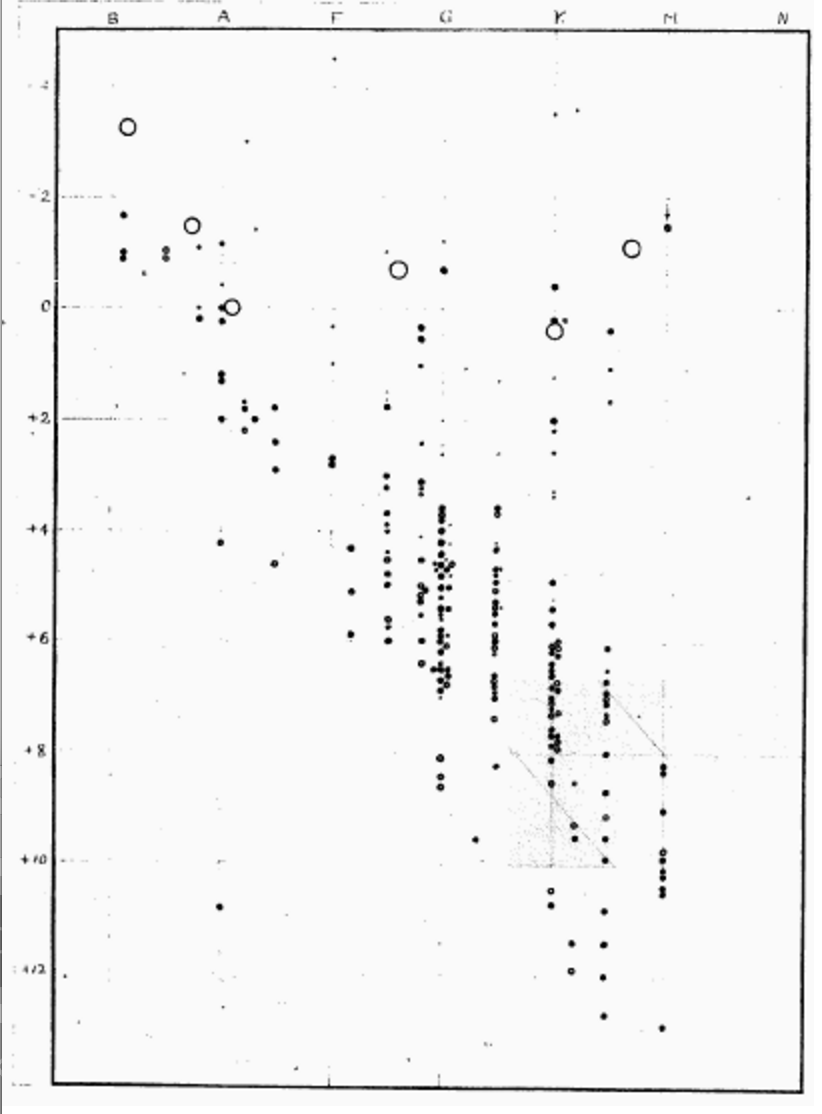
\includegraphics[width=.5\textwidth]{chapter1/hr.png}
\caption[Russell's original H-R Diagram]{The original H-R diagram, as published by
\citet{Russell14}. On the $y$-axis is absolute magnitude, equivalent to the logarithm
of the star's luminosity. On the $x$-axis is stellar spectral type, which we now know
maps approximately to stellar effective temperature.}
\label{fig:HR}
\end{figure}

The faintness of M dwarfs is the result of the physics of their interior, 
specifically the stellar mass-luminosity relation.
To show this, let us begin with the equations of stellar structure.
The first of these declares a star is in hydrostatic equilibrium:
\begin{equation}
\frac{\d P(r)}{\d r} = - \frac{ G m \rho}{r^2 },
\label{eq:hydro}
\end{equation}
where $P(r)$ is the pressure exerted on a particle at a radius $r$, $G$ is Newton's
constant, $m$ the mass enclosed inside the radius $r$, and $\rho$ the stellar density,
itself a function of radius as well.

The second equation defines mass conservation:
\begin{equation}
\frac{\d m(r)}{\d r} = 4 \pi r^2 \rho,
\end{equation}
where $\pi$ is the ratio of a circle's circumference to its diameter,
and all other variables retain their meaning from Equation \ref{eq:hydro}.

The third equation defines energy transport:
\begin{equation}
\frac{\d L(r)}{\d r} = 4 \pi r^2 \rho \epsilon,
\end{equation}
where $L$ is the energy leaving a spherical shell of radius $r$, produced by the
material in the star interior to $r$ and $\epsilon$ is the energy released per unit
mass per second inside the star.

The final equation defines the temperature gradient inside a star. 
The exact form of this equation depends on the method for which energy is transported
inside the star.
For radiative transport, the temperature gradient is
\begin{equation}
\frac{\d T}{\d r} = - \frac{3}{4ac} \frac{\bar{\kappa} \rho}{T^3} \frac{L}{4\pi r^2}.
\end{equation}
Here, $T$ is the temperature of the star at a radius $r$, $ac$ is the radiation constant multiplied by the speed of light, also equal to four times the Stefan-Boltzmann
constant, and $\bar{\kappa}$ the mean opacity of the material.

Very low-mass stars are fully convective, not radiative, and therefore follow
a different limit:
\begin{equation}
\frac{\d T}{\d r} =  \bigg( 1 - \frac{1}{\gamma}\bigg)\frac{T}{P}\frac{\d P(r)}{\d r},
\end{equation}
where $\gamma$ is the adiabatic index, and is $5/3$ for a monatomic ideal gas,
and all other terms retain their previous meaning.

Let us consider two other proportionalities. First, we assume that the energy generation rate
inside a star is a function of its temperature and density:
\begin{equation}
\epsilon = \epsilon_0 \rho T^\nu
\end{equation}
where $\nu$ depends on the particular fusion pathway that is dominant in the core of
the star.
Second, we assume that the ideal gas law holds:
\begin{equation}
P \propto \rho T.
\end{equation}

With these six equations, we can develop a series of homology relations. We can create
a series of five linear equations with five unknown parameters: $\log T$, $\log P$, 
$\log R$, $\log \rho$, and $\log M$.
Ignoring constant terms and considering only the adiabatic case (as for fully 
convective stars),
\begin{align}
\log P &= 2 \log M - 4 \log R \nonumber \\
\log \rho &= \log M - 3 \log R \nonumber \\
\log P &= \gamma \log \rho \\
\log T &= \bigg(\frac{\gamma - 1}{\gamma}\bigg) \log P \nonumber \\
\log L &= \log \rho + \nu \log T + \log M \nonumber.
\end{align}
We can rearrange these to solve for $\log M$, finding
\begin{equation}
\log R = \bigg(\frac{2-\gamma}{4 - 3\gamma}\bigg) \log M,
\end{equation}
which we can then insert into the final equation in Equation 1.8.
This manipulation yields
\begin{equation}
\log L = \bigg(\frac{2(\nu + 1) - \gamma(2\nu + 3)}{4 - 3\gamma}\bigg) \log M,
\end{equation}
which if we consider the case where we have an ideal, fully ionized gas so that $\gamma = 5/3$ and energy generation dominated by the p-p chain so that $\nu = 4$, we find
\begin{equation}
\log L \approx 8.33 \log M + \textrm{const},
\end{equation}
or $L \propto M^{8.33}$! Thus, if we decrease the mass of a fully convective star by a factor of two, 
we also decrease its luminosity by a factor of 320!\footnote{The same manipulation,
considering the case of radiative transport, leads to the relation $L~\propto~M^{5.5}$,
similar to what is observed for Sunlike stars.} 

We can take a similar approach to understand the relation between the mass and temperature of low-mass stars.
We know that
\begin{equation}
L = 4 \pi R^2 \sigma T^4,
\end{equation}
so that
\begin{equation}
\log L = 2 \log R + 4 \log T + \textrm{const.}
\end{equation}
With equations 1.9 and 1.10, we can find a relation between the log of the star's mass and its temperature:
\begin{equation}
4 \log T =  \bigg(\frac{2(\nu + 1) - \gamma(2\nu + 3)}{4 - 3\gamma}\bigg) \log M - 2 \bigg(\frac{2-\gamma}{4 - 3\gamma}\bigg) \log M + \textrm{const.}
\end{equation}
Again we consider the case where we have an ideal, ionized gas and energy generation dominated by the p-p chain, so that
$\gamma = 5/3$ and $\nu = 4$.
In this case, $\log T \approx 0.44 \log M$, so $T \propto M^{0.44}$. 
M dwarfs, with effective temperatures around 3,000 Kelvin, have significant molecular absorption in their atmospheres,
complicating their analysis even further.


Even worse for optical observing,
the peak of the SED of a typical 3,000 K M dwarf peaks at 1 micron, well into the infrared, making them even fainter in the optical.
Even though M dwarfs make up 70\% of the nearest stars, with 250 of them located within
10 pc of the Sun \citep[e.g.][]{Henry06}, there are no M dwarfs visible to the naked 
eye.
The brightest, HIP\,105090, is only $3.95 \pm 0.01$ pc from the Sun, yet has an apparent V-band magnitude of 6.76 \citep{vanLeeuwen07}.
With so many bright solar-type stars in the solar neighborhood, it is easy to understand why M dwarfs have been and often continue to be overlooked in planet search
surveys. 

\section{Radial Velocity Planet Searches}
\subsection{Stellar Radial Velocities}
Planets do not orbit their host stars.
Planets and stars, like any pair of bodies orbiting each other, orbit their common
center of mass, or barycenter.
For circular orbits, the planet and star velocities are constant, and the observed
radial component of the velocity is modulated sinusoidally with the period of the planet
as the velocity vector changes direction.
The magnitude of the RV signal in this case depends only the mass of the planet, $m$, 
the mass of the star, $M$, the orbital period, $P$, and the unknown inclination $i$.
Specifically, by taking the time derivative of the position of the star in time,
the RV can be shown to be
\begin{equation}
v_r = \bigg(\frac{2\pi G}{P}\bigg)^{1/3} \frac{m \sin i}{(M+m)^{2/3}} \cos{\nu}.
\end{equation}
Here, $G$ is Newton's constant and $\nu$ the mean anomaly of the planet, which in the circular case increases
linearly from $0$ to $2\pi$ in time over the course of one orbit.
For Jupiter, the Sun's reflex RV motion is 13 m s$^{-1}$; for Earth, 9 cm s$^{-1}$.
We see that the velocity depends on the mass ratio between the planet and star, meaning
that we can only characterize the planet as well as we understand the star.

For planets on eccentric orbits, the math is more complicated.
Again, the derivation begins with the time derivative of the position of the star, but
in the eccentric case neither the linear or angular velocity is constant \citep{Kepler09}.
It can be shown that the radial velocity equation becomes
\begin{equation}
v_r = \bigg(\frac{2\pi G}{P}\bigg)^{1/3} \frac{m \sin i}{(M+m)^{2/3}} \frac{1}{\sqrt{1-e^2}}
(e \cos \omega + \cos(\omega + \nu)),
\label{eq:rv}
\end{equation}
where $e$ is the eccentricity and $\omega$ the argument of periapsis, the angle relative
to the plane of the sky at which the planet and star make their closest approach.
All other terms retain their previous meaning, but from Kepler's second law, the true anomaly 
no longer increases linearly in time.
While we can easily measure the expected RV of the star at any position in its 
orbit, we do not know the time at which the star will be at that position.

To calculate the expected RV at a given time, we invoke the mean anomaly, which represents the mean angular motion of the 
two bodies. 
It is defined to be zero at the time of periapsis, $\tau$, and at all other times $t$ can 
be calculated such that
\begin{equation}
M = \frac{2\pi}{P}(t-\tau).
\end{equation}
It therefore increases linearly in time from 0 to $2\pi$.
The true anomaly can be calculated from the mean anomaly through the eccentric anomaly, 
$E$, such that
\begin{equation}
M = E - e \sin E.
\end{equation}
This is a transcendental equation and requires an approximate numerical solution.
Once the eccentric anomaly is determined, the true anomaly can be determined as well,
such that
\begin{equation}
\tan \frac{\nu}{2} = \sqrt{\frac{1+e}{1-e}} \tan \frac{E}{2}.
\end{equation}
With that, we can solve Equation \ref{eq:rv} and measure the RV of a star at any time.
We note that all three anomalies are identical in the circular case.

Of course, we can only use these equations if we can measure variations in the stellar RV
itself.
Fortunately, we can leverage stellar atmospheres for this purpose.
Stars with masses below $\approx 1.3$ \msun\ have convective outer layers, generating
magnetic activity which provides a torque as charged particles escape their 
host star along magnetic
field lines \citep{Shu94}.
The spin-down is a predictable function of the star's mass and age, leading to the use
of rotation rates as a probe of stellar ages \citep{Barnes03}.
G dwarfs at the age of the Sun rotate at only 1 km s$^{-1}$ at their equators.
With a full spectrum of spectral lines to consider, the RV of the star can be 
measured to 2-5 m s$^{-1}$ depending on the instrument.
At this level, systematic effects induced by the instrument can dominate over any planetary
signal: in the typical mode used for planet searches,
the resolution of Keck/HIRES is 55,000, leading to a pixel scale of 5.5 km s$^{-1}$ pixel$^{-1}$.

To measure precise RVs, both the pixel scale and a precise wavelength calibration must be
known, at a level much smaller than a single pixel.
During a night, the shape of the instrumental profile of the detector can change, leading to 
changes in the wavelength calibration considerably larger than the planetary signals
targeted.
To combat this, one of two approaches are taken.
At Keck/HIRES, observers place an iodine cell in the light path before the starlight
enters the instrument itself \citep{Butler96}.
Iodine has many absorption features in the optical with precisely known wavelengths,
so the cell creates a precise, stable wavelength scale to compare against the stellar
signal. 
The iodine also provides information about the shape of the instrumental profile during
each observation.
At other telescopes, including HARPS, the spectrograph slit is replaced with a fiber,
and the instrument is placed in a temperature and pressure controlled enclosure to keep
the instrumental profile consistent. 
Simultaneously with the observations of the stellar spectrum, a Thorium-Argon lamp is observed
which serves the same purposes as the iodine cell, providing a simultaneous wavelength
reference.


\subsection{History of RV Searches}
The first radial velocity (RV) planet searches focused almost exclusively on Sunlike
(FGK) stars, a reasonable choice as these are the brightest main sequence stars for 
which magnetic braking occurs, leading to slow rotation \citep{Wright04}.

The first planet detected around a main sequence star other than the Sun was discovered
in 1995 with the detection of 51\,Pegasi\,b, a planet with an orbital period of 4.23 days
and a mass of $0.472 \pm 0.039$ \mjup\ \citep{Mayor95}.
Quickly, dozens of similar ``hot Jupiter'' planets with masses larger than Saturn but 
periods around three days were discovered \citep[e.g.][]{Butler97, Marcy98, Wright07}.

As more planets were detected around FGK dwarfs, surveys expanded to include other
types of stars.
As stated previously, A stars do not make ideal RV survey targets due to their rapid
rotation.
However, when these stars evolve off the main sequence onto the subgiant branch,
conservation of angular momentum results in a large increase in the rotation period and
thus a decrease in $v \sin i$, making these stars amenable to RV planet searches.
These ``Retired A stars'' were found to have fewer hot Jupiters than their less massive
counterparts, but a higher giant planet occurrence rate overall \citep{Johnson07b,
Bowler10, Johnson11b}.

M dwarfs have many narrow spectral features and make ideal planet search targets as
long as they are near enough to be observable.
Indeed, the 13th planet discovered via RVs was a 2.3 \mjup\ planet in a 61-day orbit around GJ\,876  
\citep{Delfosse98, Marcy98}.
Researches detected more giant planets around M dwarfs \citep{Butler04, Butler06}, but the occurrence rate of giant planets around M dwarfs was found to be 
considerably lower than around higher mass stars.
Only $\approx 3\%$ of M dwarfs host a planet at least as massive as Jupiter 
within 2.5 AU \citep{Johnson10a, Bonfils13}.
These surveys also showed a correlation between giant planet occurrence and stellar
metallicity \citep{Fischer05, JohnsonApps09}.



To date nearly 600 planets have been discovered via RV variations.
These results show hot Jupiters orbit approximately 1\% of Sunlike stars \citep{Wright12}.
They also show that 10\% of systems have a Saturn-mass or larger planet with orbital periods
shorter than 2000 days \citep{Cumming08}.
By extrapolating the observed distribution outward, the same authors predict 20\% of FGK dwarfs host a gas giant planet within 20 AU.

Despite the large numbers of planets detected so far, RV surveys have substantial
limitations.
There has been substantial work on improving RV precision, both
in instrument development and in understanding stellar activity \citep{Fischer16}.
Yet there is still work to do: even the smallest RV signal claimed as a planetary
detection has a Doppler amplitude larger than the Earth's by a factor of six
\citep{Dumusque12}. 
Worse yet, the planet's very existence has been called into question:
the purported signal may be
an artifact of the stellar activity modeling techniques applied to the data
\citep{Rajpaul16}.

RV surveys are generally only sensitive to planets which have completed
one full orbit.
For longer periods, there is a degeneracy between the companion mass and orbital period
that cannot be broken without substantial curvature in the orbit, meaning planetary
parameters cannot be uniquely determined until the observation baseline exceeds the
planet orbital period.

Despite the degeneracy with orbital period, there is still some information to be
obtained from planets with periods much longer than the observing baseline.
As can be seen in Equation \ref{eq:rv}, the Doppler amplitude only falls off as $P^{-1/3}$,
meaning the gravitational pull of a planet is observable even at wide separations.
In the case where the planet orbital period is significantly longer than the RV baseline,
the planet is observable as a long-term acceleration, or RV ``trend.''
Any constraints on the companion properties are degenerate between the companion mass
and separation.

Many of these trends have been shown to be binary systems through direct imaging campaigns, in which case the full three-dimensional orbit of the companion can be 
ascertained and the companion's mass directly measured \citep{Crepp12b, Crepp13a, Crepp13b}.
In cases where imaging can rule out a binary we know the companion is likely a planet,
but the exact nature of the companion is unknown. 
However, statistical analyses of many such systems can provide precise measurements of
the overall distribution of planets in wide orbits.


\section{Transiting Planet Searches}
\subsection{The Importance of Transiting Planets}
If a planetary system is aligned in such a way that the planets pass between our
viewing position in the solar system and the star itself, they will appear to pass
across (or transit) the stellar disk during their orbit.
We can not resolve the surface of the star in order to image the transit itself, but
we can still detect it. 
During the transit, a portion of the stellar disk is blocked, decreasing the observed
flux from the star. 
The size of this decrement, $\delta$, corresponds to the fractional area of the star's disk blocked by the planet:
\begin{equation}
\delta = \bigg(\frac{R_p}{R_*}\bigg)^2.
\label{eq:trans}
\end{equation}
Again, we find that we must understand the star's parameters (in this case, the radius)
in order to understand the planetary parameters.

Detecting planets with the transit method is more limited relative to the RV method:
only a small fraction of all planets will be directly detectable. 
Any planets not in nearly edge-on orbits will be missed in a transit search.
In addition, transit photometry provides precise information about the location 
of a planet, but only at one point of its orbit.
Even in cases where information about the eccentricity can be inferred from the
transit itself \citep{Dawson12a}, there is still a degeneracy
between the eccentricity and argument of periastron which can not be broken without
additional information.

On the other hand, there are a few key advantages in transit searches relative to 
RV surveys. 
Transit searches can target many more stars than RV surveys. 
To a first order approximation, transits are achromatic, with the depth of the transit
approximately equal at all wavelengths, so transits can be detected through broadband
photometry.
As RV surveys require high-resolution spectroscopy, they require comparatively bright
stars; transit searches can target much fainter stars, opening up the search
for planets to many more M dwarfs.
Similarly, as spectral features are no longer required, transit surveys can target 
rapidly rotating massive stars without convective outer layers and narrow spectral lines.

Transit surveys also allow for a more direct determination of the planetary physical 
properties. 
In RV searches, only a minimum mass
for the detected planet, $m \sin i$, can be determined. 
Although the planet mass distribution and geometrical bias both favor large
(close to edge-on) inclinations \citep{Ho11}, individual objects have unknown inclinations
so the absolute masses of the RV planets cannot be determined.
In transit searches, however, the direct observable is the transit depth, which depends
directly on the size of the planet: for a sufficiently precise measurement of the stellar
radius and transit parameters, any precision on the planet radius can be achieved without
a geometric bias.

Perhaps most significantly, transit searches allow us to probe atmospheres of
other planets.
Planetary atmospheres, Earth's included, are optically thick at some wavelengths and
optically thin at others. 
In the context of the Earth, this makes some wavelengths more amenable for astronomical
observations than others, as the atmosphere only interacts with photons of certain wavelengths.
The same is true for planets around other stars: at same wavelengths their atmospheres
are transparent to radiation from their host stars, while at other wavelengths
the atmospheres absorb light.
By observing a transit at a wavelength at which the atmosphere is optically thick, the
size of the planet inferred is the size of the planet, including its atmosphere.
Alternatively, by observing at a wavelength at which the wavelength is optically thin,
we measure only the size of the planet itself, not its atmosphere \citep[e.g.][]{Knutson11, Knutson14}. 
Such an analysis, termed \textit{transmission spectroscopy}, is impossible in traditional RV searches for planets.

To fully understand the atmosphere measured during transmission spectroscopy observations,
we want to understand the mass (and therefore the density) of the transiting planet as
well.
If the transiting planet is massive and the star a good RV target (bright and not 
rapidly-rotating), RVs can be used to measure its mass. 
Since the planet is known to be transiting, it must have $i \approx \pi/2$, so that
$\sin i \approx 1$. 
Unfortunately, the vast majority of transiting planets are too faint to make ideal
RV targets.
In these cases, we would like to have an alternative method to measure masses.

When multiple planets orbit the same star, they gravitationally perturb each other
during close encounters along their orbit.
Transit photometry provides precise information about the location of a planet on its 
orbit at the moment of transit, especially the times at which the transits
begin and end.
In \kep\ data, it is not uncommon to be able to measure individual times of transit to a
precision of five minutes or better, with the exact precision a function of the 
planet size (which affects the size of each individual transit) and orbital period
(which affects the speed at which a planet orbits its host star, assuming a 
circular orbit).
Perturbations from other planets can be significantly larger than the transit timing
precision, leading to transit timing variations (TTVs). 
For a hypothetical distant observer detecting transits in our solar system, the
presence of Jupiter could be inferred from TTVs on the inner planets: 
Jupiter induces TTVs of 10 minutes on Venus and Earth and 100 minutes on Mars
\citep{Agol05, Holman05}.

\kep\ enabled the first detections of TTVs. 
Timing variations have been used to confirm the planetary nature of apparent transiting
planet signals in \kep\ \citep{Holman10, Rowe14}.
They have also enabled the detection of non-transiting planets perturbing transiting
planets \citep[e.g.][]{Ballard11, Nesvorny13}, as well as measurements of the eccentricity 
distribution of transiting planets \citep{Hadden14}.
Observations of TTVs enable a direct measurement of the mass ratio between the
perturbing planet and the host star \citep{Agol05, LithwickWu12},
again enabling us to understand the mass of the transiting planet at the level 
at which we understand the mass of the host star.
 


\subsection{History of Transit Searches}
The first transiting planet detected was a giant planet orbiting HD\,209458 
\citep{Charbonneau00, Henry00}
This planet, a hot Jupiter, has a radius of $1.14 \pm 0.06$ \rsun\ and an orbital 
period of 3.52 days.
The planet was already known to exist from RV surveys, and had a measured $m \sin i$.
Detection of the transit provided a measurement of the inclination, enabling a 
direct measurement of the mass; the transit detection made it the first planet outside our solar system with a directly measured mass and radius.

Shortly after came the first discovery of a planet via transit, OGLE-TR-56b \citep{Udalski02} from the Optical Gravitational Lensing Experiment (OGLE) mission.
The primary goal of OGLE is to detect dark matter through microlensing, but it has also discovered 
many planets via microlensing \citep{Sumi11, Cassan12}.
Microlensing surveys require a high photometric precision and a wide field of view so many stars can be
observed. These are the same requires for transit surveys making them ideal for the discovery of transiting planets, as 
I discuss in Chapter~\ref{chap:wfirst}.

Transit surveys discovered 45 more planets between these initial discoveries and 2009, largely through dedicated surveys such as the Super-Wide Angle Search for Planets \citep[SuperWASP,][]{Street03}, the Hungarian Automated Telescope Network 
\citep[HATNet,][]{Bakos02}, and
Convection Rotation et Transits plan\'{e}taires \citep[CoRoT,][]{Auvergne09}.
These surveys continue today, and others, such as MEarth \citep{Nutzman08} are singularly 
focused on the search for planets around M dwarfs.
The planets detected by these surveys have been largely giant planets in short periods, similar to the early hot Jupiters
detected by RV surveys. 

In 2009, the \kep\ mission \citep{Borucki10} was launched and began taking data.
The precision of \kep\ was significantly better than any previous mission, allowing
20 part per million (ppm) photometry over six hours of observation on 12th magnitude
stars. 
It also had a large field of view, staring at 100 square degrees of the northern sky.
Every 30 minutes, the telescope recorded photometry of approximately 180,000 stars in a
search for periodic transits caused by small planets.

The \kep\ mission has been a tremendous success.
The mission has discovered more than 4,700 planet candidates to date, with more than 
2,300 of these being confirmed via other methods or statistically validated as planets
at high confidence \citep{Batalha13, Burke14, Mullally15, Rowe15, Morton16}.
Most of the stars targeted by the mission are Sunlike FGK dwarfs, so most of the discovered
planets transit Sunlike FGK dwarfs.
However, there were approximately 5,000 M dwarfs in the original \kep\ target list, around
which more than 100 planets have been discovered.
These include planets as small as Mars \citep{KOI961} and a planet as large as Jupiter
\citep{Johnson11c}.
These planets are located in different environments, with some located in single systems
and others tightly packed in resonant chains with low eccentricities and mutual inclinations
\citep{Swift13, Ballard16}.
\citet{Morton14} show that these planets are predominantly small, rocky planets in short
periods around their host stars.

As \kep\ is largely a magnitude-limited
survey, the majority of the M dwarfs surveyed are early M0 and M1 dwarfs. 
Only 300 stars had an M2 or later spectral type in the original mission, and only 30 had
an M4 or later spectral type.
The \KT\ mission is providing an opportunity to rectify this oversight.
With the failure of two reaction wheels on the \kep\ spacecraft in 2013, the telescope
was left unable to point at its original field, ending the primary mission.
The scientific and technical staff behind \kep\ then designed, with community input,
a mission called \KT. 
In this mission, the telescope uses the remaining two reaction wheels to point the telescope
along the ecliptic plane, while the third axis is approximately balanced by solar radiation
pressure.
The telescope then rolls about its axis at approximately 1 arcsec hour$^{-1}$, correcting the
roll by periodically firing its thrusters in the opposite direction.
In the \KT\ mission, the telescope is able to point at fields in the ecliptic plane for
approximately 75 days at a time.
By the end of the \KT\ mission, the telescope will point at approximately 20 fields
covering the ecliptic plane.

\KT\ is extremely important for the study of M dwarfs.
Different fields in the ecliptic point towards or well out of the galactic plane.
The typical G dwarf observed in the \kep\ mission in 300 pc from the Earth, so changes
in galactic latitude vastly affect the number of bright FGK dwarfs observable.
The typical M dwarf, however, is 50 pc from the Earth, so even pointing directly out of the
galactic plane does not affect the stellar density by more than a factor of two, making 
tens of thousands of M dwarfs observable during the mission. 
\KT\ provides an opportunity to revolutionize our understanding of planets around M dwarfs,
if we can confirm planets and characterize their host stars with data from the telescope.

\section{Understanding M Dwarfs}
One of the other downsides of studying companions to M dwarfs is the difficulty 
in inferring stellar parameters.
As can be plainly seen from Equations \ref{eq:rv} and \ref{eq:trans},
for both RV-detected and transiting planets, the measured quantity of interest 
(the Doppler amplitude and transit depth) are a function of both planetary and stellar
parameters. 
In both cases, we are only able to understand the planet if we understand its host star:
precision planetary astronomy requires precision stellar astronomy.


For solar-type stars, we are able to infer stellar parameters at the few percent level
through evolutionary models which motivate well-tested relationships between absolute magnitude and stellar parameters
\citep{Andersen91, Casagrande10}.
This is largely possible due to an excellent calibration source located 1 AU away from the 
Earth.
For M dwarfs, we do not have a calibration source.
The physics of M dwarf atmospheres is more complicated as well.
M dwarfs are defined by the presence of titanium oxide (TiO) bands in their
atmospheres \citep{Kuiper38, Morgan38}, but also have molecular bands due to
vanadium oxide (VO), carbon monoxide (CO), and water (H$_2$O) \citep[e.g.][]{Mould75, Muirhead12b}.
As photons are more scarce, especially in the optical, longer integration times are 
required to study these stars just to detect the molecular features, much less
understand them.


Attempts to understand M dwarf atmospheres and interiors typically depend on empirical 
relations between photometric or spectroscopic parameters, calibrated to a few stars
with known properties.
These calibrators tend to be eclipsing binaries with directly measured masses and radii 
\citep{Birkby12} or single, nearby stars with interferometrically measured radii \citep{Boyajian12}.
For example, \citet{Delfosse00} use observations of 16 M dwarfs with known masses and
luminosities to build a relationship between absolute $K$-band magnitude and stellar mass
that enables mass measurements to approximately 10\% precision.
However, this observation requires a parallax or other distance measurement, as the
required observable is an absolute magnitude.

More recently, \citet{RojasAyala12} developed a relation between the relative flux
of an M dwarf at different wavelengths in the $K$-band and the star's temperature
and metallicity.
This method produces uncertainties on stellar parameters of approximately 10\% without
a direct parallax measurement and has been applied to many of the M dwarfs
in \kep\ to infer stellar parameters \citep{Muirhead12b, Muirhead14}.
\citet{Newton15} developed a relation between features in the $H$-band spectra of M dwarfs,
finding they can be used to determine a stellar effective temperature with a residual
scatter of 73 K and a stellar radius with a residual scatter of 0.027 \rsun.



The problem is even worse when we consider young M dwarfs.
For very young stars, we can measure their masses by observing the kinematics of
the disk of gas and dust surrounding the star \citep{Czekala15, Czekala16}.
These disks dissipate within the first ten million years of the star's life, decreasing the opportunity to measure directly the masses of stars with ages larger than 10 million years but not yet onto the main sequence. 
This is especially true for M dwarfs, which are faint, so harder to observe, and also 
form in binaries less often than their higher mass counterparts \citep{Fischer92, Shan15}.
Fewer than 20 pre-main sequence (PMS) M dwarfs in binary systems have had dynamical masses measured to a
precision of 25\% or better through astrometric monitoring \citep{Dupuy14}.
The vast majority of these systems are younger than 10 Myr.
In the range 10-100 Myr, for a given luminosity and age, different stellar models predict different stellar masses, some with discrepancies as large as 50\% \citep{Hillenbrand04,Schlieder14}.
Measuring stellar masses of astrometric M+M binaries in young moving groups with known 
ages provides a first, needed test of these models in order to constrain evolutionary models.

\section{Brown Dwarfs}
\label{sec:BDs}

\subsection{The History of Brown Dwarfs}


A lower limit on the mass of stars was first proposed by \citet{Kumar63}, who applied models of completely
convective stars to determine that stars below a certain mass (which he determined to be between 
70 and 90 \mjup) would become completely degenerate before hydrostatic equilibrium was achieved.
He termed these stars ``black dwarfs;'' a decade later, they were renamed ``brown dwarfs'' due to the 
possibility that they may be luminous, especially in the near-IR and at young ages \citep{Tarter75}.

While these objects were theorized, there was no evidence for their existence for more than two decades.
In the late 1980s, the first tentative detections of brown dwarfs appeared.
\citet{Becklin88} observed an object associated with the white dwarf GD\,165 which, from model isochrone
fitting, they determined had a mass between 60 and 80 \mjup.
From this single detection, although they did not confirm the object as a definitive brown dwarf,
they concluded brown dwarfs must be common the galaxy.
In 1989, \citet{Latham89} detected radial velocity variations around HD\,114762 which they attributed to
a companion with $m \sin i = 11$ \mjup. 
The authors declared the companion ``a probable brown dwarf'' but without a direct measurement of the
orbital inclination were unable to definitively claim the object as substellar.

The first definitive detections of brown dwarfs came in 1995, the same year as the first definitive exoplanet
detection.
\citet{Rebolo95} discovered a young brown dwarf in the Pleiades with a luminosity 0.1\% that of the Sun
and effective temperature $2350 \pm 300$ K.
The Pleiades is only $\sim$100 Myr old \citep{Basri96}, but even at that young age the brown dwarf has
evolved into a spectral type of M8.5 and is too faint to be burning hydrogen, meaning it must be
a brown dwarf.
Later that year, \citet{Nakajima95} imaged an old brown dwarf, Gl\,229\,B, determining it has a temperature
of 1200 K and must have a mass of 20-50 \mjup\ based on stellar evolution models.


Brown dwarfs appear to be common: there may be as many as $0.02$ brown dwarfs per
cubic parsec in the solar neighborhood \citep{Reyle10},
with the nearest only 2 pc from the Sun \citep{Luhman14}.
The physics of star formation do not inhibit their formation.
The stellar IMF peaks around 0.2 \msun, with lower-mass objects increasingly less common
below that mass \citep{Chabrier03}.
Objects for which the central density is sufficient for hydrogen burning, with masses larger than approximately 
0.069 \msun\ (72 \mjup) are considered stars \citep{Zuckerman00}, while objects less massive than this
boundary are considered brown dwarfs.


On the high-mass end, the boundary between a star and a brown dwarf is clear.
On the low-mass end, the separation between brown dwarfs and planets is 
the subject of debate.
Often, especially among observers, the boundary is based on the mass of the object.
Objects larger than 13 \mjup, in which deuterium burning can occur in their core for
at least a small fraction of their lifetime, are considered brown dwarfs.
This definition is the official definition of a brown dwarf from the International
Astronomical Union.

Recent evidence suggests two formation pathways for 13-72 \mjup\ objects
\citep{Bayliss16}. 
On the low-mass end, there is a population of transiting brown dwarfs in short orbital
periods which may have formed via core accretion, like planets.
On the high-mass end, there is a population of transiting brown dwarfs in wider orbital
periods which may have formed via gravitational collapse, like other high mass-ratio
eclipsing binaries.
In the middle, there is a ``brown dwarf desert,'' with a paucity of 30-50 \mjup\ objects in
binary systems.
Some, especially theorists, have suggested a definition of brown dwarfs based on their
formation, with all objects formed via core accretion called planets and all objects
formed via gravitational collapse (but below the hydrogen burning limit) brown dwarfs
\citep[e.g.][]{Chabrier14}.
In this thesis, I will follow the IAU definition of a brown dwarf, noting that none of the
claims presented within would be significantly affected by following the alternative
definition.

\subsection{Characterizing Brown Dwarfs}

Many of the problems for M dwarfs outlined in this introduction are even worse for
brown dwarfs.
Without active hydrogen burning, they can be significantly fainter than M dwarfs.
They cool and collapse in time, meaning their luminosity is continuously decreasing:
they can be considered to be effectively PMS objects for longer than the age of the 
universe \citep{Burrows01}.

Very young brown dwarfs start their lives as M dwarfs, with effective temperatures between 2500 and
3000 K \citep[See also Figure \ref{fig:burrows}]{Burrows97}.
Low-mass stars will contract until they reach hydrostatic equilibrium on the main sequence, at which point
their effective temperature is approximately constant. 
Brown dwarfs never reach this point, continuing to contract, cool, and evolve through their 
life.\footnote{In this case the ``late-type'' and ``early-type'' monikers are---purely by 
accident---appropriate.}
As brown dwarfs cool below approximately 2500 Kelvin, they enter the L dwarf class, which is defined by
the presence of metal hydrides and alkali metals (such as FeH and Na I, respectively) in their 
atmospheres \citep{Kirkpatrick99}.
Below approximately 1200 Kelvin, brown dwarfs evolve into the T spectral class, which is defined through
the presence of methane absorption bands in the near-IR.
It is believed that L dwarfs have cloudy, opaque atmospheres while T dwarfs do not.
The boundary between these two spectral classes, where the clouds dissipate, features large 
photometric variability attributed to patchy clouds and a brightening of the brown dwarfs in $J$-band
attributed to a change in the optical depth of the atmosphere \citep{Burgasser02b, Metchev15}
Understanding the physical parameters of an individual brown dwarf requires an assessment of its age as well.

\begin{figure}[hbt!]
\centering
\includegraphics[width=.75\textwidth]{chapter1/burrows97.pdf}
\caption[Brown dwarf temperature evolution in time]{Effective temperature vs.\ age of low-mass stars,
brown dwarfs, and planet-mass objects, from \citet{Burrows97}. While all objects cool as they contract
at young ages, stars will eventually hit the main sequence. Brown dwarfs continue to evolve throughout
their lives, not reaching equilibrium until times significantly longer than the age of the universe.}
\label{fig:burrows}
\end{figure}



Broadly speaking, there are two classes of brown dwarfs.
Approximately two thousand brown dwarfs have been detected as single objects in the sky,
largely through IR surveys like 2MASS and WISE \citep[e.g.][]{Kirkpatrick99, Kirkpatrick11}.
For these objects, we are able to study their atmospheric properties in detail: we can 
infer the presence of clouds, measure a rotation period, or obtain a spectrum and measure
spectroscopic properties like the surface gravity or effective temperature \citep[e.g.][]{Faherty14, Filippazzo15}. 

What we are not able to do is measure masses and radii for these single objects.
There are only two eclipsing brown dwarf systems known, one in the $\sim 1$ Myr old Orion
Nebula cluster and one in the $\sim 10$ Myr old Upper Scorpius young moving group
\citep{Stassun06, David16}.
As both of these are extremely young, they are not representative of the field brown dwarf
population so do not provide useful benchmark comparisons.
Among older systems, we know of approximately ten systems with a brown dwarf transiting a main-sequence star, as I will describe in Chapter \ref{chap:lhsspitz}.
The vast majority of these systems include a brown dwarf in a short period orbiting
close enough so that the energy from stellar irradiation is significantly larger than
the emitted heat from the cooling of the brown dwarf, irradiating and possibly inflating
the atmosphere of the brown dwarf.
In these cases, the brown dwarfs will again appear significantly different from the field
brown dwarf population, eliminating the possibility that these could be used as benchmark
objects to calibrate brown dwarf masses and radii.


We would ideally want a transiting brown dwarf receiving a low level of irradiation,
so we can measure its mass and radius.
We would also want this brown dwarf to be nearby so we can measure its atmosphere to
compare to the field brown dwarf population, providing a key test of brown dwarf
evolutionary models.

If we want a transiting object that is nearby and not highly irradiated by its companion,
an ideal place to search is around M dwarfs. 
As stated previously, M dwarfs in transit searches are typically much closer than 
higher mass stars, as transit surveys tend to select magnitude-limited samples and
M dwarfs are intrinsically faint. 
Moreover, their low luminosities mean a companion at a given separation will receive
significantly less irradiation than the same companion around a higher mass star,
so that relatively short periods can allow for non-irradiated companions.

The equilibrium temperature for an object with albedo $a$ at a given separation, $r$, from a 
stellar companion with radius \rstar, is
\begin{equation}
T_{\textrm{eq}} = T_\star (1-a)^{1/4} \sqrt{\frac{R_\star}{2r}}.
\end{equation}
A 65 \mjup\ brown dwarf has a temperature of 1100 Kelvin even at the age of 
the universe \citep{Saumon08}. 
Such a brown dwarf around an M dwarf would be expected to have an albedo of
0.07 \citep{Marley99}.
For this brown dwarf to have an equilibrium temperature of 1100 Kelvin orbiting a
3000 Kelvin M dwarf, it would need to orbit at only 3.7 stellar radii, or approximately
0.01 Astronomical Units (AU), corresponding to an orbital period of approximately one day.
Therefore, even M dwarf-brown dwarf binaries with few day periods can provide useful 
comparisons to the field brown dwarf population.
Of course, this brief calculation ignores the possible effects of interactions between
the magnetic fields of the two objects. These could play a significant role, as 
observations of aurorae on brown dwarfs suggest they can have magnetic fields exceeding
2000 Gauss \citep{Hallinan15}





\section{Goals of this Thesis} 

M dwarfs provide many opportunities to better understand both their companions and
the stars themselves. 
When the companion is a planet, we can better understand the occurrence and distribution
of planets around M dwarfs and focus our attention on planetary atmospheres in
low-irradiation environments. 
In some cases, these can help us better understand the stars themselves.
The same is true for brown dwarfs, with the added bonus of collecting additional, 
badly-needed measurements of the mass and radius relation of brown dwarfs in order
to test evolutionary models.
When the companion is another M dwarf and the system is young, we can study stellar models
in a regime where they are untested, comparing the observed stellar masses to those
predicted by theoretical evolutionary models.
This thesis aims to probe each of these classes of companions.

In Chapter \ref{chap:ttvs}, I develop a new method to measure stellar and planetary 
parameters without any reliance on stellar models by combining RV and TTV observations
of planetary systems.
This method could be useful for systems of multiple transiting planets around M dwarfs,
where stellar models have relatively large uncertainties in their predictions of stellar
masses but multiple-planet systems are common.
This work was originally published in Volume 762 of The Astrophysical Journal as \citet{Montet13}: ``Model-independent Stellar and Planetary Masses from Multi-transiting Exoplanetary Systems'' and has DOI 10.1088/0004-637X/762/2/112.

In Chapter \ref{chap:trends}, I study M dwarfs with long-term RV accelerations.
By targeting these systems in a direct imaging campaign, I am able to measure the
occurrence rate of giant planets around M dwarfs over the range 0-20 AU, finding
that $6.5\% \pm 3.0\%$ of M dwarfs host such a giant planet, with a strong dependence
on stellar metallicity. This work was originally published in Volume 781 of The
Astrophysical Journal as \citet{Montet14}: ``The TRENDS High-contrast Imaging Survey.\ IV. The Occurrence Rate of Giant Planets around M Dwarfs,'' and has DOI 10.1088/0004-637X/781/1/28.

In Chapter \ref{chap:lhs1}, I focus on LHS\,6343\,C, a brown dwarf transiting one member
of a widely-separated M+M binary. I analyze Keck/HIRES RV data and \kep\ photometry
along with Palomar/TripleSpec spectroscopy of the host star 
in order to measure the brown dwarf's mass and radius to 2\% precision, making it the
most precisely measured brown dwarf radius to date. This work was originally published
in Volume 800 of The Astrophysical Journal as \citet{Montet15a}: ``Characterizing the Cool KOIs.\ VII. Refined Physical Properties of the Transiting Brown Dwarf LHS\,6343\,C,''
and has DOI 10.1088/0004-637X/800/2/134.


In Chapter \ref{chap:lhsspitz}, I continue the focus on LHS\,6343\,C,
analyzing data from the \spitz\ Space Telescope to detect and characterize secondary eclipses of the brown dwarf behind its host star.
These observations make LHS\,6343\,C the only non-inflated brown dwarf with a known  mass and radius, to have its atmospheric properties directly measured. 
This work was originally published in Volume 822 of The Astrophysical Journal Letters
as \citet{Montet16a}:
``Benchmark Transiting Brown Dwarf LHS\,6343\,C: Spitzer Secondary Eclipse Observations Yield Brightness Temperature and Mid-T Spectral Class,'' and has DOI
10.3847/2041-8205/822/1/L6.

In Chapter \ref{chap:Mbinaries}, I focus on the young M dwarf binary 
GJ\,3305\,AB, a young M+M binary in the $\beta$ Pictoris young moving group.
The binary is in orbit around 51\,Eridani, a star with a precisely measured parallax and
a directly imaged planetary-mass companion.
I combine archival astrometric and RV observations with my own recent observations of the
system to measure the mass of each component in the system to compare against the newest
theoretical models of young M dwarfs. 
I find that the models reproduce the observed parameters for GJ\,3305\,A well but 
underpredict the mass (or overpredict the luminosity) of GJ\,3305\,B at the age of $\beta$ Pictoris.
This work was originally published in Volume 813 of The Astrophysical Journal Letters
as \citet{Montet15c}: ``Dynamical Masses of Young M Dwarfs: Masses and Orbital Parameters of GJ\,3305\,AB, the Wide Binary Companion to the Imaged Exoplanet Host 51 Eri,''
and has DOI 10.1088/2041-8205/813/1/L11.

In Chapter \ref{chap:k2}, I analyze data from the \KT\ mission.
I statistically validate 17 planets from Campaign 1 of the mission, creating the first
catalog of confirmed transiting planets from \KT.
One of these planets orbiting an M dwarf is a $2.23 \pm 0.25$ \rearth\ planet that receives
a level of insolation from its host star consistent with what the Earth receives from the
Sun. 
Its equilibrium temperature is $272 \pm 15$ K, making it a useful comparison 
against similar size planets around M dwarfs in much shorter orbits, like GJ\,1214\,b
\citep{Charbonneau09}.
This work was originally published in Volume 809 of The Astrophysical Journal
as \citet{Montet15b}: ``Stellar and Planetary Properties of K2 Campaign 1 Candidates and Validation of 17 Planets, Including a Planet Receiving Earth-like Insolation,'' and has DOI 10.1088/0004-637X/809/1/25.

In Chapter \ref{chap:wfirst}, I consider the future \textit{WFIRST} mission, designed to target planets via the microlensing technique, as a transit search mission. I show
this mission will be able to detect as many as 30,000 transiting planets towards the
galactic bulge and will enable a direct test of variations in planet occurrence 
as a result of different conditions across the galaxy. 
I also find that the majority of
sub-Neptune planets discovered by the mission will orbit M dwarfs. 
A version of this Chapter will be submitted
to The Astrophysical Journal in the future.

In Chapter \ref{chap:summary}, I summarize my results and describe potential
future work to improve our understanding of low-mass stars and their companions. 








\chapter{Model-independent Stellar and Planetary Masses from Multi-transiting Exoplanetary Systems}
\label{chap:ttvs}

In this chapter I develop a method to measure the masses of planets and their host stars
without any reliance on stellar models by combining information from RVs and TTVs. 
This chapter was originally published as ``Model-independent Stellar and Planetary Masses from Multi-transiting Exoplanetary Systems,'' ApJ, 762, 112 (2013) by BTM and 
John Johnson. This work was inspired by the July, 2012 Sagan Workshop on ``Working with
Exoplanet Light Curves'' held on Caltech's campus.
There have been considerable advances in stellar models and
empirical relations to characterize low-mass stars over the past five years.
Still,
the large number of TTV systems that will be discovered by current and future transit
missions combined with advances in precision RV spectroscopy leave this method as a viable
possibility in order to characterize stars that are not well-explained by stellar models.

\section{Introduction}
\label{S:Intro}
With modern radial velocity techniques and the phenomenal success of space-based transit surveys, exoplanetary science has moved from a ``stamp-collecting'' era of finding individual systems to an era where hundreds of planetary systems are discovered simultaneously \citep{Borucki11b}. Despite these successes, accurate characterization of planets is still challenging. In general, uncertainties in the radii and masses of planets are dominated by uncertainties in the radii and masses of their host stars \citep[e.g.][]{KOI961}. Difficulties in characterizing the physical properties of planets are particularly acute for systems discovered by the \kep\ space telescope. For many systems, the ratio between the radius of the planet and the radius of its host star is known to within 1 part in 1000 \citep{Batalha13}. Yet the stellar radii are often not known even to within ten percent, meaning much of the precision of \kep\ is lost when estimating planetary properties \citep{KOI254, Lissauer12}.

In general, measuring the masses of exoplanet host stars is a model-dependent procedure. For nearby stars with trigonometric parallaxes, one compares the luminosity, effective temperature, and metallicity of a star to stellar evolution model grids \citep{Valenti05, JohnsonMW12}. For stars without measured parallaxes, the stellar density can be measured from the transit light curve and used in place of the luminosity. However, this relies on either the assumption that the planet's orbit is circular---a poor assumption for periods larger than 10 days---or an RV orbital solution \citep{Sozzetti07, Dawson12a}. The atmospheres and interior structures of stars are also poorly understood for stars that differ substantially from the Sun, complicating their analyses further. Thus, model-independent methods of measuring stellar masses are extremely valuable. 

\citet{Agol05} suggest that in a system with transiting planets, a precise measurement of the transit duration, which depends on stellar density, coupled with radial velocity information and precise measurements of the scatter in transit times can provide a unique measurement of the stellar mass. Unfortunately, this strategy requires precise knowledge of the inclination of the system, which from a transit light curve is degenerate with limb-darkening coefficients \citep{Jha00}, especially for low signal-to-noise transit detections.

The method described by Agol et al. also breaks down for resonant systems, as it assumes the relative positions of the planets change from transit to transit. Moreover, outside of resonance, transit timing effects are small for all but the largest planets, so this method is suboptimal for studying rocky planets. This strategy is successful when the perturbing object is massive, as is the case in circumbinary planets \citep{Doyle11, Welsh12} but is less promising for studying solar-type systems. It has also been suggested that in a system containing a transiting planet and an exomoon detected through transit timing and duration variations, the stellar mass and radius can be determined directly through dynamical effects \citep{Kipping10}. While this technique holds future promise, exomoons to test this procedure have not yet been detected.

Recently, transit timing variations caused by mutual gravitational interactions of bodies in multiple-planet systems have been detected \citep{Holman10, Ford12TTV}. These deviations from a linear transit ephemeris allow for an estimate of the ratio of the mass of the perturbing planet to the mass of its star. In cases where multiple planets transit, the ratio of the masses of each planet to the mass of the host star can be estimated \citep{Fabrycky12, Steffen12a}.

In this paper, we propose a method to directly measure stellar and planetary masses for multi-transiting systems by combining an analysis of the transit timing signal caused by planet-planet interactions with Doppler radial velocity measurements. Unlike the technique developed by \citet{Agol05}, our method requires the observed transiting planets to lie near a mean-motion resonance, where transit timing effects are strongest. In \S2, we explain how transit timing variations can be combined with radial velocity information to estimate stellar and planetary masses. In \S3, we apply our process to the well-studied Kepler-18 planetary system, and compare the result to both numerical integrations of the system and published stellar evolution models. We find the scheme to be viable, but at present there is a lack of radial velocity data to provide meaningful constraints on stellar parameters. In \S4, we discuss uncertainties and limitations to our method, as well as its applications to systems discovered by \kep\ and its eventual successors.


\section{Unique Masses and Errors}

\subsection{Mass Determination from TTVs}

Consider a system of two coplanar planets orbiting near (but not exactly at) a first-order mean motion resonance. The planets have periods $P$ and $P^\prime$ (here and throughout, the unprimed quantity refers to the inner planet and the primed quantity to the outer planet) and orbit their star such that the inner planet completes approximately $j$ orbits in the time the outer planet completes $j-1$. A nearly edge-on observer will detect both planets transiting their host star. Because of the near-commensurability of their periods, the inner planet will pass its companion at nearly the same location each orbit, driving small gravitational interactions which add coherently, inducing a small “forced eccentricity” on each object. The two planets will therefore not transit their star in an exactly periodic fashion. Instead, a small, sinusoidal departure from periodicity, termed a transit timing variation (TTV), will be observed \citep[e.g.][]{Nesvorny12}. TTVs have been used to detect the presence of nontransiting planets \citep{Ballard11, Dawson12b} and to fully characterize systems when multiple planets transit \citep{Holman10, Lissauer11a}. The period of the TTV signal is related to the periods of the planets such that
\begin{equation}
P_{TTV} = \frac{1}{|j / P^\prime - (j-1) / P|}.
\end{equation}
In most cases, the superb photometry provided by the \kep\ mission allows this quantity to be precisely estimated. 

An analytic form for the amplitude of the TTV signal is derived by \citet[hereafter L12]{Lithwick12}. The amplitude of the signal depends strongly on the free eccentricity of the system. Here, free eccentricity refers to the component of the eccentricity caused by the initial dynamical conditions of the system, not the component driven by resonant interactions. Without observing a secondary transit, for small planets the free eccentricity is difficult to constrain precisely via photometry. However, many TTV signals have been detected in systems in which the planets have orbital periods of days to weeks. 

In this case, the estimated ages of the planets are larger than the expected tidal circularization timescale at their present locations, so their orbits can be expected to have negligible free eccentricity. This can be verified by analyzing the phase of the TTV signal. If the zeropoints of the TTV signal occur when the longitude of conjunction is parallel to the line of sight, L12 suggest the free eccentricity can be neglected. In this case, the amplitudes of the TTV signals, $V$ and $V^\prime$, are
\begin{align}
\label{Veqn2}
V &= \frac{m^\prime}{M} \bigg| \frac{f}{\Delta} \bigg| \frac{P}{\pi j^{2/3} (j-1)^{1/3}} \\
V^\prime &= \frac{m}{M} \bigg| \frac{g}{\Delta} \bigg| \frac{P^\prime}{\pi j} 
\label{Veqn}
\end{align}
where $m$ and $M$ are the planet and stellar mass, $\Delta$ is the fractional distance from commensurability, typically of order 0.01, and $f$ and $g$ the appropriate coefficient of the disturbing function, which characterizes the interactions between the planets. These sums of Laplace coefficients can be calculated by using the information found in Appendix B of \citet{MDSSD}. Additionally, the values of $f$ and $g$ for common resonances have been conveniently listed in L12. To first order, these coefficients are of order unity and depend only weakly on $\Delta$. For systems with TTVs, Equations \ref{Veqn2} and \ref{Veqn} enable a unique determination of the planet-star mass ratio, but normally one must rely on stellar models to further constrain stellar and planetary properties. However, if radial velocity measurements are available, the amplitude of the Doppler signal can be used in conjunction with the TTV information to estimate the masses of the planets and the star.

\subsection{Including Radial Velocities}
The semiamplitude of a radial velocity Doppler signal is
\begin{equation}
K = \bigg( \frac{2\pi G}{P} \bigg) ^{1/3} \frac{m}{(M+m) ^{2/3}} \frac{\sin i}{\sqrt{1-e^2}},
\end{equation}
with $i$ and $e$ the inclination and eccentricity, respectively \citep{Paddock13}. Despite the lack of free eccentricity, we may expect a small forced eccentricity as a result of 3-body interactions. The magnitude of this forced eccentricity is $\lesssim 0.05$, so neglecting it will induce an error of $\lesssim 0.1$\%  in our semiamplitude calculation. An error of the same magnitude but in the opposite direction is induced by assuming $ i = 90 ^\circ$, since a strong constraint is provided by our requirement of a transit.

Thus, neglecting eccentricity and assuming an edge-on orbit, in the limit where $m \ll M$ the radial velocity semiamplitude can be approximated as
\begin{equation}
K = \bigg (\frac{2\pi G}{P} \bigg) ^{1/3} \frac{m}{M ^{2/3}},
\label{Keqn}
\end{equation}
and the radial velocity can be modeled as
\begin{equation}
v(t) = -K \sin\bigg(\frac{2\pi(t - t_c)}{P}\bigg),
\label{RVeqn}
\end{equation}
with $t_c$ the time of transit center. Again, a degeneracy exists between the planet and stellar mass, so stellar models must be invoked. However, the degeneracy is different from the one recovered from transit timing variations, so these two expressions taken together can be used to solve for the planet and stellar masses individually. This allows for two independent measurements of the mass of the star and one unique measurement of the mass of each planet. The mass of the star is

\begin{align} 
M &= \bigg[ \frac{P P^{\prime 3} g^3}{2 \pi^4 G \Delta^3 j^3} \bigg] \frac{K^3}{V^{\prime 3}} \\
  &= \bigg[ \frac{P^\prime P^3 f^3}{2 \pi^4 G \Delta^3 j^2 (j-1)} \bigg] \frac{K^{\prime 3}}{V^3},
\end{align}
and the mass of each planet is

\begin{align}
m &= \frac{P^3}{2 \pi G} \bigg(\frac{P^\prime g}{\Delta \pi j}\bigg)^2 \frac{K^3}{V^{\prime 2}} \\
m^\prime &= \frac{P^{\prime 3}}{2 \pi G} \bigg(\frac{P f}{\Delta \pi j^{2/3} (j-1)^{1/3}}\bigg)^2 \frac{K^{\prime 3}}{V^2}.
\end{align}

Simply put, for a given system containing two planets with precisely known periods, the quantities $M^{1/3}V^{\prime}K^{-1}$ and $M^{1/3}V K^{\prime -1}$ are constants. Thus, by precisely measuring the RV semiamplitude and comparing it to the magnitude of the TTV signal, the stellar mass can be directly estimated. Because of \textit{Kepler}'s exceptional photometry, the periods of each planet and terms derived from these (such as $\Delta$) are well known. Thus we expect the errors in the mass estimates to be dominated by the errors in $V$ and $K$, and neglect the errors caused by other terms. In this case,

\begin{align}
\bigg(\frac{\delta M}{M}\bigg)^2 &=  \bigg(3 \frac{ \delta K }{K}\bigg) ^2 +  \bigg(3 \frac{ \delta V^\prime}{V^\prime} \bigg) ^2 \nonumber \\
 &=  \bigg(3\frac{ \delta K^\prime }{K^\prime}\bigg) ^2 +  \bigg(3 \frac{\delta V}{V} \bigg) ^2 \\
\bigg(\frac{\delta m}{m}\bigg)^2 &=  \bigg(3\frac{ \delta K }{K}\bigg) ^2 +  \bigg(2 \frac{\delta V^\prime}{V^\prime} \bigg) ^2 \\
\bigg(\frac{\delta m^\prime}{m^\prime}\bigg)^2 &=  \bigg(3\frac{ \delta K^\prime }{K^\prime}\bigg) ^2 +  \bigg(2 \frac{\delta V}{V} \bigg) ^2,
\end{align}
where we expect the covariant terms to be zero since $K$ and $V$ are independently measured quantities. Here, the fractional uncertainties depend quite sensitively on the ability to measure $K$ and $V$. Typically for systems of multi-transiting planets, only one of these quantities is well measured. Therefore, we would expect to only weakly constrain the stellar masses at present; with more observations the constraints will tighen considerably. In the limit where $m \gg m^\prime$, $K$ and $V^{\prime}$ are much larger than their counterparts and can be more easily constrained. Thus when one planet is substantially more massive than its companion, one stellar mass measurement will be considerably more precise than the other and the mass of the more massive planet will be better constrained than the less massive planet. In the case where $m \approx m^\prime$, both measurements are expected to have similar uncertainties. 

\section{Example}

Kepler-18 (KOI 137, KIC 8644288) is a planetary system containing three nearly coplanar planets with 3.5, 7.6, and 14.9 day periods orbiting a $0.97 M_\odot$ star \citep[henceforth C11]{Cochran11}. These planets (137.03, 137.01, and 137.02, or Kepler-18 b, c, and d, respectively) were confirmed by a combination of transit timing and radial velocity measurements. The star has been observed using the \kep\ short cadence mode nearly continuously for two years, allowing for precise measurements of transit times over dozens of transits. Moreover, 18 radial velocity measurements of this $K_p = 13.5$ star, where $K_p$ is the apparent magnitude in the \kep\ bandpass, have been collected over the past three years by the California Planet Search team with the Keck 1 High Resolution Echelle Spectrometer (HIRES). Thus, enough data exist to attempt to determine the mass of each member of this system dynamically.

We first fit a limb-darkened light curve to a series of phase-folded transits to estimate the observable transit parameters, such as the impact parameter and limb-darkening coefficients, following the OCCULTQUAD routine developed by \citet{Mandel02}. Because of the high signal to noise ratio of these observations and the one-minute integration times, transit parameters can be easily measured from individual transits: we find no significant difference in these parameters or their uncertainties when fitting one individual transit instead of fitting a phase-folded transit. 

Once the shape of the light curve is modeled, we fit a curve of this shape to each individual transit, allowing only the time of transit center to vary. Each individual transit light curve consists of over 200 in-transit data points, allowing for measurements of the transit center time to sub-minute precision. We remove from our dataset transits that occur simultaneously with the transit of another planet. As expected, the transits follow a sinusoidal deviation from a linear ephemeris; these deviations, shown in Table \ref{TTTable}, appear to be anti-correlated between the two planets.


For our method to provide meaningful mass estimates, the primordial (free) eccentricity of the system must be damped on a timescale shorter than the age of the system. As explained in L12, if the zeropoints of the transit timing variations occur at the times at which the longitude of conjunction of the planets is equal to 0 or 180 degrees, then the system is likely to have negligible free eccentricity. We check the phase of these transit timing variations by fitting each TTV curve independently to a sinusoid. We determine parameters of this sinusoid and their uncertainties by minimizing the $\chi^2$ statistic through a Levenberg-Marquardt algorithm. Additionally, we allow for a vertical offset to the sine function in the fit (indicative of a miscalculated time of transit center $t_c$), and also a linear trend (indicative of a miscalculated orbital period). The results of this minimization can be found in Table \ref{TTVdata}. Both planets are consistent with having zero free eccentricity and anticorrelated TTV signals. From these parameters, we measure a fractional distance from commensurability $\Delta = -2.776 \times 10^{-2}$ and find the coefficients of the disturbing function to be $f = -1.251$ and $g = 0.5308$. The amplitude of the TTV signals for Kepler-18 c and d can be measured to within 3.3 and 6.8 percent, respectively. 

\begin{table}[hbt!]
\scriptsize
\centering
\begin{tabular}{cccccc}
\hline
Planet & Phase (deg) & Amplitude (min) & Period (day) & $T_c$ (BJD - 2454900.0) &  TTV Period (day)\\
\hline
        18-c & $184.5 \pm 4.1$ & $5.54 \pm 0.18$ & 7.6415716(5) & 68.4071(2) & $265.1 \pm 2.5$ \\
        18-d & $3.2 \pm 8.8$ & $4.46 \pm 0.30$ & 14.858941(1) & 61.1531(1) & $265.9 \pm 5.3$\\
\hline
\end{tabular}
\caption{TTV fitting results for Kepler-18}
\label{TTVdata}
\end{table}


These results can then be combined with radial velocity measurements in order to uniquely constrain the stellar and planetary masses. C11 used 14 radial velocity measurements to confirm this system; we used these data plus four additional observations collected between 1 July 2012 and 1 August 2012, all of which are provided in Table \ref{RVels}.


\begin{table}[hbt!]
\centering
\begin{tabular}{ccc}
\hline
BJD-2440000 & RV (m\,s$^{-1}$)   & $\sigma$ m\,s$^{-1}$ \\
\hline
 15076.009  & 7.750   & 2.539\\
 15076.927  &  6.950  & 2.487\\
 15081.024  &  8.617  & 4.214\\
 15082.007  & -1.007  & 2.381\\
 15084.984  & -7.320  & 2.977\\
 15318.066  &  3.388  & 2.625\\
 15322.029  & -10.093 & 2.303\\
 15373.004  &  12.189 & 2.150\\
 15403.019  &  24.983 & 2.915\\
 15405.909  & -11.692 & 2.350\\
 15406.881  &  0.340  & 2.195\\
 15413.011  & -10.788 & 2.498\\
 15432.970  &  0.205  & 2.233\\
 15436.782  & -6.675  & 2.256\\
 16109.905  & -14.919 & 2.261\\
 16111.845  &  4.123  & 2.642\\
 16115.973  & -0.326  & 2.434\\
 16140.839  & -8.153  & 2.730\\
\hline
\end{tabular}
\caption{Keck/HIRES relative RV measurements of Kepler-18.}
\label{RVels}
\end{table}

The large uncertainties in each individual observation, coupled with the small number of observations relative to the number of observed transits, suggest our mass uncertainties will be dominated by uncertainties in the radial velocity semiamplitude. In fact, many different solutions fit the RV data equally well. As an example, C11 fit a larger RV semiamplitude for planet d than c, despite the fact that they find planet c to be both more massive and nearer the star than planet d. The analysis is complicated by the existence of the much smaller planet b, orbiting inside the other two. In this case, we invoke one additional piece of information. Equations \ref{Veqn2} and \ref{Veqn} can be combined to solve for the mass ratio of the resonant planets, 
\begin{equation}
\frac{m^\prime}{m} = \frac{P}{P^\prime} \frac{f}{g} \frac{V^\prime}{V} \bigg(\frac{j}{j-1}\bigg)^{1/3},
\label{Mratio}
\end{equation}
which in this case implies $m^\prime/m = 1.22 \pm 0.09$, where $m^\prime$ refers to planet c and $m$ to planet d. This can be applied as an additional constraint in the radial velocity fit. In the case where $\sigma_{RV} \ll \sigma_{TTV}$, an equivalent mass ratio constraint, derived from the radial velocity semiamplitude ratio, can be applied to the TTV fit. 

With this additional constraint, we model the RVs as the sum of three sinusoids of the form of Equation \ref{RVeqn}, with three free parameters: the semiamplitude of one of the resonant planets (c or d; here, we fit c), the semiamplitude of the innermost planet b, and an offset term, $\gamma$. We find the best fitting parameters to be $K_c = 6.89 \pm 1.40$ m/s, $K_b = 4.18 \pm 2.14$ m/s, and $\gamma = 1.30 \pm 1.45$ m/s. From the mass ratio above, this implies a semiamplitude for planet d of $K_d = 4.52 \pm 0.97$ m/s. We now have enough information to estimate the stellar and planetary masses; these results are shown in Table 2.3.

\begin{table}[hbt!]
\footnotesize
\begin{center}
\begin{tabular}{ccccc}
\hline
Object & C11 & L12 & Analytic Result$^{1}$ & Dynamical Estimate$^2$ \\
\hline
        Star ($M_\odot$) & $0.972 \pm 0.042$ & Assumed C11 &  $0.83 \pm 0.51$ & $0.92 ^{+ 0.61} _{-0.40}$ \\
        Planet c ($M_\oplus$) & $17.3 \pm 1.8$ & $20.2 \pm 1.9$ & $18.6 \pm 11.6 $ & $14.8 ^{+9.4} _{-6.0}$ \\
        Planet d ($M_\oplus$) & $16.4 \pm 1.4 $ & $17.4\pm 1.2$ & $15.4 \pm 9.5 $ & $15.4 ^{+11.0} _{-7.0}$ \\
\hline
\end{tabular}   
\caption[Mass estimates for the Kepler-18 system]{Mass estimates for the Kepler-18 system. \\
(1) Result derived by applying Equations 11-13. \\
(2) Result determined from numerical integrations.}
\end{center}
\label{ExampRes}
\end{table}

When both the RV and TTV amplitudes are measured without invoking the extra constraint of Equation \ref{Mratio}, two independent measurements of the stellar mass can be calculated, one through $K$ and $V^\prime$, and one through $K^\prime$ and $V$. However, since our value for $K^\prime$ is found by assuming a value for $K$, we only calcuate one independent measure of the stellar mass. We find a stellar mass of $0.83 \pm 0.51 M_\odot$, consistent with that found by C11. We find the masses of planets c and d to be $18.6 \pm 11.6$ and $15.4 \pm 9.5 M_\oplus$, respectively.

It is somewhat disappointing that the uncertainties in the stellar mass are so large in this example, but this should be considered a shortcoming in the available data, not in the potential of our technique. Because most Kepler Objects of Interest (KOIs) are considerably fainter than typical stars probed by radial velocity surveys, follow-up radial velocity measurements are often carried out only to a level necessary to confirm the planetary nature of a transiting system. Thus for most systems that exhibit transit timing variations, radial velocity measurements alone are rarely precise to within even 20\%. Better constraints on $K$ are regularly achieved for stars targeted in radial velocity surveys, and with more follow-up observations these mass estimates will be greatly improved. This is discussed more fully in \S\ref{S:SD}.

We can confirm the validity of our method by comparing our analytic result to results obtained through numerical integrations of this system. To accomplish this task, we make use of the Systemic Console developed by \citet{Meschiari09}. This program is designed to simultaneously fit Doppler and transit timing measurements. The Console contains several built-in integrators, including an eighth-order Runge-Kutta scheme employed in this work. The Console is not designed to enable the user to solve for the stellar mass as a free parameter. We circumvent this problem by first assuming a stellar mass. We fix the period and mean anomaly at BJD = 2455128.0 so that they are consistent with values found in Table 7 of C11; we then allow the planet masses, inclinations, and eccentricities to vary and minimize the $\chi^2$ of the system. Once $\chi^2$ is calculated, we vary the stellar mass slightly and repeat this procedure. With this technique, we can map the likelihood space in both $M$ and $m$. As shown in Table 2.3, both the best fitting parameters and their uncertainties are consistent with the analytic result, suggesting that our method is viable and that dynamical techniques can be used in conjunction with our analytic result to further constrain the stellar and planetary parameters. 

In all cases, our uncertainties are dominated by our $20 \%$ errors in the radial velocity semiamplitudes. The uncertainty in the radial velocity semiamplitude will decrease considerably with more radial velocity observations. We prove this claim by simulating observations placed randomly between the months of June and October, when the \kep\ field is visible at night. We first find the true radial velocity of the system at that time, assuming $K_c = 7.0$ m/s. An statistical uncertainty $\sigma$ is randomly drawn from the observed errors in previous HIRES measurements, and a Gaussian random number is drawn from a distribution $\mathcal{N}(0,\sigma)$. The radial velocity measurement is shifted by an amount equal to this random number, and the statistical uncertainty is recorded as $\sigma$. Finally, to simulate the effects of radial velocity ``jitter'' caused by stellar pulsations, a random number is drawn from $\mathcal{N}(0,3 $ m/s$)$; this value is also added to the radial velocity measurement. The observations are fitted to a combination of sinusoids as described above, and the stellar and planetary masses are estimated. The fractional error in the semiamplitudes for the largest planet as a function of the number of observations is shown in Figure \ref{RVerrors} (solid line).

We find that, with 30 more radial velocity observations, the uncertainty in our calculation drops by nearly a factor of two, from the current 61 percent to 33 percent. To provide substantially better than 33 percent uncertainties without obtaining 50 radial velocity measurements, we can target a less massive star. As stated in \S \ref{S:Intro}, this method will be optimal for stars for which evolutionary models are less able to constrain stellar parameters precisely, such as F-type stars, subgiants, and M-dwarfs. Since M-dwarfs are less massive than their G-type counterparts, a given mass planet around an M-dwarf produces a comparatively larger RV signal. Since the mass uncertainties will generally be dominated by the Doppler uncertainty, focusing on low-mass stars will enhance the observed signal, allowing for more meaningful mass constraints to be set. As proof, we again simulate observations of orbiting planets, but with larger values for $K$, corresponding to a less massive star or more massive planets. By sampling at the same times and assuming the same statistical errors and jitter levels, the fractional error in $K$ decreases significantly for a fixed number of observations. These results are also shown in Figure \ref{RVerrors} (dashed lines). For example, a planet identical to Kepler-18 c orbiting a star of mass $M = 0.33 M_\odot$ would produce a semiamplitude $K = 15$ m/s; with only 20 observations the RV semiamplitude could be constrained to within 8 percent and the stellar mass to within 30 percent. It is worth noting that these observations are all simulated assuming similar levels of statistical noise as the Kepler-18 observations. This is a reasonable approximation for the stars hosting Kepler Objects of Interest, but these stars are considerably fainter than the average Doppler planet search target. If transit timing variations are detected around a considerably brighter star, as one would expect from next-generation space-based planet finding missions, radial velocity observations could be carried out to considerably higher precision, decreasing the number of observations required to precisely measure the stellar radial velocity semiamplitude.

\begin{figure}[htbp]
\centerline{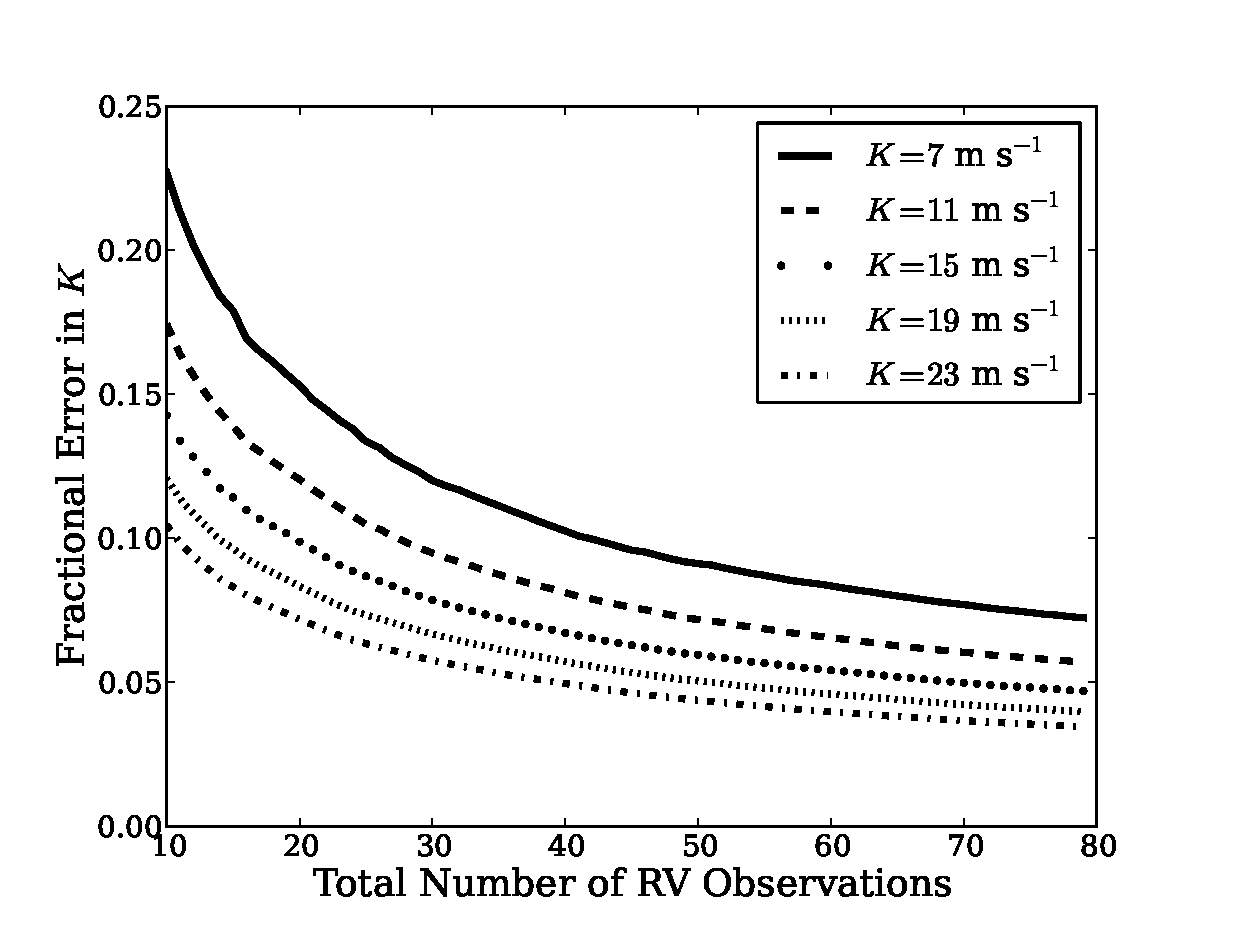
\includegraphics[width=0.75\textwidth]{chapter2/f1.eps}}
\caption[Simulated RV precision as a function of the number of
observations for specified Doppler semiamplitudes]{Derived fractional errors in the Doppler semiamplitude measurement as a function of number of radial velocity observations taken, for various values of $K$, the Doppler semiamplitude. For all observations, the same statistical uncertainties and RV jitter levels are assumed. The jitter level is 3 m/s, a reasonable estimate for all but the youngest dwarf stars. From top to bottom, these curves represent semiamplitudes of $[7, 11, 15, 19, 23]$ m/s. For a system like Kepler-18, where $K \approx 7$ m/s, many more measurements would be required to constrain $K$ to five percent (and thus the stellar mass to 15 percent). However, for a system with either larger planets or a smaller star, this level of precision could be reached with fewer observations.
  }

\label{RVerrors}
\end{figure}



\section{Summary and Discussion}

\label{S:SD}

We present a  method of measuring stellar and planetary masses dynamically by combining TTVs measured from transit light curves and follow-up radial velocity measurements. Our method can be used as an alternative to relying on stellar evolutionary models, which can be poorly constrained for non-solar type stars like M-dwarfs, subgiants, and F stars. By analyzing the Kepler-18 system and confirming our expressions with dynamical simulations of this system, we show the potential of our method.

While we show our method to be viable, especially for low-mass stars, using our method requires a somewhat specific set of circumstances. The system must contain two planets with masses large enough to force a detectable Doppler signal and observable transit timing variations on circular orbits near a first-order commensurability. \kep\ data suggests planets near resonance are common: more than 12 percent of planet systems show evidence for detectable transit timing variations \citep{Ford12a}, and dozens of planets near resonance have been confirmed through TTVs \citep{Steffen13}. Both the TTV and Doppler signals can be measured for super-Earth planets with periods less than 30 days; short-period systems such as these are extremely common \citep{Howard12}. Thus, it is likely that despite the specific requirements needed to use our system, it can be applied to a considerable number of \kep\ planetary systems.

As shown in Equations 14 and 15 of L12, the amplitude of the TTV signal is given such that
\begin{equation}
|V| \sim |V_\textrm{damped}|\bigg(1 + \frac{|Z_\textrm{free}|}{|\Delta|}\bigg),
\end{equation}
with $|V_\textrm{damped}|$ the amplitude of the TTV signal if the system were damped of its free eccentricity. The quantity $Z_\textrm{free}$ is defined such that $Z_\textrm{free} = f z_\textrm{free} + g z^\prime_\textrm{free}$, where $z$ is the complex eccentricity of the planet, $z = e\exp^{i \omega}$. Thus, our method as described will break down unless $|Z_{\textrm{free}}| \ll |\Delta|$. This is a resonable assumption for planets with periods under ten days. In theory, even if a non-negligible amount of free eccentricity remains in the system, a detailed radial velocity orbital solution could be used to calculate $Z_{\textrm{free}}$ and determine the system dynamical masses.

As a projection of the utility of this method, consider KOI 1241, a system containing two planets with periods of 10.5 and 21.4 days orbiting a giant star \citep[$R = 3.14 R_\odot$,][]{Steffen13}. There is evidence that this system has not dissipated all its free eccentricity, meaning it is not optimal for our study. However, with nine quarters of public \kep\ data, we can constrain the TTV signal caused by the larger planet in this system to 8.2 percent. Moreover, with only nine radial velocity observations, we can determine the radial velocity semiamplitude of the larger planet to 5.3 percent. Thus, from our method alone, if a system existed that was nearly identical to KOI 1241 but damped of free eccentricity, by Equations 11-13, we expect we could determine the stellar mass to 29 percent and the mass of the larger planet to within 22 percent. Our method could also be applied to KOI 1241 in the future if enough radial velocity data is collected to determine the magnitude of $Z_\textrm{free}$ for the system. The uncertainties in the TTV signal of KOI 1241 are larger than the uncertainty in the RV semiamplitude. The transit timing errors will decrease as more \kep\ data are released: decreasing the TTV error to five percent without including any additional radial velocity observations will reduce the uncertainty in the stellar mass to 20 percent. Thus our method could provide significant constraints on stellar masses in regimes where stellar atmospheres are less well-understood, such as subgiants and cool stars. For these cases, our method will be able to compliment asteroseismology results as an independent measure on the mass of the star. Moreover, our method can be used to find systems where the analytic stellar mass is substantially different than the Kepler Input Catalog values, which can then be followed up with dynamical modeling, asteroseismology, or high resolution spectroscopy to better characterize the star and orbiting planets.

With present data our technique is only viable as an alternative to stellar modeling in the most exceptional cases. Transit timing variations have been detected to remarkable precision by \textit{Kepler}, but very few KOIs have been followed up with radial velocity measurements. In the cases where RV data exists, only enough measurements were collected to confirm the planetary nature of the system, not to independently measure the planetary masses \citep{Holman10}. Our routine will become more useful for systems in which the RV semiamplitude can be better constrained. Additionally, the constraints provided by our technique can be applied as priors for model-grid interpolations of stellar masses. Thus these model-independent mass measurements can be used to guide and improve model-based stellar mass estimates.

Despite the faintness of the \kep\ planet candidate host stars, there are a few stars that would be ideal candidates for applications of our method. From the collection of Kepler Objects of Interest, we searched for stars hosting at least two transiting planets each with $P < 25$ days. We required at least one planet to be larger than 2 $R_\oplus$ and the planet periods to lie within five percent of a first-order mean-motion resonance. To ensure that all targets were optimized for radial velocity follow-up, we eliminated all targets fainter than $m_{\textrm{Kp}} = 13.0$. After making these cuts, we find 8 candidate systems to which this technique can be applied: KOI 85, 111, 115, 117, 244, 304, 1241 and 1930. As stated earlier in this section, KOI 1241 is not an ideal target because it has not been fully damped of its primordial eccentricity and there is not enough radial velocity information to uniquely determine the eccentricity of both planets. Of the remaining 7 systems, the CPS team has collected more than 10 radial velocity measurements only on one, KOI 244. Additional radial velocity measurements of any or all of the above systems would enable further validation of our procedure as well as additional constraints on the masses of each of the stars and their planets. Moreover, next-generation planet finding missions, such as TESS \citep{Brown08} and PLATO \citep{Catala10} will target bright stars, making detailed radial velocity follow-up observations of systems exhibiting transit timing variations a much more practical possibility. 

{\footnotesize
\begin{longtable}{lcccc} 
\hline
KOI & n & $t_n$ & TTV$_n$ & $\sigma_n$ \\
    &   & (BJD-2454900) & (d) & (d) \\
\hline
137.01 & 0 & 198.3142 & -0.0006 &  0.0012 \\
137.01 & 1 & 205.9557 &  0.0002 &  0.0013 \\
137.01 & 2 & 213.5973 &  0.0019 &  0.0018 \\
137.01 & 3 & 221.2389 &  0.0017 &  0.0010 \\
137.01 & 4 & 228.8804 &  0.0021 &  0.0017 \\
137.01 & 5 & 236.5220 &  0.0014 &  0.0015 \\
137.01 & 6 & 244.1636 &  0.0031 &  0.0011 \\
137.01 & 7 & 251.8052 &  0.0030 &  0.0011 \\
137.01 & 8 & 259.4467 &  0.0037 &  0.0012 \\
137.01 & 9 & 267.0883 &  0.0050 &  0.0012 \\
137.01 & 10 & 274.7299 &  0.0041 &  0.0012 \\
137.01 & 11 & 282.3714 &  0.0037 &  0.0018 \\
137.01 & 12 & 290.0130 &  0.0035 &  0.0018 \\
137.01 & 13 & 297.6546 &  0.0028 &  0.0012 \\
137.01 & 14 & 305.2961 &  0.0034 &  0.0011 \\
137.01 & 15 & 312.9377 &  0.0026 &  0.0011 \\
137.01 & 16 & 320.5793 &  0.0013 &  0.0011 \\
137.01 & 17 & 328.2209 &  0.0018 &  0.0012 \\
137.01 & 18 & 335.8624 &  0.0008 &  0.0015 \\
137.01 & 20 & 351.1456 &  0.0001 &  0.0011 \\
137.01 & 21 & 358.7871 & -0.0005 &  0.0012 \\
137.01 & 22 & 366.4287 & -0.0027 &  0.0014 \\
137.01 & 23 & 374.0703 & -0.0033 &  0.0014 \\
137.01 & 24 & 381.7119 & -0.0024 &  0.0011 \\
137.01 & 25 & 389.3534 & -0.0025 &  0.0011 \\
137.01 & 26 & 396.9950 & -0.0033 &  0.0011 \\
137.01 & 27 & 404.6366 & -0.0036 &  0.0013 \\
137.01 & 28 & 412.2781 & -0.0046 &  0.0012 \\
137.01 & 29 & 419.9197 & -0.0037 &  0.0011 \\
137.01 & 30 & 427.5613 & -0.0038 &  0.0015 \\
137.01 & 31 & 435.2028 & -0.0039 &  0.0013 \\
137.01 & 32 & 442.8444 & -0.0019 &  0.0012 \\
137.01 & 33 & 450.4860 & -0.0013 &  0.0011 \\
137.01 & 34 & 458.1276 & -0.0017 &  0.0010 \\
137.01 & 35 & 465.7691 & -0.0008 &  0.0015 \\
137.01 & 36 & 473.4107 &  0.0005 &  0.0013 \\
137.01 & 37 & 481.0523 &  0.0016 &  0.0011 \\
137.01 & 38 & 488.6938 &  0.0026 &  0.0014 \\
137.01 & 39 & 496.3354 &  0.0027 &  0.0015 \\
137.01 & 40 & 503.9770 &  0.0030 &  0.0014 \\
137.01 & 41 & 511.6186 &  0.0038 &  0.0011 \\
137.01 & 42 & 519.2601 &  0.0032 &  0.0013 \\
137.01 & 43 & 526.9017 &  0.0052 &  0.0013 \\
137.01 & 44 & 534.5433 &  0.0055 &  0.0013 \\
137.01 & 45 & 542.1848 &  0.0034 &  0.0010 \\
137.01 & 46 & 549.8264 &  0.0025 &  0.0014 \\
137.01 & 47 & 557.4680 &  0.0049 &  0.0021 \\
137.01 & 48 & 565.1095 &  0.0035 &  0.0011 \\
137.01 & 49 & 572.7511 &  0.0030 &  0.0012 \\
137.01 & 50 & 580.3927 &  0.0017 &  0.0010 \\
137.01 & 51 & 588.0343 &  0.0034 &  0.0016 \\
137.01 & 52 & 595.6758 &  0.0013 &  0.0011 \\
137.01 & 54 & 610.9590 & -0.0006 &  0.0012 \\
137.01 & 55 & 618.6005 & -0.0019 &  0.0012 \\
137.01 & 56 & 626.2421 & -0.0015 &  0.0016 \\
137.01 & 57 & 633.8837 & -0.0026 &  0.0012 \\
137.01 & 58 & 641.5253 & -0.0016 &  0.0012 \\
137.01 & 61 & 664.4500 & -0.0046 &  0.0014 \\
137.01 & 62 & 672.0915 & -0.0028 &  0.0012 \\
137.01 & 63 & 679.7331 & -0.0042 &  0.0012 \\
137.01 & 65 & 695.0162 & -0.0032 &  0.0011 \\
137.01 & 66 & 702.6578 & -0.0025 &  0.0013 \\
137.01 & 67 & 710.2994 & -0.0029 &  0.0012 \\
137.01 & 68 & 717.9410 & -0.0029 &  0.0011 \\
137.01 & 69 & 725.5825 & -0.0004 &  0.0013 \\
137.01 & 71 & 740.8657 &  0.0006 &  0.0013 \\
137.01 & 72 & 748.5072 &  0.0006 &  0.0014 \\
137.01 & 73 & 756.1488 &  0.0014 &  0.0011 \\
137.01 & 74 & 763.7904 &  0.0049 &  0.0017 \\
137.01 & 75 & 771.4320 &  0.0011 &  0.0016 \\
137.01 & 76 & 779.0735 &  0.0033 &  0.0012 \\
137.01 & 77 & 786.7151 &  0.0021 &  0.0011 \\
137.01 & 78 & 794.3567 &  0.0031 &  0.0012 \\
137.01 & 79 & 801.9982 &  0.0039 &  0.0012 \\
137.01 & 80 & 809.6398 &  0.0029 &  0.0014 \\
137.01 & 81 & 817.2814 &  0.0038 &  0.0011 \\
137.01 & 82 & 824.9229 &  0.0016 &  0.0012 \\
137.02 & 0 & 194.8832 &  0.0000 &  0.0010 \\
137.02 & 1 & 209.7421 & -0.0012 &  0.0011 \\
137.02 & 2 & 224.6011 & -0.0025 &  0.0010 \\
137.02 & 3 & 239.4600 & -0.0037 &  0.0010 \\
137.02 & 4 & 254.3189 & -0.0029 &  0.0010 \\
137.02 & 6 & 284.0368 & -0.0032 &  0.0011 \\
137.02 & 7 & 298.8958 & -0.0040 &  0.0011 \\
137.02 & 8 & 313.7547 & -0.0013 &  0.0010 \\
137.02 & 9 & 328.6136 & -0.0023 &  0.0023 \\
137.02 & 10 & 343.4726 & -0.0005 &  0.0011 \\
137.02 & 11 & 358.3315 &  0.0008 &  0.0009 \\
137.02 & 12 & 373.1905 &  0.0017 &  0.0012 \\
137.02 & 13 & 388.0494 &  0.0036 &  0.0010 \\
137.02 & 14 & 402.9083 &  0.0029 &  0.0011 \\
137.02 & 15 & 417.7673 &  0.0020 &  0.0010 \\
137.02 & 16 & 432.6262 &  0.0008 &  0.0012 \\
137.02 & 17 & 447.4852 &  0.0008 &  0.0011 \\
137.02 & 18 & 462.3441 &  0.0008 &  0.0011 \\
137.02 & 19 & 477.2030 & -0.0001 &  0.0011 \\
137.02 & 20 & 492.0620 &  0.0002 &  0.0010 \\
137.02 & 21 & 506.9209 & -0.0023 &  0.0011 \\
137.02 & 22 & 521.7799 & -0.0024 &  0.0010 \\
137.02 & 23 & 536.6388 & -0.0038 &  0.0010 \\
137.02 & 24 & 551.4977 & -0.0035 &  0.0010 \\
137.02 & 25 & 566.3567 & -0.0033 &  0.0011 \\
137.02 & 26 & 581.2156 & -0.0033 &  0.0010 \\
137.02 & 27 & 596.0746 & -0.0013 &  0.0015 \\
137.02 & 29 & 625.7924 &  0.0020 &  0.0010 \\
137.02 & 31 & 655.5103 &  0.0032 &  0.0014 \\
137.02 & 32 & 670.3693 &  0.0015 &  0.0011 \\
137.02 & 33 & 685.2282 &  0.0026 &  0.0009 \\
137.02 & 34 & 700.0871 & -0.0011 &  0.0011 \\
137.02 & 35 & 714.9461 &  0.0008 &  0.0010 \\
137.02 & 36 & 729.8050 & -0.0019 &  0.0010 \\
137.02 & 37 & 744.6640 & -0.0012 &  0.0011 \\
137.02 & 38 & 759.5229 & -0.0027 &  0.0011 \\
137.02 & 39 & 774.3818 & -0.0030 &  0.0012 \\
137.02 & 40 & 789.2408 & -0.0034 &  0.0010 \\
137.02 & 41 & 804.0997 & -0.0052 &  0.0010 \\
137.02 & 42 & 818.9587 &  0.0003 &  0.0013 \\
\hline
\caption{Transit times for \kep\ transiting planet candidates
in the KOI-137 system}
\label{TTTable}
\end{longtable}
}




\chapter{The Occurrence Rate of Giant Planets around M Dwarfs}
\label{chap:trends}

In this chapter I develop a method to determine the occurrence
rate of giant planets in wide orbits around their host stars.
These planets are large enough to cause a slow drift, or trend, in 
the RV of their host star, but too distant from their star to
observe the full orbit on a reasonable timescale.
Such a trend could be caused by a planet, or a star on a much
wider orbit. As stars would be easily observable with high-contrast
direct imaging, the existence of a trend combined with an AO 
non-detection suggests the presence of a planet is likely.
The definitive presence of any single planet can not be 
determined, but by analyzing a population of these systems their
bulk occurrence can be measured.
This chapter was originally published as ``The TRENDS High-contrast Imaging Survey. IV. The Occurrence Rate of Giant Planets around M Dwarfs,'' ApJ, 781, 28 (2014) by BTM, Justin Crepp, John Johnson,
Andrew Howard, and Geoff Marcy. 


\section{Introduction}

Over the past twenty years, numerous planets have been detected by several different techniques, permitting the first estimates of the occurrence rate of planets orbiting stars in the solar neighborhood \citep[e.g.][]{Johnson10b, Howard10b, Gould10, Vigan12}. As successful as these detection methods have been, each is sensitive only to a relatively narrow range of parameter space. For example, radial velocity (RV) studies are most sensitive to massive planets with orbital periods shorter than the time baseline of observations. %For example, 
% \citet{Wright12} calculate that $1.20\% \pm 0.38\%$ of FGK stars host a ``hot Jupiter'' with mass larger than $m \sin i > 0.1 M_J$ and period shorter than 10 days. By analyzing stars with longer period RV signals,
\citet{Johnson10b} find that $3.4^{+2.2}_{-0.9}\%$ of M dwarfs have a Saturn-mass or larger planet within 2.5 AU. Beyond a few AU, RV searches are incomplete as the time required for a planet to complete one orbit is longer than the typical observing baseline. Some studies have attempted to extrapolate beyond this boundary. For instance, \citet{Cumming08} fit the observed RV planet population to a power law in planet mass and period and find that $18\% \pm 1\%$ of FGK stars host a Saturn-mass or larger planet within 20 AU. Recently, targeted RV surveys of M-dwarfs have suggested the giant planet occurrence rate is significantly smaller for these diminutive stars. \citet{Bonfils13} suggest fewer than $1\%$ of M-dwarfs host a Saturn-mass or larger planet with an orbital period $1 < P < 10$ days, and $2^{+3}_{-1}\%$ host giant planets with orbital periods between 10 and 100 days.

Transit studies suffer from similar detection biases. Since a planet transits only once each orbit, several orbits must be observed to definitively confirm a planet so characterization is limited to planets with periods shorter than a fraction of the observing baseline \citep{Gaudi05}. Additionally, the probability of a planet transiting its host star decreases with increasing orbital period \citep{Winn11}, such that hundreds of thousands of stars must be monitored in order to study the planet population at $a \approx 1$ AU \citep{Borucki84}. Nevertheless, the success of the \textit{Kepler} mission \citep{Borucki10, Koch10} has allowed for statistical analyses of transiting planets to be undertaken. For example, \citet{Morton14} analyze M dwarfs included in the 2012 list of announced Kepler Objects of Interest \citep[KOIs,][]{Batalha13}. By correcting for false positives (detections when no transiting planet exists), false negatives (nondetections when a transiting planet is present) and geometric effects (nondetections of nontransiting planets), they estimate an occurrence rate of $1.5$ planets with periods less than 90 days and radii larger than $0.5R_\oplus$ per M dwarf star. The occurrence rate found by these authors is slightly higher than previous analyses which measure rates of approximately one planet per star \citep{Youdin11, Mann12, Swift13, Dressing13}.

Neither RV nor transit searches are yet conducive to the discovery and characterization of planets well beyond the ``snow line,'' where water exists as ice. Instead, high contrast direct imaging techniques can be a powerful tool for detecting young planetary companions in this domain. The first direct imaging planet discoveries are securely in hand, including four companions to HR\,8799 \citep{Marois08, Marois10} and one each around $\beta$ Pictoris \citep{Lagrange09}, and Gl\,504 \citep{Kuzuhara13}\footnote{Companions detected around Fomalhaut \citep{Kalas08, Currie12}, HD 95086 \citep{Rameau13}, and LaCa15 \citep{Kraus12} are also good candidates to be directly imaged planets, but their true nature is somewhat ambiguous.}. Recent studies using these techniques have calculated an occurrence rate around A stars of $8.7^{+10.1}_{-2.8}\%$ at $1\sigma$ confidence for planets larger than $3 M_J$ and separations between 5 and $320 \textrm{ AU}$ \citep{Vigan12}. Imaging studies have been most effective around high mass stars. \citep{Crepp11, Carson13}. Nondetections around lower-mass stars have been used to place upper limits on the frequency of giant planets. For example, \citet{Nielsen10} rule out the presence of giant planets orbiting FGKM stars beyond 65 AU with $95\%$ confidence. High contrast imaging, while powerful, only provides a measure of the relative brightness of a companion. To estimate the companion's mass, the age of the star must be known and planetary thermal evolution models must be applied to estimate the temperature (and brightness) of the companion \citep{Chabrier00, Baraffe03}. Moreover, direct imaging is currently only sensitive to massive planets; the HR8799 planets and $\beta$ Pic b are believed to have masses $m > 5 M_J$. RV and transit studies suggest such ``super-Jupiters'' are rare compared to Jovian-mass and smaller objects at smaller separations \citep{Howard10b, Howard12}.

The gravitational microlensing technique is also effective for finding giant planets in wide orbits and does not rely on planetary evolution models. Using this technique, planets can be detected by observing perturbations to the photometric gravitational microlensing signal when a planet and its host pass in front of a more distant star. Since $70-75\%$ of stars in the galaxy are M-dwarfs, most lenses have mass $M < 0.5 M_\odot$. Microlensing searches thus provide a measure of planet occurrence around low mass stars. Microlensing studies are sensitive to planets near the Einstein ring, $R_E \sim 3.5 \mbox{AU} (M/M_\odot)^{1/2}$, a much wider separation than RV and transit searches \citet{Gould10}. \citet{Cassan12} find microlensing searches are most sensitive to planets at a projected separation in the range $[s_{\textrm{max}}^{-1}R_E, s_{\textrm{max}}R_E]$, where $s_{\textrm{max}} \sim (q/10^{-4.3})^{1/3}$ and $q$ is the mass ratio between a companion and the host star. These authors find a planet occurrence rate that can be parameterized by a double power-law function, in mass ratio $q$ and separation $s$, such that
\begin{equation}
\frac{d^2N}{d\log q d \log s} = 10^{-0.62 \pm 0.22} \bigg(\frac{q}{5 \times 10^{-4}}\bigg)^{-0.73 \pm 0.17} \mbox{dex}^{-2}.
\label{microlensingresults}
\end{equation}
The normalization constant is equivalent to $0.24^{+0.16}_{-0.10}$. These results are calculated under the assumption that planets are distributed uniformly in $\log s$, as is the case for binary stars \citep{Opik24}. Additionally, \citet{Sumi10} find a power-law slope in mass such that $dN/ d\log q \propto q^{-0.68 \pm 0.20}$ for Neptune-sized planets, but do not attempt to quantify a normalization factor. 

As microlensing studies focus on distant M-dwarfs ($d > 1$ kpc) in the direction of the galactic bulge \citep{Gaudi02}, these stars can be difficult to characterize accurately due to crowding. Stellar masses and metallicities are often estimated without being measured spectroscopically. If these host stars have different masses than assumed, it would affect the results of planet occurrence rate studies by microlensing groups as microlensing results do not account for correlations between stellar and planet properties. Additionally, as microlensing searches are most sensitive near $r = R_E$, beyond approximately 10 AU the lensing signal becomes very weak, and differentiating distant planets from unbound, ``free-floating'' planets becomes difficult \citep{Sumi11}.

RV and microlensing studies probe different regions around a star, and extrapolations between the two domains suggest a possible discrepancy. \citet{Cassan12} estimate a total giant planet occurrence rate significantly lower than the \citet{Cumming08} RV result.
% studied the statistics of the Keck/HIRES Doppler survey and found that $18 \pm 1 \%$ of FGK dwarfs have a planet at least as massive as Saturn within 20 AU, lower than the predictions offered by microlensing results. 
Derived power-law distributions in mass may also be different for planets found by each method: \citet{Cumming08} find a distribution such that $dN/d \log m \propto m^{-0.31 \pm 0.20}$ from RV-detected planets, while \citet{Cassan12} find a distribution such that $dN/ d\log q \propto q^{-0.73 \pm 0.17}$. Since microlensing studies target M-dwarfs, which are confined to a narrow mass range, we can approximate $q = m/M$ as $m$. In this case, the microlensing result and RV result differ by $1.6 \sigma$.  Since giant planet occurrence decreases with decreasing stellar mass and metallicity \citep{Johnson10a}, the expected giant planet occurrence rate around M dwarfs would be smaller than that for FGK stars. Therefore, it is necessary to compare the microlensing planet population not to a population of FGK stars, but instead to a study of RV detected planets around M-dwarfs.

Historically, RV observations have been used to detect and characterize planets once they complete a full orbit, limiting studies to planets with periods shorter than the observing time baseline. In this paradigm, potentially useful information is overlooked. Wide companions are not completely undetectable: instead they can be identified by the presence of long-term RV accelerations (linear ``trends'')  which can be used to infer the existence of a companion in a more distant orbit \citep{Liu02, Crepp12a}. However, a linear acceleration does not provide unique information about the mass and period of the companion: the same trend could be caused by a Jupiter-mass planet at 5 AU or a $100 M_J$ M-dwarf at 25 AU. This degeneracy can be broken by adaptive optics (AO) imaging. Low-mass binary companions to nearby M-dwarfs can be easily imaged by modern AO systems \citep{Lloyd02, Siegler03}. Such detections form the basis for the TRENDS High-Contrast Imaging Survey, which to date has detected four M-dwarfs and one white dwarf companion to higher mass stars\citep{Crepp12b, Crepp13a, Crepp13b}.

In this work, we combine RV and AO observations of nearby cool stars to estimate the frequency of giant planets in wide orbits around M-dwarfs. From a sample of 111 M-dwarfs observed with a median Doppler RV baseline of 11.8 years, we identify 4 systems with long-term RV accelerations but no known companions and target these stars with AO imaging in an attempt to detect stellar-mass companions. We discuss these observations and our methodology in \textsection\ref{SO}. Given an observed RV trend or lack thereof, we determine with high statistical confidence if a giant planet exists around each star. We analyze the effects of false positive and false negative detections of RV accelerations in our sample in \textsection\ref{Stats}. In \textsection\ref{Results} we estimate the occurrence rate of giant planets around M-dwarfs and compare the measure to results from other techniques. We summarize and conclude in \textsection\ref{SC}, and 
provide notes about individual targets in \textsection 6.
In \textsection 7, we include a brief note about magnetic activity.

 This study represents the first measurement of the planet population in the range 0--20 AU. While we rely on brown dwarf cooling models, our study does not make use of theoretical planetary evolution models, unlike other AO studies of planetary systems.

\section{Sample and Observations}
\label{SO}
\subsection{Target Selection}
\label{TS}

Since 1997, the California Planet Search (CPS) collaboration has undertaken a comprehensive Doppler search for extrasolar planets at the Keck Observatory \citep[e.g. ][]{Howard10}. Using Keck/HIRES \citep{Vogt94}, the CPS program monitors over 2000 stars, most selected to be chromospherically quiet, single, and bright. Included in this sample is a collection of M-dwarfs from the Gliese and Hipparcos catalogs brighter than $V = 11.5$ and lacking known stellar companions within 2 arcseconds \citep{Rauscher06}. This sample was later extended to $V = 13.5$ and currently includes 131 M-dwarfs within 16 pc of the Sun, where we define the M spectral class as targets with $B-V > 1.44$.

To develop the sample used here, we first remove from this set 16 stars with a known, nearby stellar binary companion. We define ``nearby'' as a separation small enough that a test particle orbit with semimajor axis $\geq 30$ AU would be unstable, following the instability criterion of \citet{Holman99}. This criterion depends on the unknown eccentricity of the binary pair, as perturbative effects are maximized at periapsis. We take $e=0.5$ as a typical value and find the onset of instability occurs for binary stars with $a \sim 250$ AU. Planets can still form in these more compact binary systems \citep[e.g. Gl667C; ][]{Anglada-Escude12b} but at such small separations protoplanetary disk formation and planet evolution would be affected significantly by the presence of stellar companions. This selection thus allows us to study a class of planets that likely followed similar evolutionary processes. Moreover, the detection of an acceleration around these stars is ambiguous, as it could be caused by the binary star, a planetary-mass companion, or both together.

After making the above selection we are left with 111 RV targets, all of which have at least 8 radial velocity observations and a time baseline longer than 2.9 years. The median number of observations is 29 over a median time baseline of 11.8 years. The stars have spectral types from M0 to M5.5 and masses in the range $0.64M_\odot - 0.10M_\odot$. Stellar masses are estimated using the empirical relation between mass and absolute K-band magnitude, $M_K$, described by \citet{Delfosse00}. We take $10\%$ as a typical uncertainty in the stellar mass, in line with previous estimates \citep{Bean06}. $K$-band apparent magnitudes are measured using apparent magnitudes from the 2MASS point-source catalog \citep{Cutri03}. The majority of our parallaxes are taken from an analysis of \textit{Hipparcos} data \citep{vanLeeuwen07}. Some of our stars were not observed by Hipparcos, while others have had their distances updated more recently. In these cases, we apply the distances listed in the SIMBAD astronomical database (Table \ref{T1}). For example, for Gl\,317 we use the parallax found by \citet{Anglada-Escude12a}; their derived mass and metallicity are consistent with our estimated values. In all cases, stellar metallicities are estimated by measuring the offset between the star's position in the \{$V-K_s, M_{K_S}$\} plane from a calibrated main sequence following the method of \citet{Neves12}. We take 0.17 dex as a typical uncertainty in the stellar metallicity, representative of the scatter between this photometric method and spectroscopic measures of stellar metallicity. Stellar parameters for these targets are listed in Table \ref{T1} and observational parameters are listed in Table \ref{T1b}. The distribution of RV observational parameters are shown in Figure \ref{Hists}. Spectral types are estimated by comparing the spectrum collected with HIRES to other spectra collected with this same instrument. RV observations for a representative sample of six ``typical'' stars are shown in Figure \ref{RVfig}. 

\begin{figure}[htbp]
\centerline{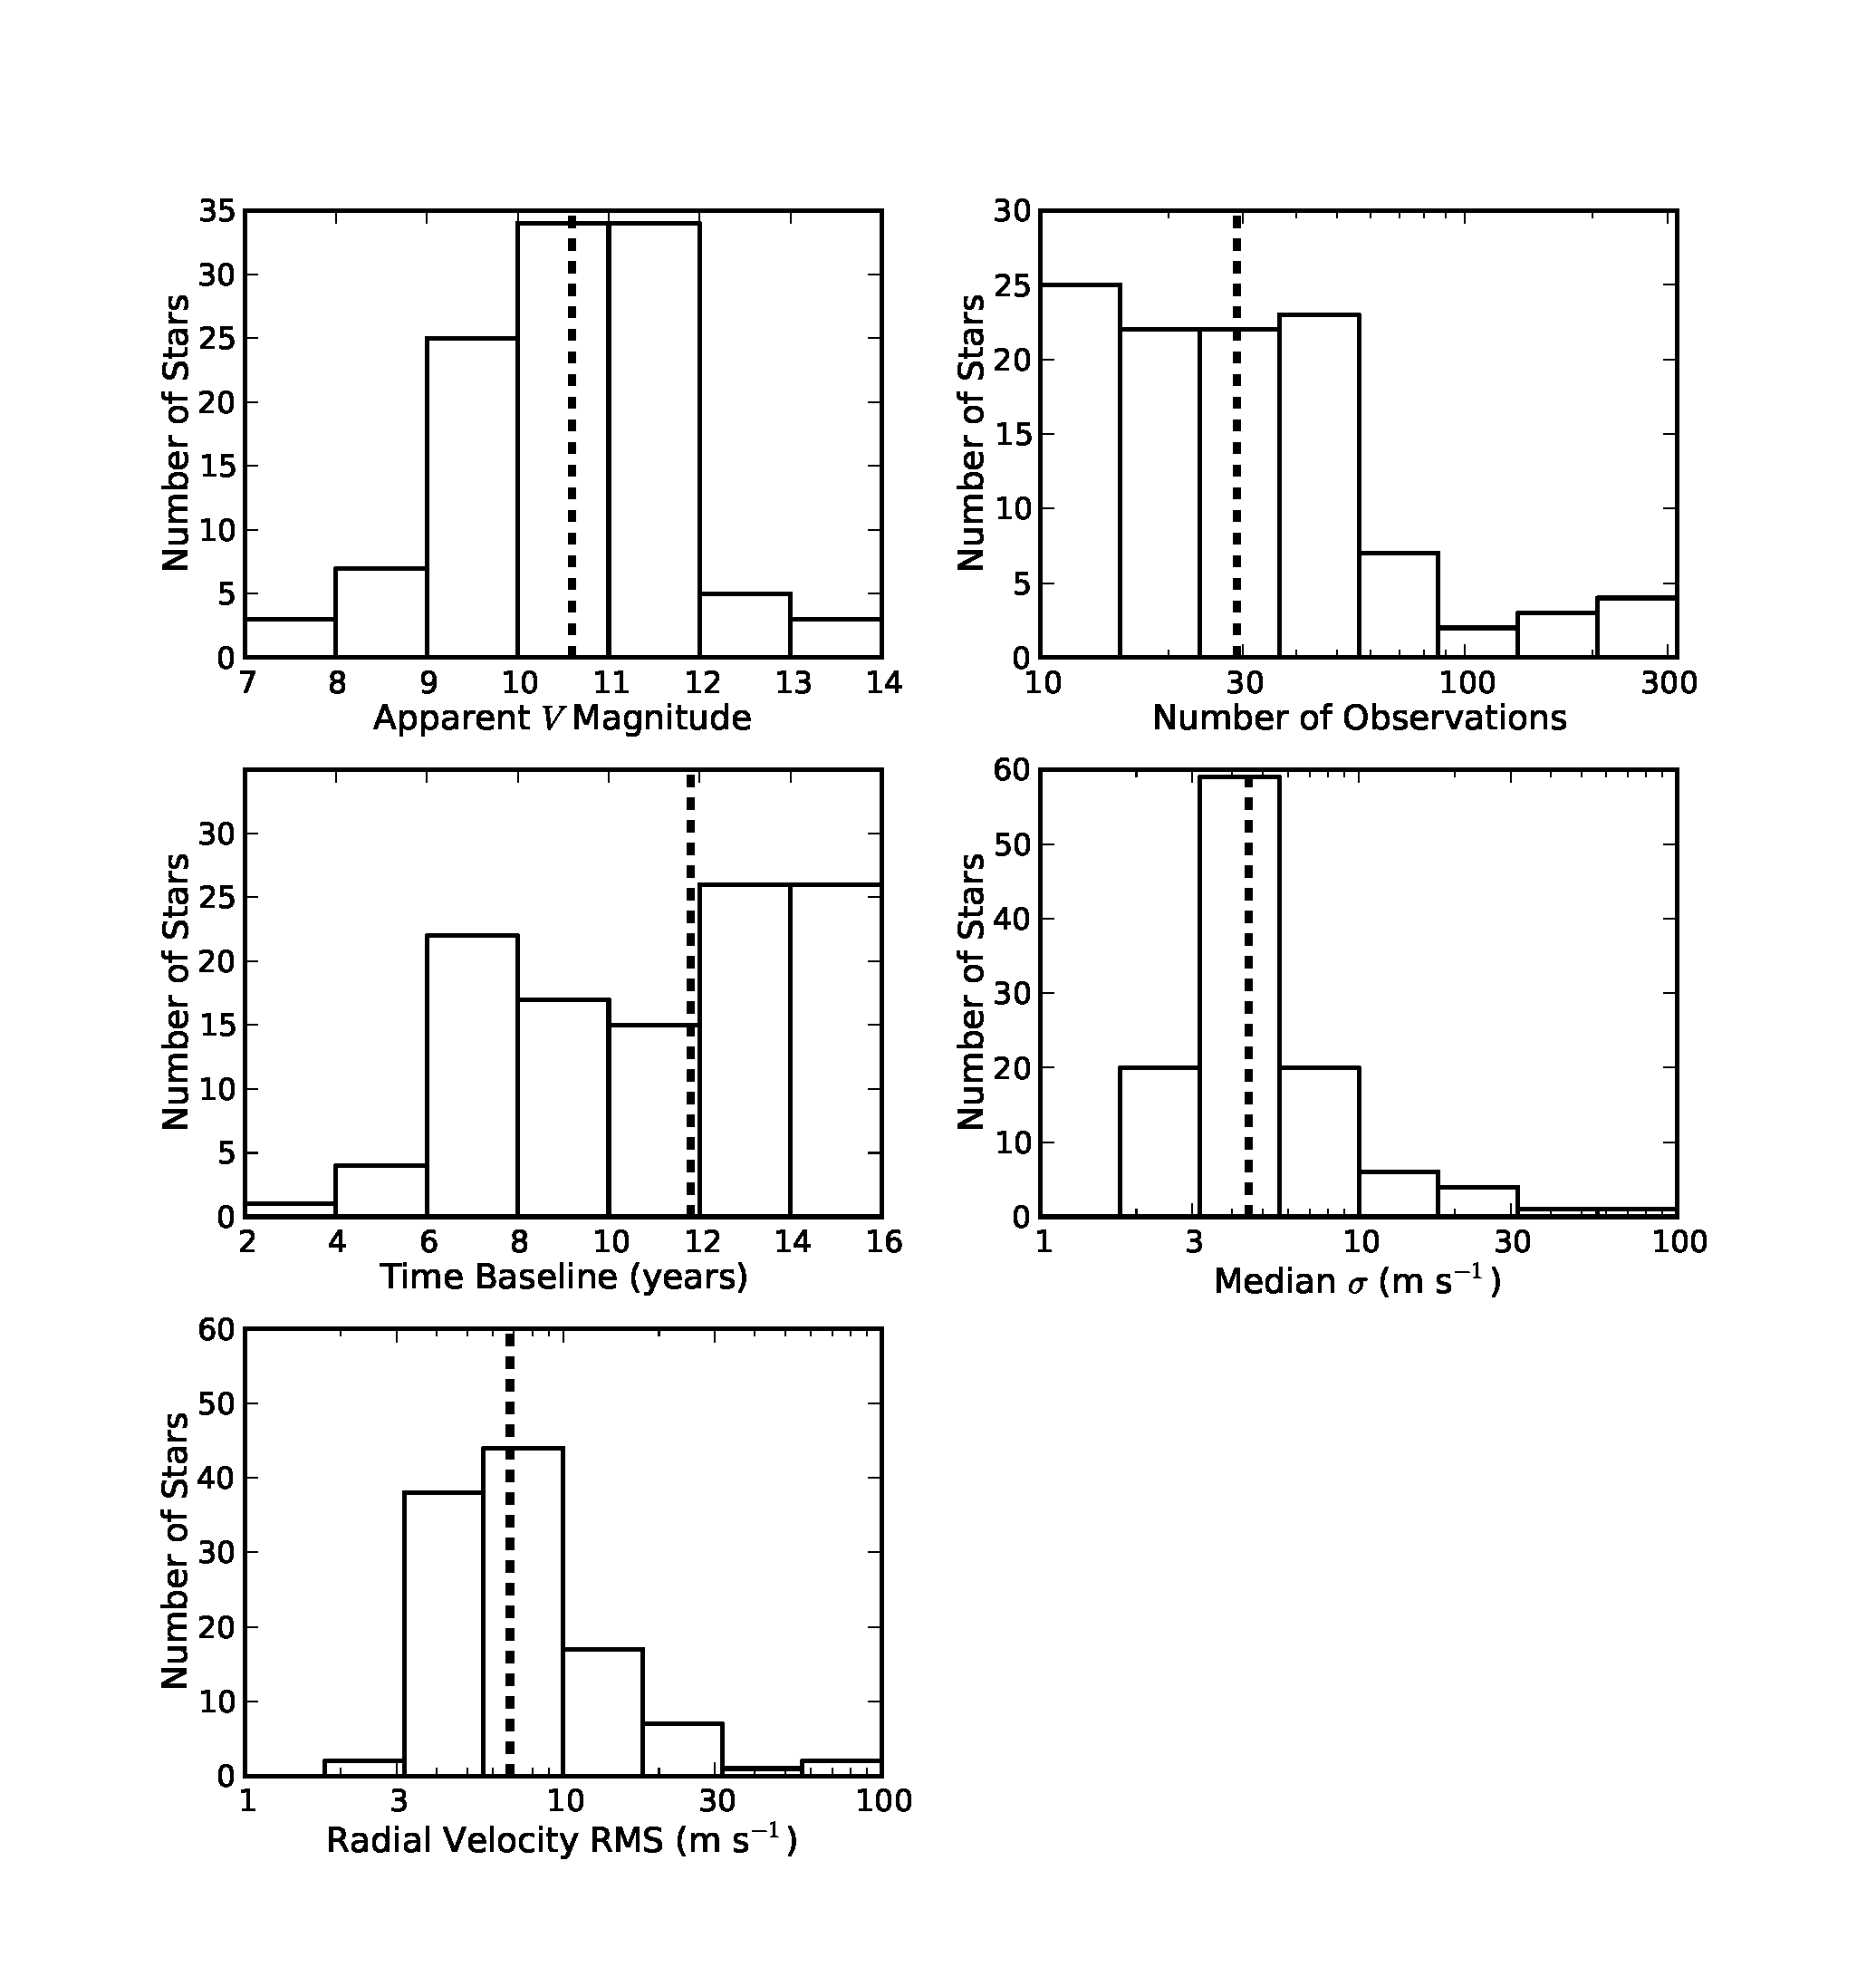
\includegraphics[width=1.0\textwidth]{chapter3/f1.eps}}
\caption[Summary statistics of RV observations]{Distributions of the RV observational parameters. Dashed lines represent the median values for each parameter. The median target brightness is $V = 10.6$, and the median target has been observed 29 times over 11.8 years. The median measurement uncertainty $\sigma$, defined as the sum in quadrature of rotational jitter and statistical uncertainty (Eq. \ref{sigmaeq}) is 4.5 m s$^{-1}$. Specific parameters for each individual system are shown in Table \ref{T1}.
  }
\label{Hists}
\end{figure}


\begin{figure}[htbp]
\centerline{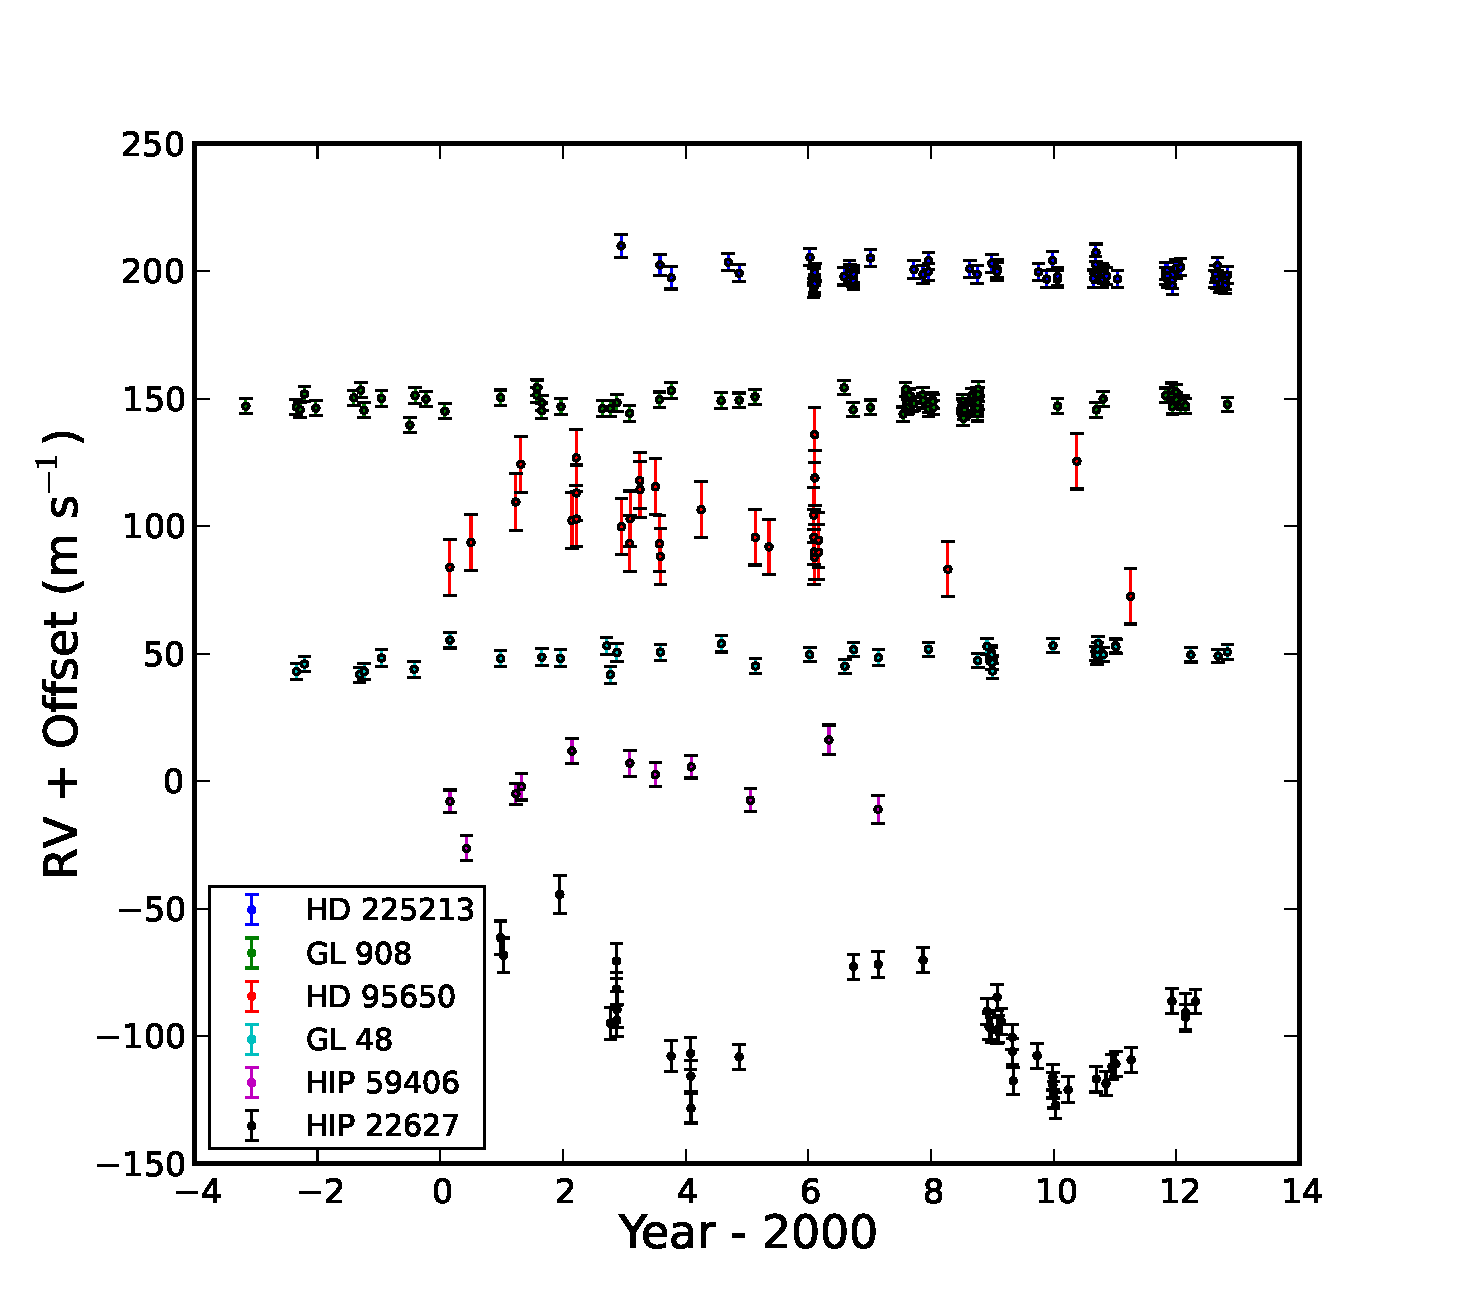
\includegraphics[width=0.75\textwidth]{chapter3/f2.eps}}
\caption[RV measurements for a representative sample of six example stars]{RV measurements for a representative sample of six example stars. The stars are arranged such that the brightest star is at the top of the plot. The individual stars vary considerably with respect to observing baselines, measurement uncertainty, and number of observations. Of these stars, HIP\,59406 has a wide binary companion, while HIP\,22627 has both a known inner planet and long-term RV acceleration.
  }
\label{RVfig}
\end{figure}

\subsection{Detecting Accelerations from Radial Velocities}
\label{RVs}

The detection of a long-term RV acceleration is facilitated by having many observations over a long time baseline to increase signal, but complicated by astrophysical ``jitter'' caused by rotational modulation of surface inhomogeneties. To determine the masses and semimajor axes to which we are sensitive to planetary companions, we inject a series of artificial companions into orbit around the stars in our sample. We define a logarithmically spaced grid of companion masses and semimajor axes spanning the range $0.75 M_J < m < 100 M_J$ and $3 \textrm{AU} < a < 30 \textrm{AU}$, such as the one shown in Figure \ref{Detectability}. At each point, we inject 500 planets and randomly assign each of the remaining orbital elements. The longitude of ascending node $\Omega$, time of periapsis $t_p$, and argument of periapsis $\omega$ are drawn from a uniform distribution, while the inclination is drawn from a distribution $dn/di = \sin i$ and the eccentricity from a distribution such that $dn/de$ follows a beta distribution with $a = 1.12$ and $b = 3.09$, which well-replicates the distribution of observed eccentricities for RV planets with orbits longer than 382 days \citep{Kipping13}. We then numerically integrate these orbits forward in time over our true observing baseline. 



At the epochs each star was observed by CPS, we calculate the expected radial velocity signal caused by our injected planet. Each velocity is perturbed from the true expected Keplerian velocity by a normal variate with zero mean and standard deviation $\sigma$ representative of the total expected noise:
\begin{equation}
\sigma = \sqrt{\sigma_\gamma^2 + \sigma^2_\textrm{jitter}}.
\label{sigmaeq}
\end{equation}
Here, $\sigma_\gamma$ is the photon noise, estimated for each individual observation by randomly selecting a single measurement of the measured Poisson photon noise from a true observation of the star. To account for the effects of jitter, we follow the method of \citet{Isaacson10}, who develop an empirical relation between the level of stellar jitter, a star's $S_{\textrm HK}$ value, and its $B-V$ color. $S_{\textrm HK}$ is defined as the ratio of the flux in the Ca II line cores to flux in the surrounding continuum. We compare the $S_{HK}$ value observed by CPS to that expected from the star's $B-V$ color, which provides an estimate of $\sigma_\textrm{jitter}$. This value is added in quadrature to the photon noise to estimate a total observational uncertainty, $\sigma$. Typical observations carry a photon noise of $2-4$ m s$^{-1}$ and jitter values are typically $3-5$ m s$^{-1}$ for a total $\sigma$ value of $3-6$ m s$^{-1}$ for the majority of stars. Median $\sigma$ values for each star are listed in Table 2.

Once all observations are accounted for, we search for evidence of our injected planetary companion, manifested as an acceleration in the RV data. Here, we define the existence of a trend using the Bayesian Information Criterion \citep[BIC;][]{Schwarz78, Bowler10, Campo11, Stevenson12}, which prefers simple, well-fitting models subject to 
\begin{equation}
\textrm{BIC} \equiv -2 \ln \mathcal{L} + k \ln N,
\label{EqBIC}
\end{equation}  
where $\mathcal{L}$ is the maximum likelihood for a model with $k$ free parameters and $N$ observations. The BIC thus favors models that fit the underlying data well, but penalizes increasingly complex models. For a more complex model to be preferred by the BIC, it must improve the fit by an amount greater than $k \ln N$ to overcome the penalty term.

\citet{Kass95} claim a difference between BIC values provides a bounded approximation of twice the logarithm of the Bayes factor. A change in BIC value of ten or more (corresponding to a Bayes factor of approximately 0.01) suggests strong evidence for an association between two parameters. If the BIC value decreases by more than 10 when considering a model with a linear acceleration over a model with only an offset, a planet is considered to be detected. Otherwise, the system is considered a non-detection. We find that the $\Delta$BIC value chosen here is consistent with by-eye inspection of our data in a visual search for RV accelerations. In both cases, we allow for a linear offset in the RV data in August, 2004, corresponding to an upgrade of the HIRES CCD detector \citep{Wright11}. Effectively, we treat the data from before and after the upgrade as coming from two distinct instruments, which serves to slightly decrease our sensitivity to small RV accelerations.

By repeating this process for many simulated planets over our mass-semimajor axis grid, we can map out the relative probability of detecting a linear trend caused by a planet as a function of companion mass and semimajor axis. As an example, Figure \ref{Detectability} shows RVs for HIP\,70975 and the likelihood of detecting a planet at a given mass and period given these observations. Figure \ref{DetectFull} shows the mean likelihood of detecting a planet around a given star across our sample. Throughout this work, we report the occurrence rate of planets with masses in the range $1 M_J < m < 13 M_J$. We can detect accelerations caused by planets smaller than $1 M_J$ in certain instances, but would miss the majority of these planets. As Figure \ref{DetectFull} shows, we can only detect a $0.75 M_J$ planet at 6 AU $50\%$ of the time; planets at smaller separations would exhibit significant curvature over a 12 year time baseline and could be detected through an RV survey alone. We are more efficient at detecting planets larger than $1 M_J$, although we would still not expect to detect all planets in this range. We account for false negative ``missed'' planets in our analysis, as described in \textsection\ref{FN}.




\begin{figure}[htbp]
        \centering      
\centerline{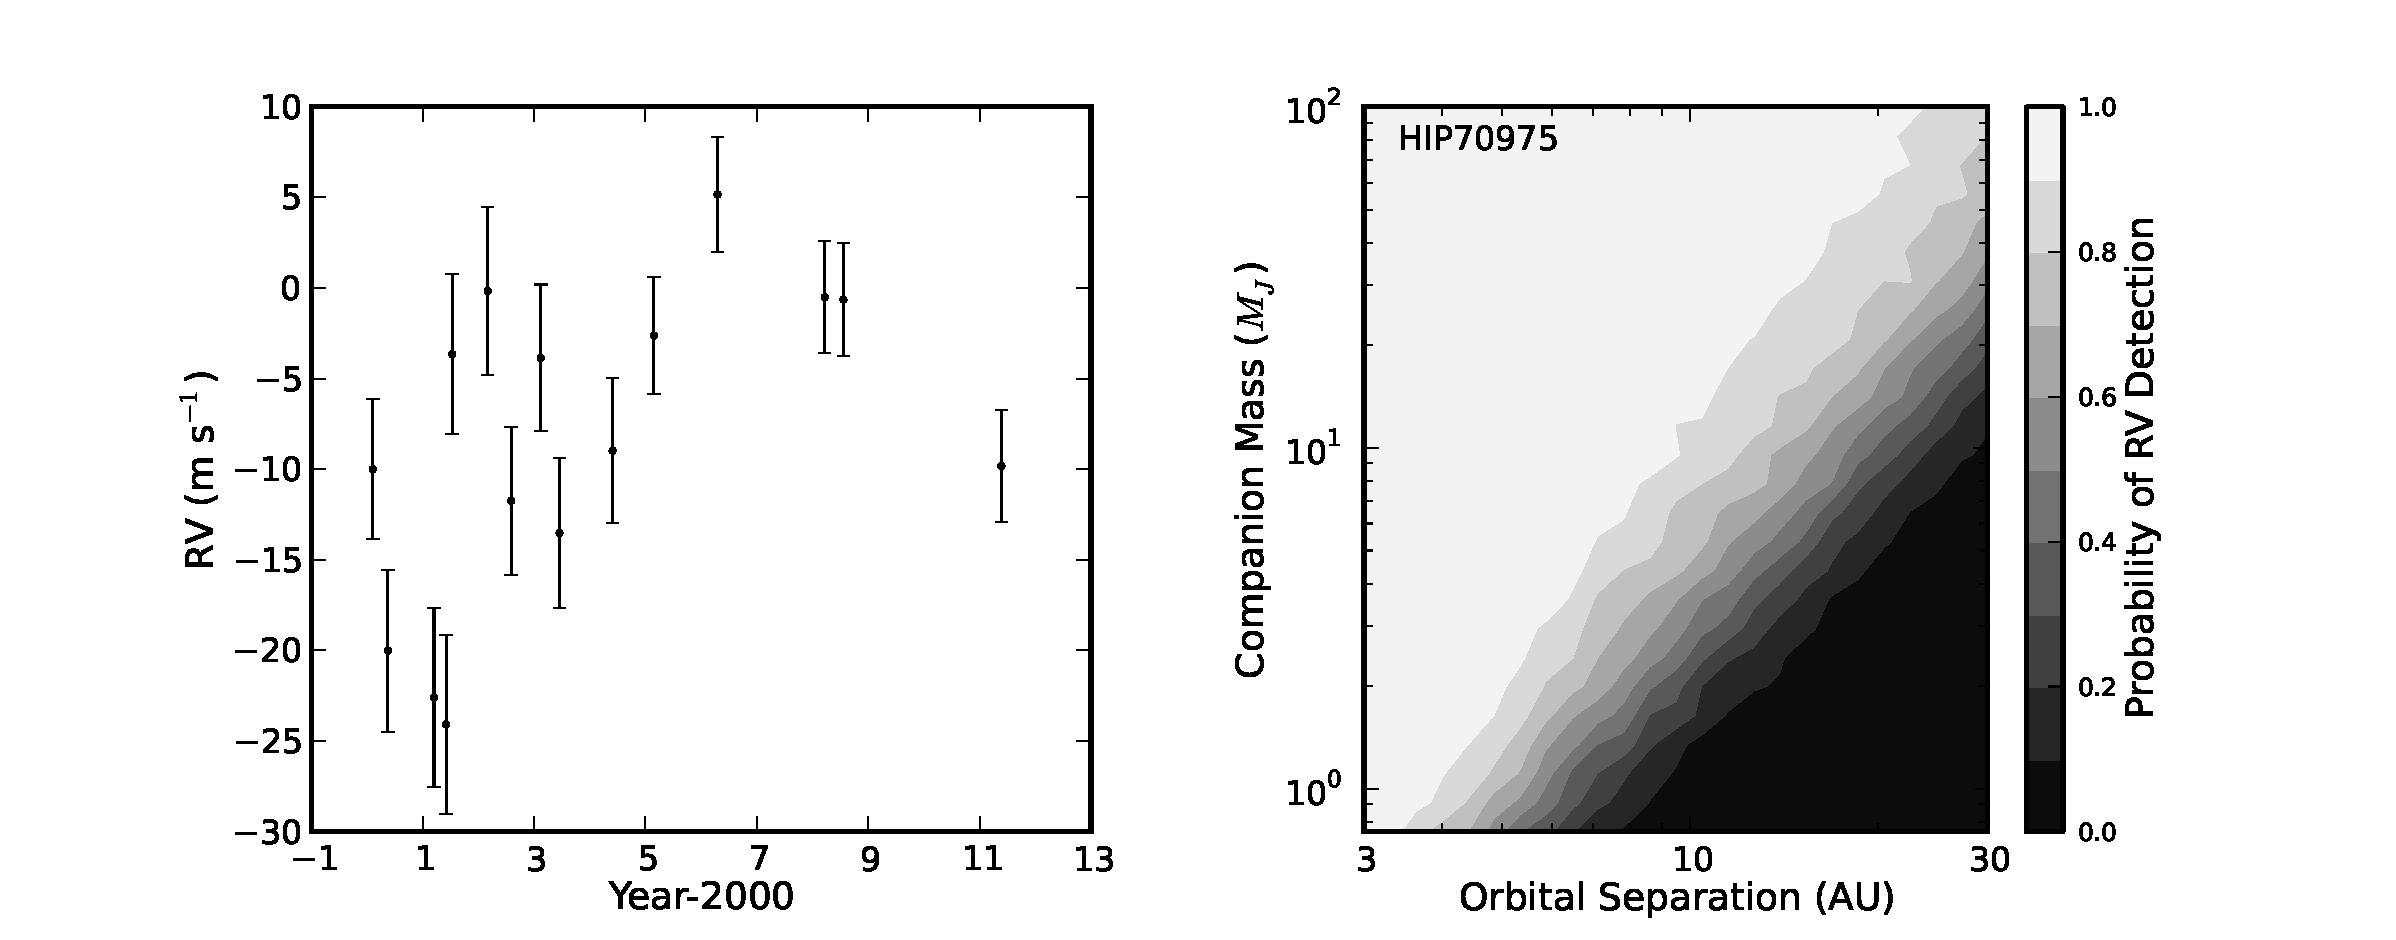
\includegraphics[width=\textwidth]{chapter3/f3.eps}}
\caption[RVs and detectability contours for a typical star in the survey]{(left) RVs for HIP\,70975, a typical star in our survey. This $0.32 M_\odot$ M-dwarf has a total of 15 radial velocity observations over a baseline of 15.5 years, with an average RV precision (including photon noise and jitter) of 4 m/s. (right) Detectability plot showing the likelihood of an RV detection for a companion orbiting HIP\,70975 as a function of companion mass and semimajor axis from its host star. \newline
  }
\label{Detectability}
\end{figure}


\begin{figure}[htbp]
        \centering      
\centerline{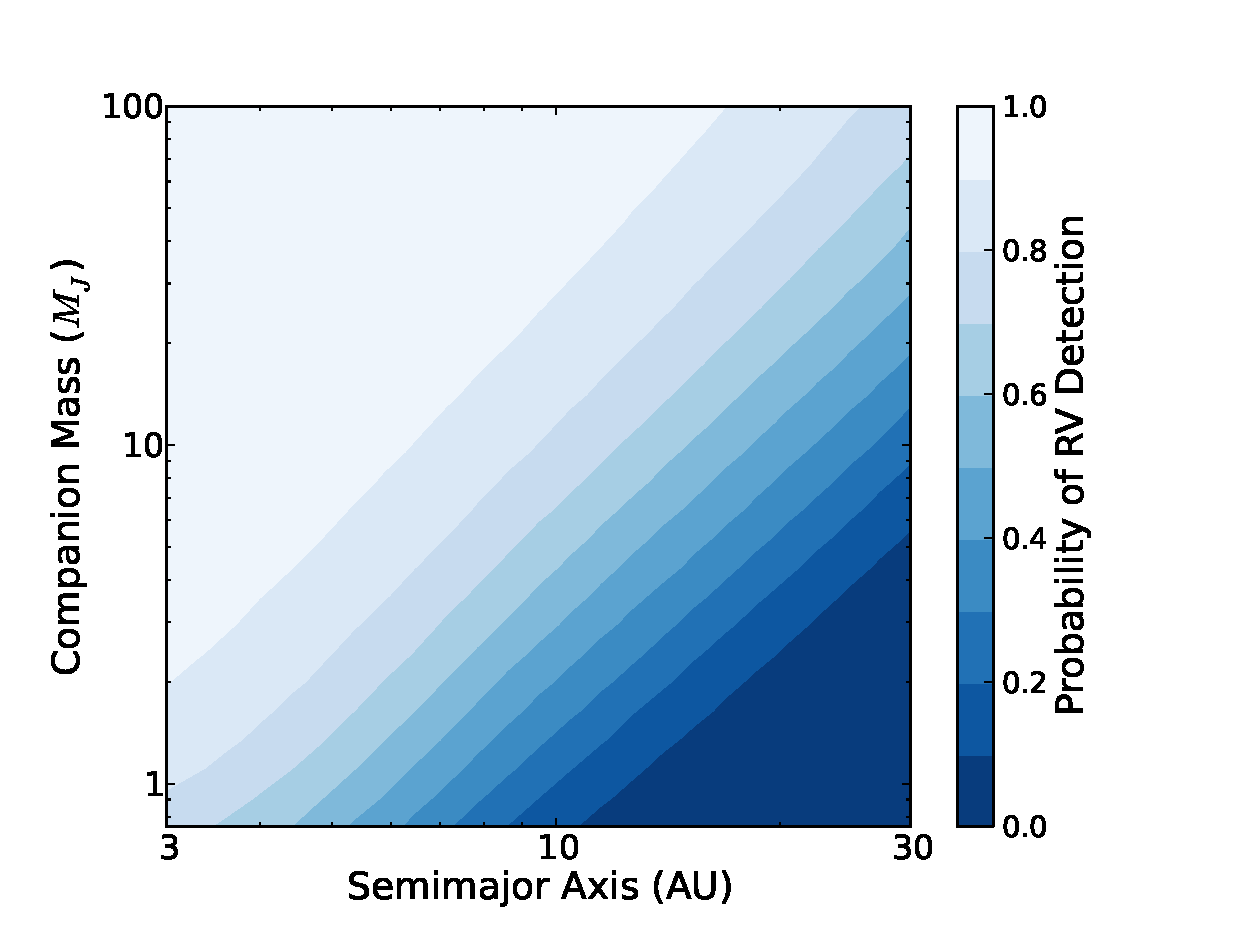
\includegraphics[width=0.75\textwidth]{chapter3/f4.eps}}
\caption[Ensemble likelihood detectability contours for an RV companion,
averaged over all stars in the sample]{The ensemble average likelihood over all 111 stars of an RV detection for a companion to a star in our sample as a function of companion mass and orbital semimajor axis. We can detect accelerations induced by planets as small as $1 M_J$ in short orbits, but a planet distribution function is required to determine the number of $1 M_J$ planets in wide orbits and calculate the overall giant planet occurrence rate.
  }
\label{DetectFull}
\end{figure}

Eight of the stars in our sample host known planets with closed orbits. All of the planets have $m \sin i < 2.5 M_J$ and are listed in Table \ref{knownpl}. To identify radial velocity accelerations caused by outer planets, we include the signal from these planets by comparing a model which contains the known planet and an acceleration to a model which contains only the known planet. Two known planets in our sample, Gl 876b and Gl 317b, are larger than $1 M_J$, so in addition to searching these systems for long-term RV accelerations, we also include these known planets in our giant planet occurrence calculations.
 

One additional planet, Gl\,649b, has a best-fitting mass $m \sin i = 0.90 \pm 0.05 M_J$; if the inclination is smaller than 64 degrees this planet has mass $ m > 1 M_J$. We follow the method of \citet{Ho11} to determine the probability of this event. That is, we define the probability that the true mass $m$ is greater than some value $X$ given an observed mass $m_O = m \sin i$ such that
\begin{equation}
P(m > X | m_O) = 1 - \frac{\int_{m_O}^X \frac{(m_O/m^2)}
{\sqrt{1-(m_O/m)^2}}P(m)dm}{\int_{m_O}^{m_\textrm{max}}
\frac{(m_O/m^2)}{\sqrt{1-(m_O/m)^2}}P(m)dm}
\end{equation}
Here, $P(m)$ is the true planet mass distribution function.
% We apply the distribution found by \citet{Cumming08}, as explained in \textsection{\ref{Methods}}. 
$m_\textrm{max}$ is the physical upper mass limit for a planet. Since the true distribution function is strongly biased towards small planets, the number selected here does not significantly affect our results. By simply assuming the star is aligned randomly along our line of sight so that the inclination distribution is flat in $\cos i$, the result of a flat planet mass distribution function, we expect a observed mass $m \sin i = 0.90 M_J$ to be produced by a Jupiter-mass or larger planet 56\% of the time; all reasonable assumptions of an underlying mass distribution affect this value by less than 10\%. We repeat this procedure for all confirmed planets in our sample with masses $m \sin i < 1 M_J$ to quantify the likelihood that other known planets are $m > 1 M_J$ planets with low inclinations. We find, in addition to Gl\,849b, HIP\,22627b ($m \sin i = 0.64 M_J$) has approximately a 25\% probability of having a mass $m > 1 M_J$. This probability is vanishingly small for all other known planets.

Of our sample of 111 stars, 2 have confirmed planets larger than $1 M_J$, 6 systems have confirmed RV planets with masses $m \sin i < 1 M_J$ only, two exhibit RV acceleration caused by known brown dwarfs, and four show unexplained long-term RV accelerations, such that $\Delta$BIC > 10 when we include an acceleration term in our fit to the RV data. In the case of Gl\,849b, the long-term acceleration exhibits significant curvature, so we are able to place constraints on this object's mass and orbital semimajor axis. In all other cases, the magnitude of the observed acceleration is different from zero by $3\sigma$. Additionally, the magnitude of the acceleration is such that over the observing baseline, the expected $\Delta\textrm{RV}$ induced by the putative outer planet is larger than the uncertanties of each individual data point. The distribution of these systems in the stellar mass-metallicity plane is shown in Figure \ref{massmetal}.

 
\begin{figure}[htbp]
\centerline{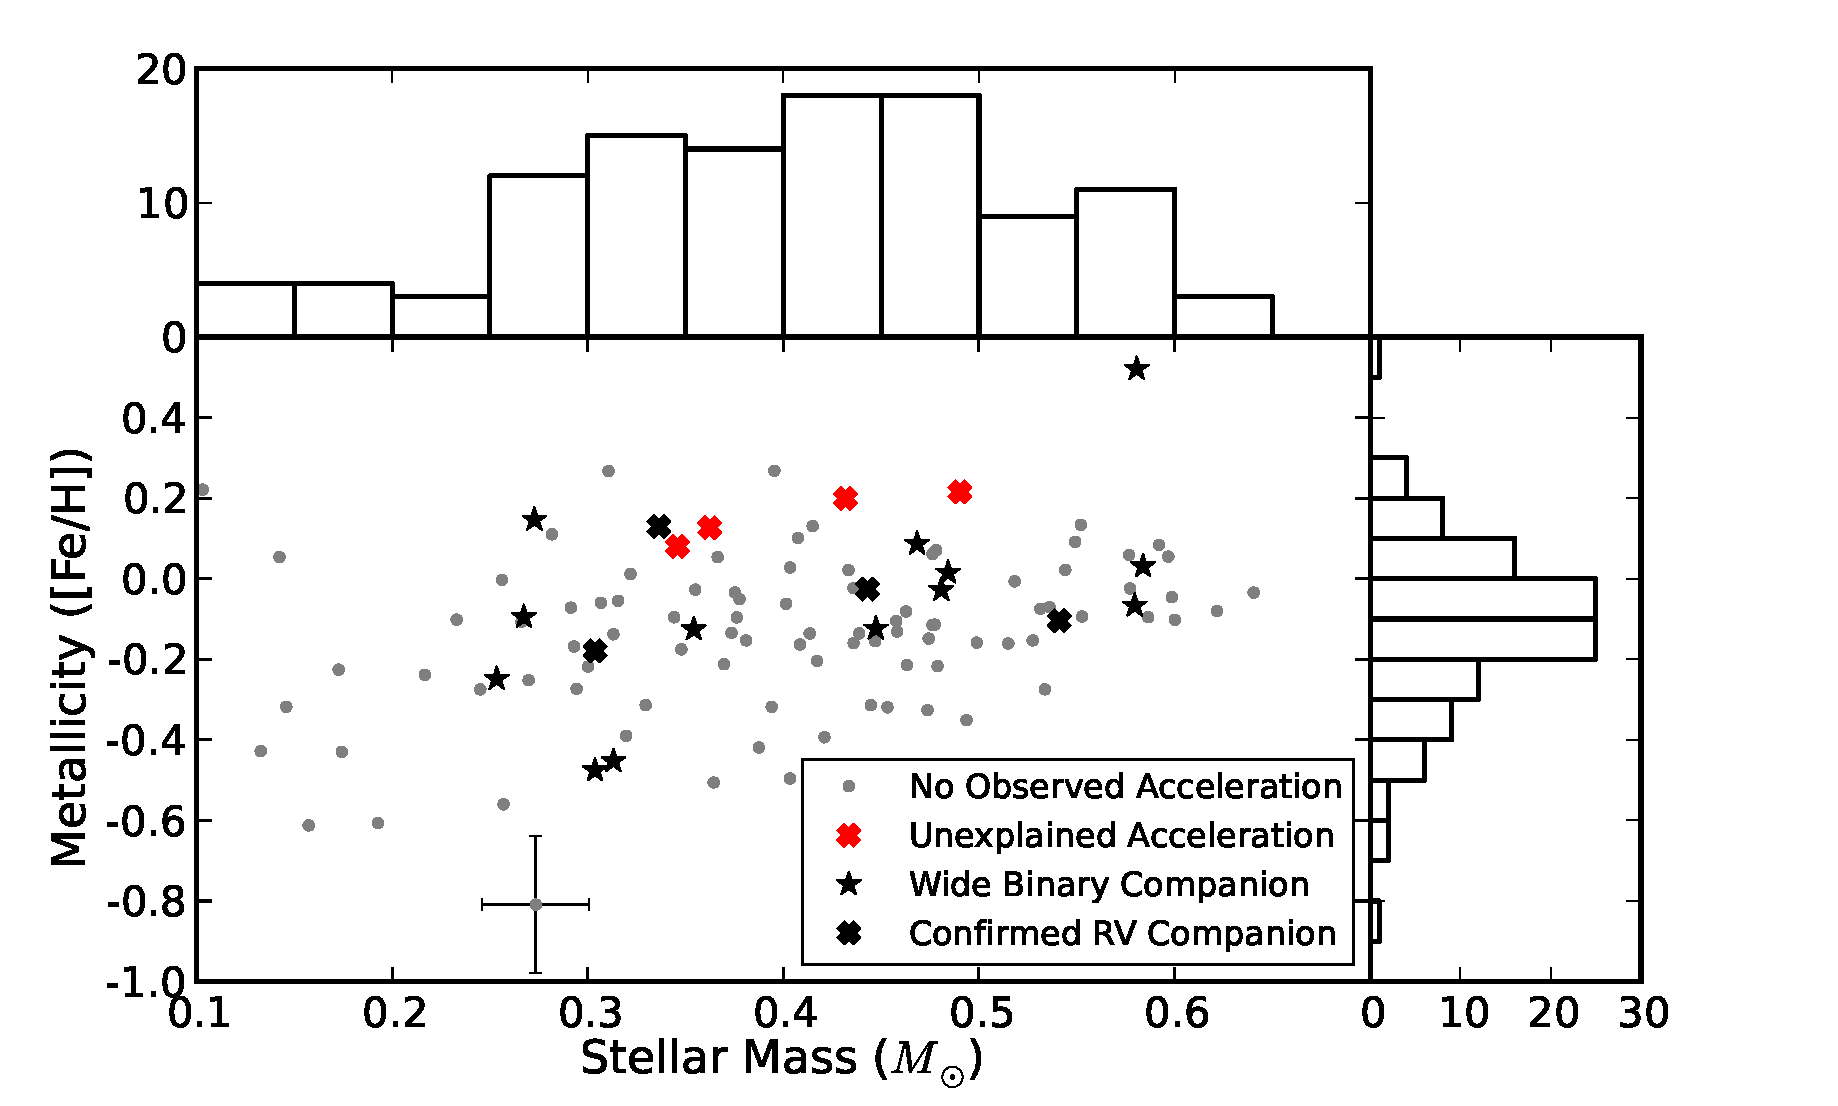
\includegraphics[width=0.95\textwidth,trim={0 0 0 0}, clip=true]{chapter3/f5.eps}}
\caption[Observed M-dwarf sample in the stellar mass-metallicity plane]{Observed M-dwarf sample in the stellar mass-metallicity plane. Systems with observed RV accelerations are shown in red while those without a detected acceleration are in black. Systems with a wide binary companion are labeled with stars, while diamonds represent systems with confirmed planets of any mass. The error bars displayed for HD\,33793 are representative of the uncertainties for all stars in our sample.
  }
\label{massmetal}
\end{figure}


For the four targets with an observable RV drift, we create a grid of logarithmically-spaced companion masses and semimajor axes over the range $0.75 < m/M_J < 100$ and $3 \textrm{AU} < a < 30 \textrm{AU}$. For a given grid point, we determine the best-fitting Keplerian orbit for a given eccentricity and inclination. We assume the inclination and eccentricity distributions are the same as assumed previously. The eccentricity distribution is well-characterized for solar-type stars, but may not hold for planets around lower-mass stars. We find the exact choice of eccentricity distribution does not significantly affect our results.

We determine the likelihood of the best-fitting orbit for each mass, period, eccentricity, and inclination. We then convert these likelihoods into relative probabilities, assuming our errors are uncorrelated so that $P \propto(-\exp(\chi^2/2)))$. We then marginalize over eccentricity and inclination and normalize our probabilities so that $\displaystyle\sum\limits_{M,a} P = 1$. In these cases, we assume the inclination is random on the sky, so that the inclination follows the distribution $f(i) = \sin i$. Assuming a different planet mass distribution function affects this result by less than 10\%. The result is a contour in the mass-semimajor axis plane for the likelihood that a given object could cause the observed stellar radial velocity variation \citep{Wright07}. An example is shown in Figure \ref{WrightRV}. Implicit in this analysis is the assumption the radial velocity variation is dominated by the motion of a single, massive companion rather than the constructive interference of the RV signal of two or more smaller objects. We discuss false positive probabilities in \textsection\ref{FP} and conclude the assumption that one signal dominates the observed RVs is reasonable.

\begin{figure}[htbp]
\centerline{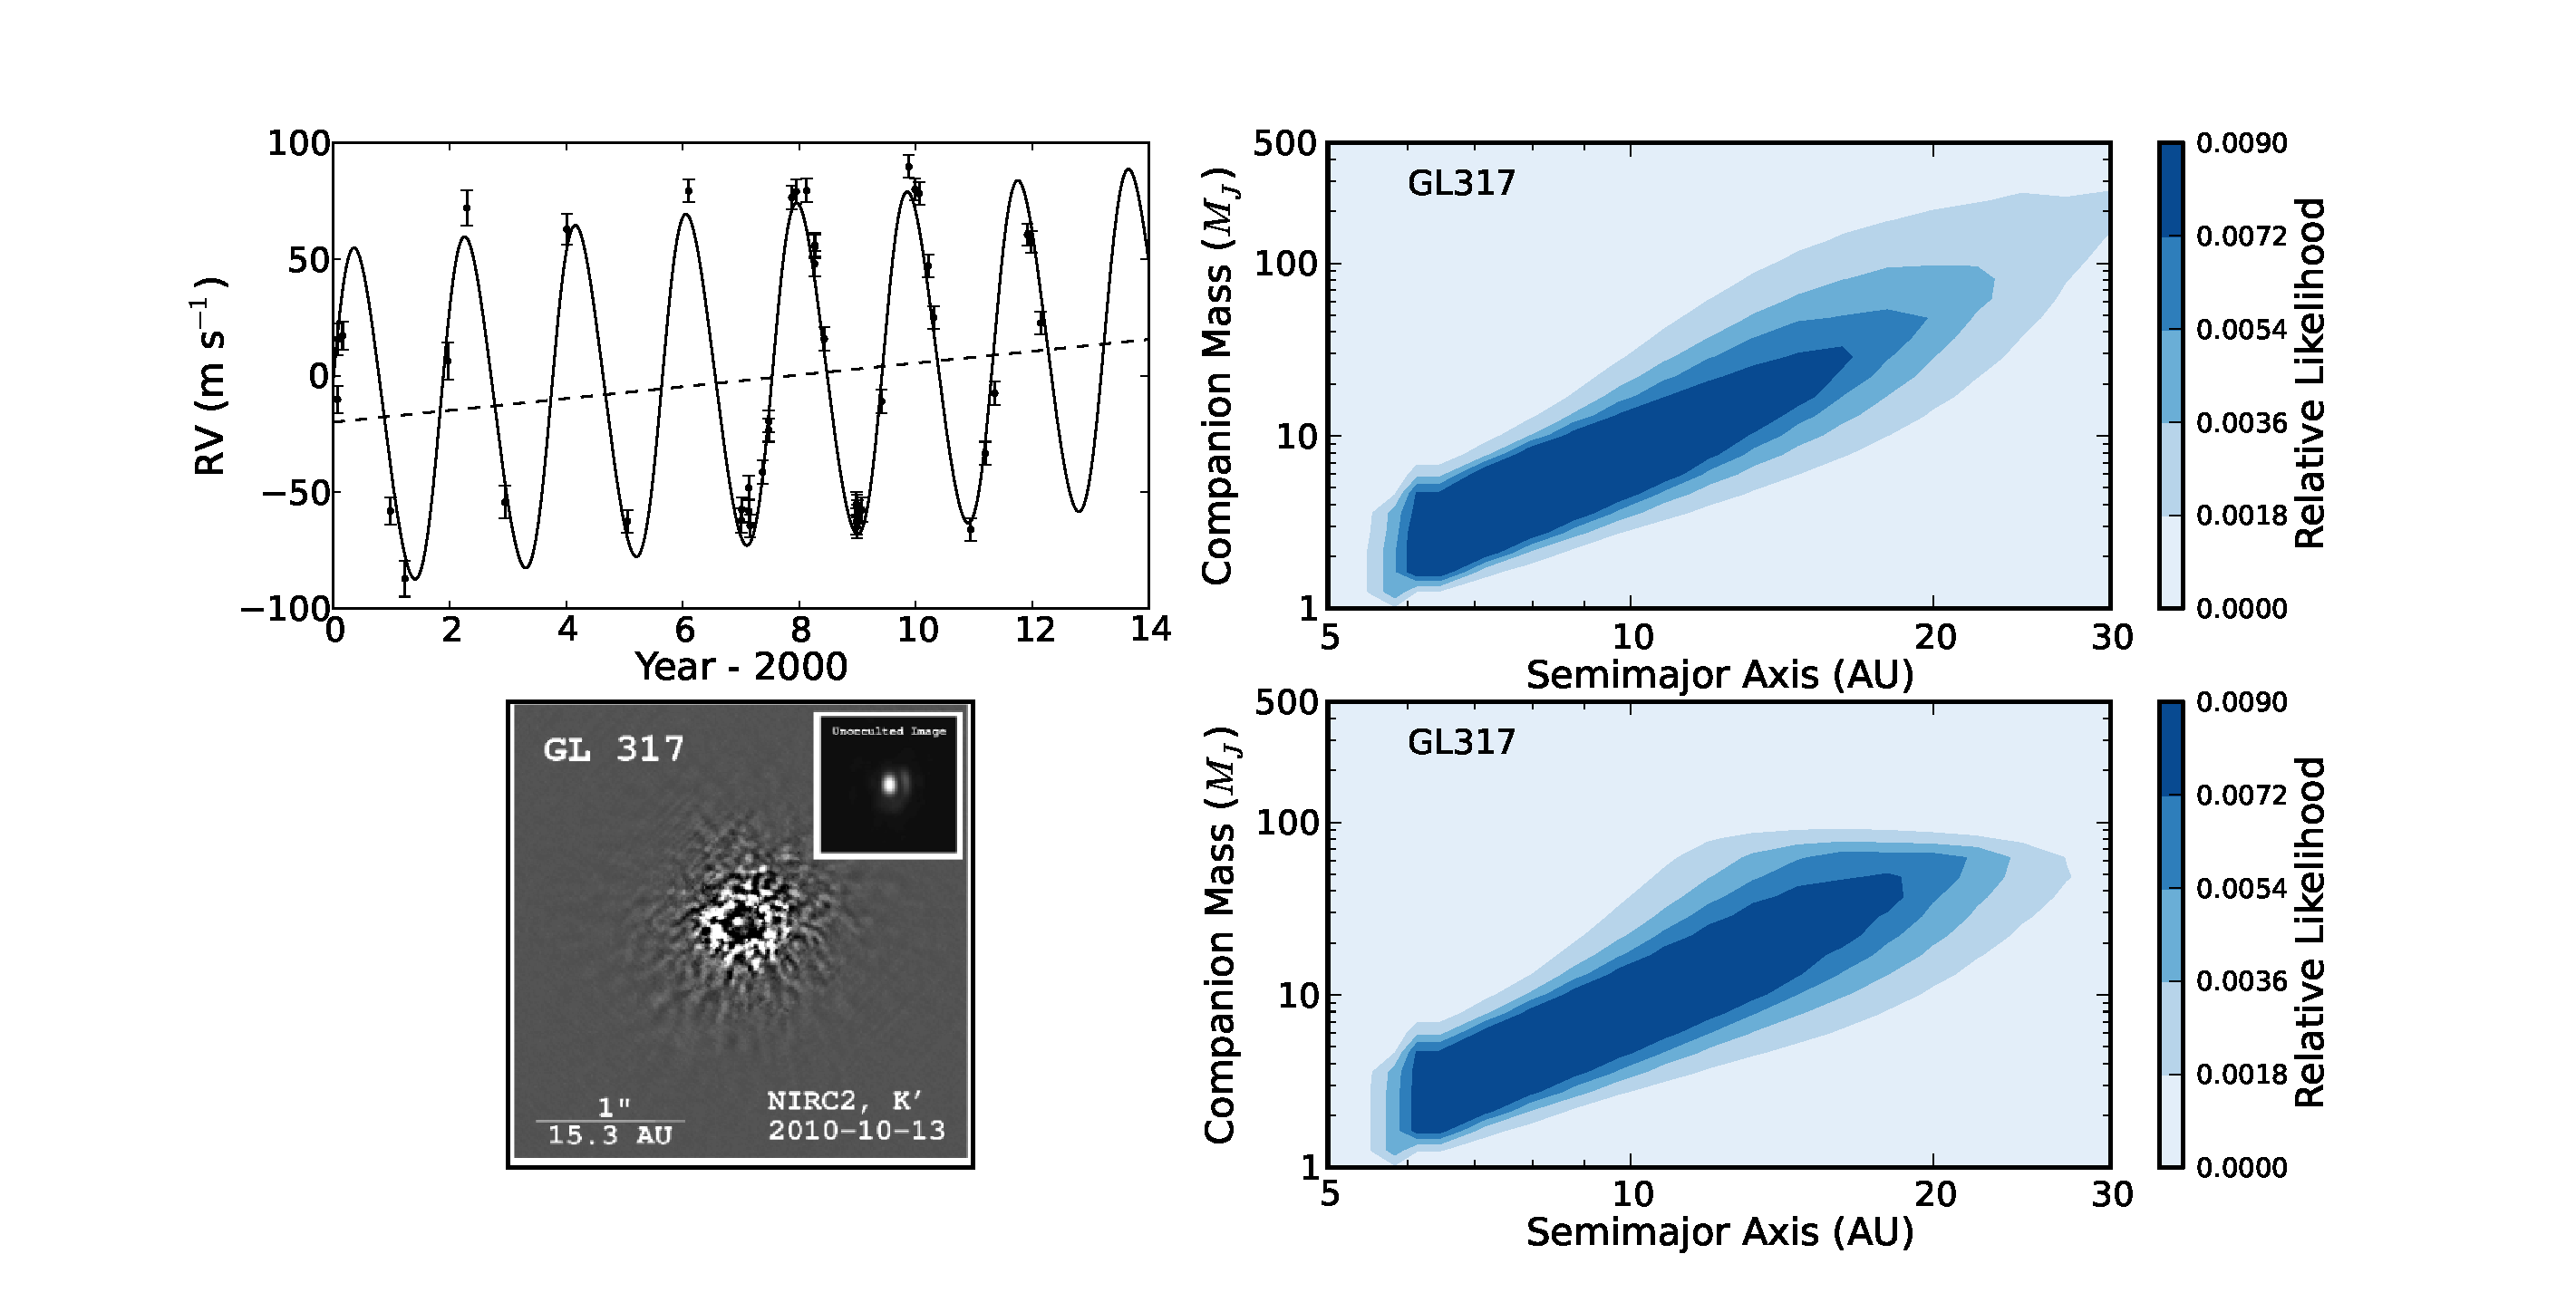
\includegraphics[width=1.0\textwidth, trim={0 0 0 0}, clip=true ]{chapter3/f6.eps}}
\caption[RVs for Gl\,317 and parameter space where a distant companion could reside before and after AO imaging]{(top left) RV observations for Gl\,317 over our 12.1 year baseline. The best-fitting RV acceleration is $-2.51 \pm 0.62$ m s$^{-1}$ yr$^{-1}$ (dashed line); the best-fitting model which includes both the planet and the acceleration is shown as a solid line. (top right) Probability contours marginalized over eccentricity and inclination, displaying the location of a giant companion orbiting Gl\,317 from RVs alone. The likelihood values are normalized such that the sum of the likelihood over our 26x25 grid of companion masses and separations sums to unity. (bottom left) AO image of Gl\,317, showing no companion is visible in the AO imagery, either in the unocculted image (inset) or when a coronagraph is inserted. This eliminates the possibility of a stellar-mass companion at a projected separation smaller than 48 AU. (bottom right) Probability contours displaying the location of a giant companion to Gl\,317 when the RV data is combined with AO data. We find the RV acceleration is likely induced by a substellar companion.
  }
\label{WrightRV}
\end{figure}


The magnitude of an acceleration depends on both the semimajor axis and mass of the companion. For a planet in a circular orbit, the magnitude of the change in radial velocity, $\dot{\gamma} = dv/dt$, is given by
\begin{equation}
\dot{\gamma} = (6.57 \mbox{ m} \: \mbox{s}^{-1} \mbox{yr}^{-1})\bigg(\frac{m_p}{M_J}\bigg)\bigg(\frac{a}{5 \mbox{AU}}\bigg)^{-2} \hat{v}_p \cdot \hat{r}_{los},
\label{TrendSize}
\end{equation}
with $M_J$ the mass of Jupiter and $a$ the orbital semimajor axis. $\hat{v}_p$ and $\hat{r}_{los}$ are unit vectors along the direction of the planet's velocity vector and the line of sight, respectively. When the companion has longitude of periapsis $\varpi = 90$ or $270$, the magnitude of this trend is maximized: $\hat{v}_p \cdot \hat{r}_{los} = \sin i$. To determine if our observed accelerations are caused by planets or more massive companions, we obtained AO imaging observations of each star.




\subsection{Adaptive Optics Observations}
\label{AO Description}
The detectability diagnostics developed in \textsection\ref{RVs} are based strictly on the information encoded in the RV data. Since we are looking at accelerations caused by objects in wide orbits around the primary star, we must break the degeneracy between companion mass and orbital semimajor axis for a given observed acceleration. AO imaging allows us to immediately detect the presence or nonexistence of nearly all stellar-mass companions and most brown dwarf companions to our primary stars, so we can readily separate stellar-induced accelerations from those caused by planets. 

All four targets with an observable RV acceleration were observed with NIRC2 (instrument PI: Keith Matthews) at the W.M. Keck Observatory using the AO system \citep{Wizinowich00} (Table \ref{T2}). In most cases, images were obtained in the $K^\prime$ filter ($\lambda_c = 2.12 \mu$m). We nominally execute a three-point dither pattern to facilitate removal of instrument and sky background noise. Images were processed by flat-fielding, correcting for hot pixels with interpolation, subtracting the sky background, and rotating the frames to standard north-east orientation. In three cases, we applied the angular differential imaging (ADI) point spread function subtraction technique, allowing the observed field to rotate around the target star during the observation, while instrumental artifacts remain fixed. In all cases, we use the large hexagonal pupil mask and the narrow camera. For all four systems exhibiting long-term RV accelerations, we did not image a massive companion. In the cases where our field of view is not large enough to eliminate the possibility of massive stars in very wide orbits ($ > 4''$), we supplement our AO data with publicly available 2MASS images. 
 

The luminosity ratio between our M-dwarfs and their companions depends on the mass of the companion and the age of the system. Stars observed by the CPS team are selected to avoid excessive chromospheric activity, and are thus likely older than 1 Gyr \citep{Wright05}. We assume all targets have fully contracted and assert an age of 5 Gyr for each system. For systems with nondetections, we estimate the flux (and thus the mass) a companion would need to have to be observed at a given projected separation in our observations. From that value, we can then determine the region of parameter space excluded by the observations (Figure \ref{CCplot}). In general, AO imaging eliminates nearly all stellar companions, while ADI can also probe the brown dwarf mass regime.

For each of our targets with unexplained accelerations, a contrast curve showing the mass to which we are sensitive to companions at the $5\sigma$ level as a function of projected separation is shown in Figure \ref{CCplot}. This choice provides similar results to the detection limits found by visual inspection, as tested by injecting artificial companions into AO images \citep{Metchev09}. We convert relative brightness to mass using the theoretical evolutionary tracks of \citet{Baraffe03} for substellar companions and \citet{Girardi02} for more massive companions. Interpolation between the two sets of models provides reasonable results in the intermediate domain near $125 M_J$. The resultant parameter space where a companion could reside to cause the observed stellar acceleration is shown in Figure \ref{WrightRV}. 



\begin{figure}[htbp]
\centerline{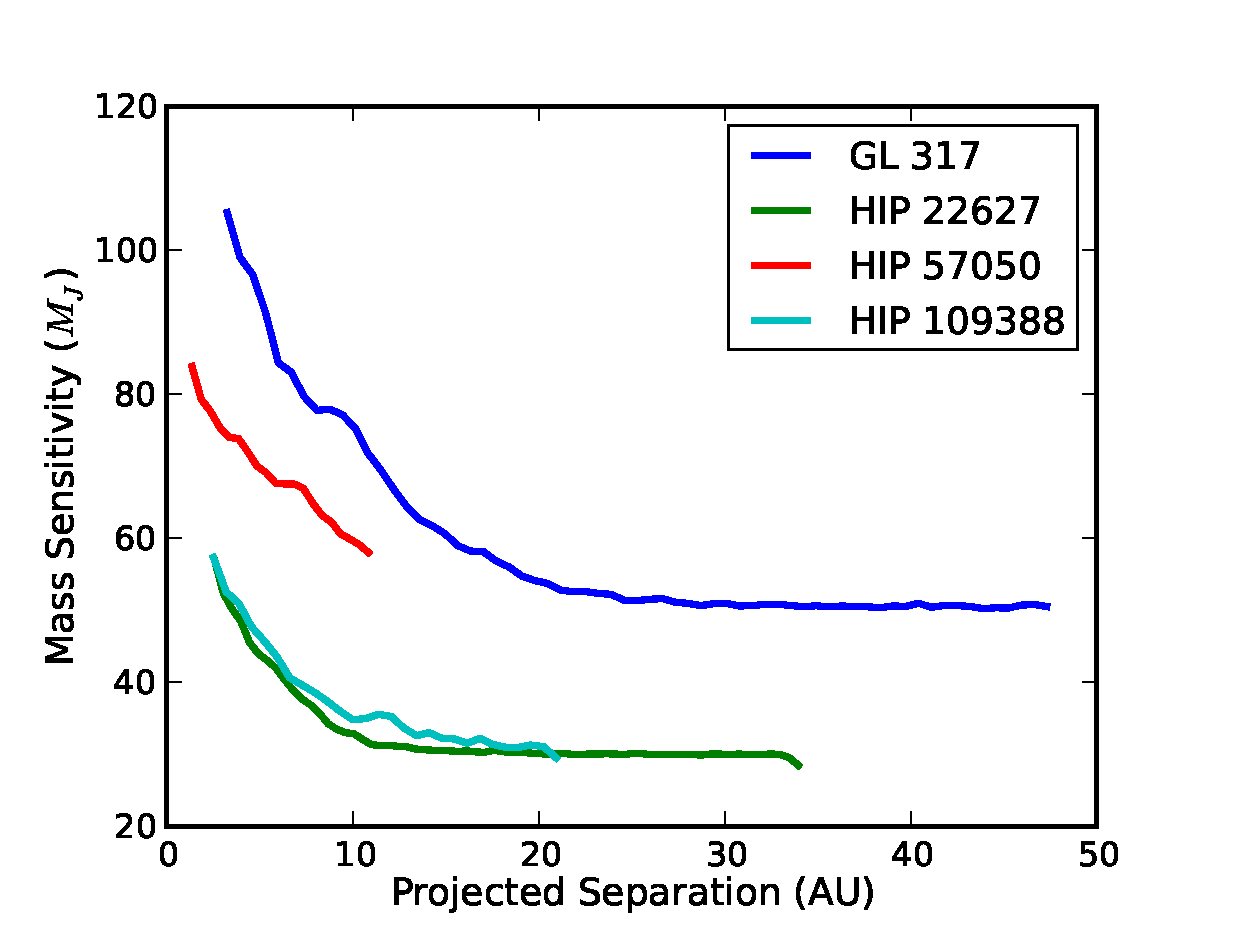
\includegraphics[width=0.75\textwidth]{chapter3/f7.eps}}
\caption[Mass sensitivity for a $5\sigma$ AO detection of a companion
as a function of projected angular separation]{Mass sensitivity for a $5\sigma$ detection of a companion object as a function of projected angular separation for each of our four stars with long-term RV drifts. The maximum projected separation eliminated corresponds to the field of view of the AO system and thus varies for each star as a function of the distance to each star. For all stars except HIP\,57050, we rule out stellar mass companions beyond 1 arcsecond through our adaptive optics imaging. When our field of view is small, we supplement our AO data with 2MASS seeing-limited images. Stellar companions at small projected separations would have RV accelerations larger than those observed in our sample. 
  }
\label{CCplot}
\end{figure}

The assumption of a 5 Gyr age for each star does not significantly affect our results. For all plausible system ages, stellar mass companions would be easily detectable by AO. Our sensitivity to stars is independent of assumed age, as luminosities of M-dwarfs are constant over the age of the universe. At no ages $> 1$ Gyr are we sensitive to any planetary mass companions. As shown in Figure \ref{AgeAO}, assuming a different age for each star would only change the efficiency of detecting brown dwarfs. Since the occurrence rate of brown dwarfs is only a few percent, much smaller than the occurrence rate of planets or low-mass stars \citep{Metchev09, Dieterich12}, errors induced by assuming an incorrect stellar age from missed brown dwarfs are small. ``False negatives'' such as these will be discussed in \textsection\ref{FN}.

\begin{figure}[htbp]
\centerline{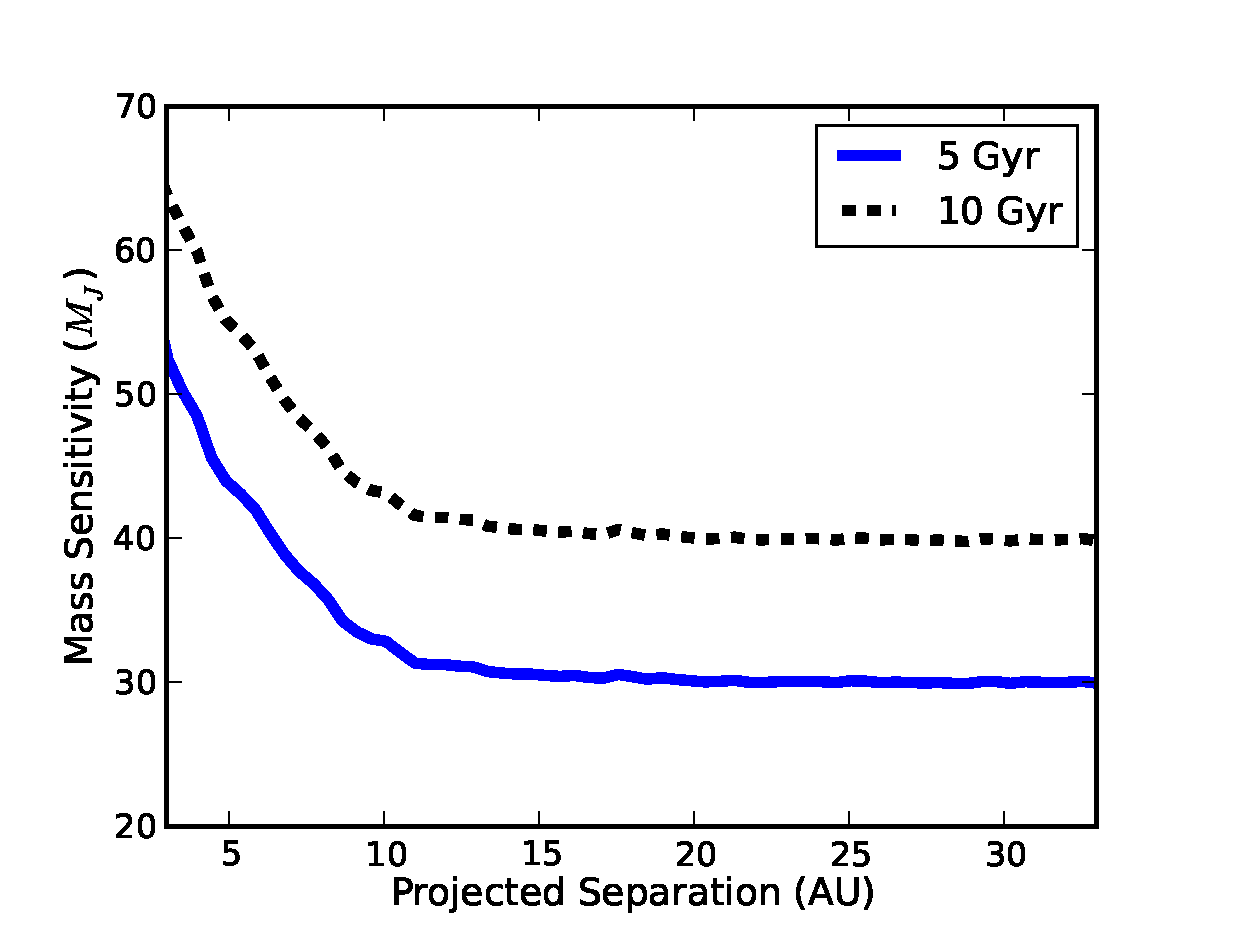
\includegraphics[width=0.75\textwidth]{chapter3/f8.eps}}
\caption[Mass exclusion plot for HIP\,22627 showing the insensitivity of our results to assumed stellar age]{Adaptive optics mass exclusion plot for the star HIP\,22627 showing the relative insensitivity of our results to the assumed age of M-star planet hosts. Adaptive optics observations rule out essentially all stellar mass companions. Sensitivity to substellar objects is a function of age, but brown dwarfs are scarce at close separations \citep{Marcy00}, and wide separations \citep{Metchev09}. Thus, our estimate of the planet frequency around M-stars is only weakly dependent on our assumed age of the host stars.  
  }
\label{AgeAO}
\end{figure}



\section{Measuring the Giant Planet Occurrence Rate}
\label{Stats}

We estimate the occurrence rate of giant planets orbiting M-dwarfs using statistical inference. The fraction of stars which host giant planets, given some number of observed accelerations $N\scriptsize{\mbox{trends}}$ and some number of nondetections $N\scriptsize{\mbox{ND}}$ from a sample of targets, is given such that
\begin{equation}f_{pl} = \frac{N\scriptsize{\mbox{trends}}\normalsize P(\mbox{planet}|\mbox{trend}) + N\scriptsize{\mbox{ND}}\normalsize P(\mbox{planet}|\mbox{ND})}{N\scriptsize{\mbox{targets}}}
\label{ResultEq}
\end{equation}
To calculate the posterior probability that a given star hosts a gas giant planet, we must estimate the \textit{a priori} likelihood that a planet exists given the presence of an RV acceleration (a true positive), the likelihood a planet would not be detected in an RV survey (a false negative) and the likelihood that an observed acceleration is caused by some effect other than the movement of a planet (a false positive). 

\subsection{False Negatives}
\label{FN}

There are multiple ways for a giant planet to be missed in our survey. For each planet in a wide orbit, we observe only a fraction of a revolution. A planet near its maximal sky-projected separation from its host star has acceleration primarily in the tangential, not radial, direction. In cases such as this the change in radial velocity over our observing baseline may not be noticeable. Thus we may expect to have a lower RV detection efficiency for planets near their maximal sky-projected separation. 

Similarly, we may expect to have a lower imaging detection efficiency for stars near their minimal sky-projected separation, when the RV acceleration is the largest. However, in these cases we would still expect to detect the binary companion. If the companion is located directly along the line of sight to the star, then it will also appear in the 0''.85 spectrograph slit used with HIRES. Therefore, we would expect such systems to appear as SB2s. We explore this fully, and show that we would detect all such systems, in \textsection\ref{PMBS}.

To determine the likelihood that such a planet would be missed by our search, we use our detectability matrices developed in \textsection\ref{RVs}. We assume the distribution of planets follows a double power-law, such that
\begin{equation}
\frac{d^2N}{d\log m d\log a} \propto m^{\alpha} a^{\beta},
\label{DPL}
\end{equation}
similar to that assumed by \citet{Cumming08} and \citet{Bowler10}, and comparable to the power-law distributions applied in the analyses of microlensing surveys. At a given companion mass and semimajor axis, we can then determine the relative likelihood that a planet exists at this position. We multiply this by the likelihood of detecting such a planet to determine the fraction of planets we would find orbiting each star and the fraction we would miss. These numbers are determined through our analysis of observations of simulated injected planets, as developed in \textsection \ref{TS}.

We can test our detectability calculation by analyzing the known wide-separation companions in our sample. Of our 111 stars, four are known to host directly imaged brown dwarf companions. Of these, two (HD\,71898B and HIP\,63510B) were detected as accelerations in our sample, while two (Gl\,569B and Gl\,229B) are at very large separations and were not detected. The detection or nondetection of each system is consistent with what would be expected from our analysis of injected planets.



We detect the two brown dwarfs with high expected RV detection efficiency, and do not detect the two with expected detection efficiencies near zero, both of which have $a > 40$ AU. We would like a larger sample to test this method, but the limited number of brown dwarfs suggests our ability to detect giant planets is consistent with expectations. This sample also suggests $f_{BD}$ is only a few percent, consistent with complementary studies \citep{Dieterich12}.


A giant planet could also be missed if it was in a system with multiple giant planets. We observe only the sum of all radial velocity signals from all planets orbiting a star. For example, if a star hosts two giant long-period planets with one on each side of the star, the two signals would destructively interfere. Even if the acceleration was still detectable, this interference would cause us to measure an incorrect magnitude of the acceleration, so our probability contours would be incorrect. Giant planet multiplicity around M-dwarfs is not well understood, but since giant planet occurrence is believed to be small \citep{Bonfils13} the multiplicity rate of giant planets around M-dwarfs is likely also small. Presently, there are no known systems with two planets larger than Jupiter orbiting one M-dwarf. Even in cases with two large planets, one planet will dominate the RV signal. For example, OGLE-2006-BLG-109L contains a $0.73 \pm 0.06 M_J$ planet at $2.3 \pm 0.5$ AU and a $0.27 \pm 0.02 M_J$ planet (slightly less massive than Saturn) at $4.5^{+2.1}_{-1.0}$ AU \citep{Gaudi08, Bennett10}. In this case the Doppler amplitude of the inner planet would be a factor of 3.3 larger than the Doppler amplitude of the outer planet. Similarly, an external observer of the solar system would observe an RV signal from Jupiter 4.5 times larger than that of Saturn. Thus we neglect this possible source of error.


We then claim that the likelihood of the existence of a giant planet given the nondetection of an RV acceleration is 
\begin{equation}
P(\mbox{planet}|\mbox{ND}) = f_{pl}(1-\eta_{pl,\star})
\label{FNP} 
\end{equation}
where $\eta_{pl, \star}$ is the probability of detecting a giant planet around a given star as a function of planet mass and orbital semimajor axis, estimated by simulating observations of injected planets. The true probability of missing a planet depends on the true giant planet occurrence rate and the planet distribution function. We can determine this value directly if the underlying planet distribution function (Equation \ref{DPL}) is assumed. By counting the observed trends and analyzing our RV detection efficiencies for each star as a function of mass and separation, we can determine the number of missed planets. We find our final result is not a strong function of mass index $\alpha$ or semimajor axis index $\beta$ (see \textsection\ref{PL}).

\subsection{False Positives}
\label{FP}
\subsubsection{Multiple Planets}
In some cases, observed accelerations may not be induced by the orbit of a giant planet. If two smaller planets are orbiting one star, when they are both on the same side of the star their RV signals would constructively interfere, giving the appearance of a giant planet where none exists. Again, multiplicity rates of large planets are unknown for these small stars but are likely small; we again neglect this effect as a possible source of error. This is a reasonable assumption even if the multiplicity rate of gas giant planets around M-dwarfs was much larger than currently expected. Both the orientation of the system and the relative positioning of the planets during our observations is random. Therefore, it is equally likely that multiple planets would be in the ``constructive'' or ``destructive'' phase of their orbits. Thus, similar numbers of false additional planets would be added to our sample as missed true planets. 

\subsubsection{Secular Acceleration}
A false positive can also be caused by secular acceleration. When a high proper motion star moves quickly relative to the Sun, its peculiar velocity vector changes direction in time, causing the star's systemic radial velocity to increase. For a star with proper motion $\mu$ at a distance $d$ the magnitude of this effect is, to first order,
\begin{equation}
\dot\gamma = 23.0 \textrm{ cm s}^{-1} \textrm{ yr}^{-1} \bigg(\frac{d}{10\textrm{ pc}}\bigg)\bigg(\frac{\mu}{1 \textrm{ arcsec yr}^{-1}}\bigg)^2.
\end{equation}
The secular acceleration $\dot\gamma$ is always positive, so that the star's radial velocity only increases because of this effect. For several nearby stars secular acceleration is large enough to create an apparent acceleration or cause an astrophysical RV acceleration to be incorrectly measured. For example, Barnard's star has a secular acceleration of $4.515 \pm 0.002$ m s$^{-1}$ yr$^{-1}$ \citep{Choi13}, larger than all of our observed accelerations. Fortunately, the magnitude of the secular acceleration can be precisely quantified if the star's distance and proper motion are known. All of our stars have measured proper motions and parallaxes, so we can determine the expected secular contribution. This acceleration is subtracted from the observed radial velocity automatically by the CPS RV pipeline \citep{Howard10}, so this potential source of error is automatically accounted for in our data. Moreover, none of our observed accelerations are consistent with what would be expected from secular acceleration alone. 

\subsubsection{Magnetic Activity}
\label{MA}
Magnetic activity on a star can cause a false positive: rotating active regions can affect the shape of the observed spectral lines and thus the apparent RV \citep{Gray88}. A magnetic cycle can occur over years and hide or mimic a radial velocity signal. We denote the fraction of stars with a magnetically-induced acceleration as $f_A$. \citet{GomesdaSilva12} claim six stars from their sample of 27 M-dwarfs with variability ($22\% \pm 9\%$) have RVs induced by magnetic activity. We are interested in the converse (how many trends are induced by variability?) but their result suggests $f_A$ may be significant. To determine $f_A$, we review all 165 M-dwarfs observed by the CPS team, both as part of this survey and as part of the M2K survey \citep{Apps10, Fischer12}. Between these two programs, there are a total of 34 systems with RV trends. We analyze the $S_{HK}$ values for these stars and find the RV correlates with $S_{HK}$ with a correlation coefficient $|r| > 0.5$ in 7 cases, suggesting $20.6\% \pm 7.8\%$ of long-term RV trends may be magnetically induced. We adopt this value as $f_A$. Even if the true value for $f_A$ is a factor of two larger, it would decrease our planet occurrence rate from $f_{pl} = 6.5\%$ to only $f_{pl} = 4.9\%$, still within our uncertainties.

\subsubsection{Brown Dwarfs}
\label{BD}
Our adaptive optics search is sensitive to all stellar-mass companions, but only to the most massive brown dwarfs. We can detect brown dwarfs larger than approximately $50 M_J$, although this number varies from target to target. For each target, we can determine the fraction of brown dwarfs we would expect to detect by our adaptive optics imaging, given the assumption that a trend was caused by a brown dwarf. We call this efficiency $\eta_{BD}$. Here, we assume a form for the brown dwarf mass function where $dn/d\log(m) \propto m^{0.4 \pm 0.2}$ \citep{Pena-Ramirez12}. Thus we can estimate the likelihood of detecting a brown dwarf around a star in our sample, given that a brown dwarf exists. To estimate the probability a brown dwarf exists, we use the result of \citet{Dieterich12}, who, through an HST/NICMOS snapshot program, estimate that $f_{BD} = 2.3^{+5.0}_{-0.7}\%$ (at $1\sigma$) of M-dwarfs have an L or T companion between 10 and 70 AU. This is consistent with the result of \citet{Metchev09}, who estimate a brown dwarf companion frequency of $f_{BD} = 3.2^{+3.1}_{-2.7}\%$ (at $2\sigma$) around solar-type (FGK) stars.

\subsubsection{White Dwarfs}
\label{WD}
Compact stellar remnants are often faint and such binary companions can evade direct detection, especially when the compact object is cool ($T < 4000 K$) so that the infrared light is dominated by the primary star \citep{Crepp13b}. Since our targets are all M-dwarfs, it is not unreasonable to expect that some may have formed as lower mass companions in binary systems with the higher mass object having evolved off the main sequence to become a white dwarf.  \citet{Napiwotzki09} combine observations of local white dwarfs with galactic structure models and find that in the thin disk there is a white dwarf number density of $n_{WD} = 2.9 \times 10^{-3}$ pc$^{-3}$. From an analysis of PanSTAARS data, \citet{Wheeler12} estimate 20\% of all white dwarfs have an M-dwarf companion ($f_{M|WD}$), somewhat larger than the 12\% found by \citet{Napiwotzki09}. Considering the measurement by \citet{Chang11} of $n_\star = 0.030 \pm 0.002$ stars per cubic parsec, and that approximately 70\% of all stars are M-dwarfs \citep[$f_{M|\star}$,][]{Henry06}, we can determine the fraction of M-dwarfs in the thin disk with a white dwarf companion, a number we define as $f_{WD}$. If we take $f_{M|WD} = 0.16 \pm 0.04$, we find that 
\begin{equation}
f_{WD} = \frac{n_{WD}f_{M|WD}}{n_\star f_{M|\star}} = 2.2\% \pm 0.5\%,
\end{equation}
where the error is dominated by the uncertainty in $f_{M|WD}$.

By combining the false positive events from \textsection\ref{MA}, \textsection\ref{BD}, and \textsection\ref{WD}, we conclude that given the existence of a trend in our data, the likelihood it is caused by a giant planet is 
\begin{equation}
P(\mbox{planet}|\mbox{trend}) = (1-f_A)[1-f_{BD}(1-\eta_{BD, \star})](1-f_{WD})
\label{FPP}
\end{equation}

\subsection{Determining $f_{pl}$}
\label{Methods}

We determine the giant planet occurrence rate, $f_{pl}$ by combining our estimate of the number of false positives and false negatives with the number of observed accelerations. Specifically, the occurrence of giant planets is given by Eq. \ref{ResultEq} if the number of observed accelerations is known, along with the probability of a false negative or false positive in our sample. These probabilities are defined by Equations \ref{FNP} and \ref{FPP}, respectively. 

For each star in our sample, we use our map of giant companion detectability (e.g. Figure \ref{WrightRV}) to estimate our efficiencies, $\eta_{BD}$ and $\eta_{pl}$. We measure the total planet fraction, $f_{pl}$ and its uncertainty through a Monte Carlo experiment. For each trial, we establish an expected number of observed accelerations, drawing from a binomial distribution with $n=111$ and $p = 4/111$, representing the most likely underlying distribution behind our observed sample. In practice, we draw from our star list 111 times, with replacement, to determine a stellar sample. We then draw randomly from our previously defined distributions to estimate $f_A$, $f_{BD}$ and $f_{WD}$. These values are sufficient to calculate the probability an observed acceleration is caused by a false positive astrophysical event. In cases where known planets with masses $m > 1 M_J$ exist in our sample, we include their presence in our calculation of $f_{pl}$. 

The derivative of the RV acceleration (the ``jerk'') for Gl\,849 is nonzero, so we can use the RV information to fit a two-planet model to this system, instead of a planet plus a linear acceleration. We find the inner planet to have a mass $m\sin i = 0.90 \pm 0.05 M_J$ with a period of $5.24 \pm 0.07$ years, and the outer planet to have a mass $m \sin i = 0.70 \pm 0.31 M_J$ with a period of $19.3^{+17.1}_{-5.9}$ years. More data is needed to determine the exact parameters of the orbit of Gl\,849c, but from the existing RV information we can determine the probability each planet has a mass $m > 1 M_J$. The exact value depends on the planet mass distribution function; assuming each orientation has equal probability (so that $\alpha=-1$) we find probabilities of 0.577 and 0.419, respectively. Following the method of \citet{Ho11}, we find changing the distribution function changes these values by less than 10\%. 

% Make sure there's nothing here for @OverheardOnAph to pick up

Since we know the region of mass-separation parameter space to which we are sensitive to planets for each star, we can self consistently estimate the planet frequency in this parameter space. We then assume the result from \citet{Cumming08}, who find the power-law indices (Eq. \ref{DPL}) of $\alpha = -0.31 \pm 0.20$ and $\beta = 0.39 \pm 0.15$. We randomly select values for $\alpha$ and $\beta$ from these distributions and use our detection efficiencies to determine the number of false negative missed planets in our sample. Through Equation \ref{ResultEq}, we then have enough information to estimate the planet fraction as a function of each parameter. By repeating this process many times, varying each of our assumed parameters, we can measure the overall planet fraction and its uncertainty.


\section{Results and Discussion}
\label{Results}
\subsection{The Frequency of Giant Planets}
\label{R1}

Given an observed trend, we can estimate the likelihood the signal is caused by a massive planet. By analyzing our 111 targets as described in \textsection\ref{Methods}, we recover a distribution in giant planet occurrence as shown in Figure \ref{HistoResult}. We find from this analysis that $6.5\% \pm 3.0\%$ of all M-dwarfs host a giant planet with a semimajor axis smaller than 20 AU. This number is lower than previous studies of higher-mass stars. \citet{Bowler10} find $24^{+8}_{-7}\%$ of ``retired'' A stars host Jupiter-mass planets within 3 AU, while \citet{Cumming08} find that $f_{pl} = 10\% \pm 1\%$ of FGK stars host Jupiter-mass planets within 20 AU. 

If we consider multiplicity in situations where we have a giant planet and an RV acceleration (or in the case of Gl\,849, two giant planets), then we measure a giant planet occurrence rate of $0.083 \pm 0.019$ giant planets per star. To estimate this, we repeat the calcuations of the previous section, but count known giant planets separate from observed accelerations in the cases when we observe both a planet and a ``trend.'' This number does implicitly assume that observed accelerations are caused by the motion of one giant planet, not a combination of multiple planets in motion. The multiplicity rate of giant planets around M-dwarfs appears to be lower than the multiplicity rate of small planets, such as those detected by \textit{Kepler} \citep{Youdin11}.

Our result is consistent with the result of microlensing surveys of M-dwarfs, which suggest a total occurrence rate of $0.09^{+0.03}_{-0.05}$ giant planets per star in the range $1 M_J < m < 10 M_J$ and $0.5$ AU $< a < $20 AU \citet{Cassan12}. However, the power-law distribution determined by the microlensing studies is considerably different than the \citet{Cumming08} distribution assumed here. We discuss this further and constrain $\alpha$ and $\beta$ in \textsection \ref{muL}.

\begin{figure}[htbp]
\centerline{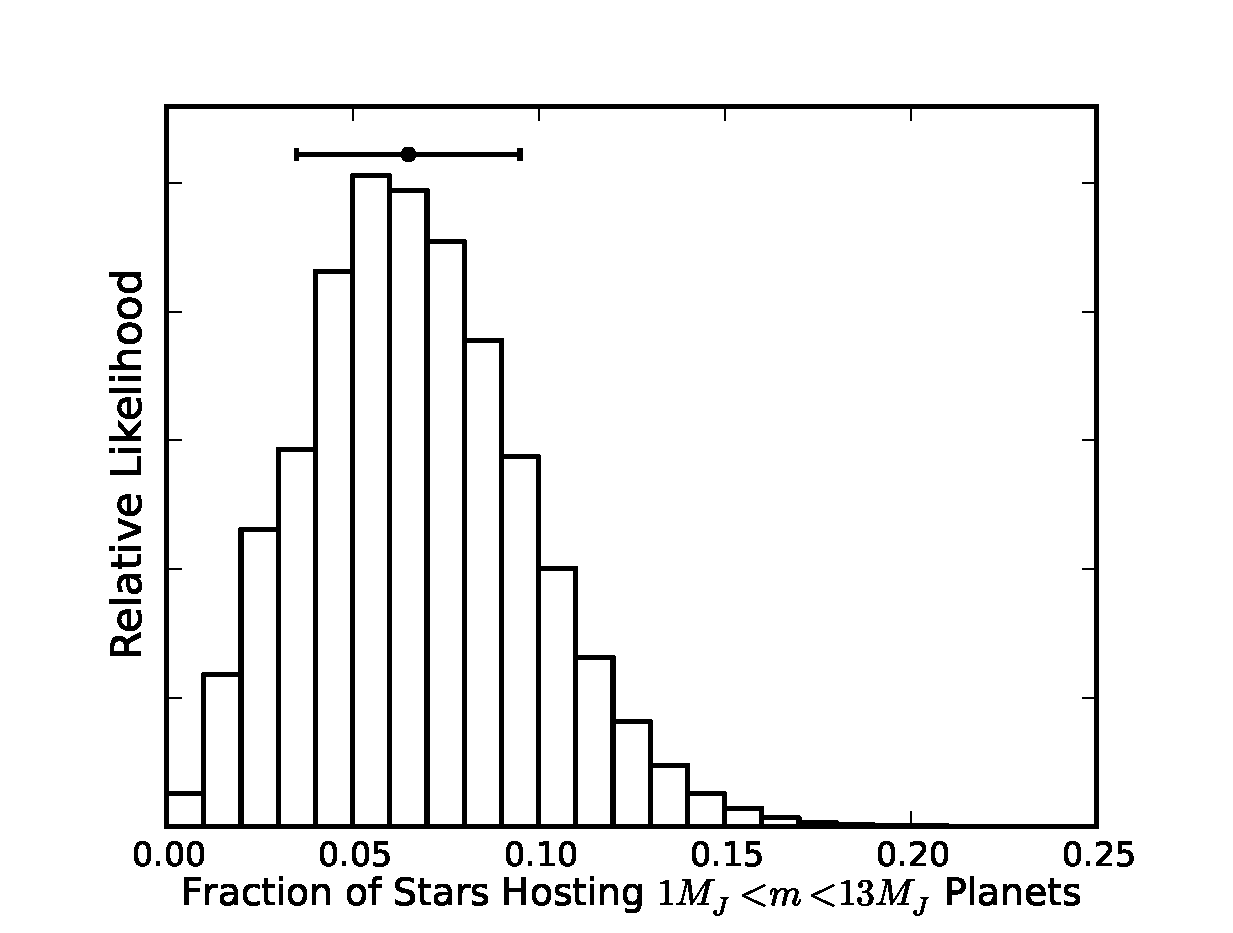
\includegraphics[width=0.75\textwidth]{chapter3/f9.eps}}
\caption[Posterior distribution of the occurrence rate of giant planets
orbiting M dwarfs]{Giant planet occurrence for our sample of 111 nearby M-dwarfs. We find $6.5\% \pm 3.0\%$ of M-dwarfs host a planet with mass $1 M_J < m < 13 M_J$ and $0 < a < 20$ AU.}
\label{HistoResult}
\end{figure}

This is the first study using observed RV accelerations to estimate the giant planet occurrence rate. However, previous RV studies have discussed the presence or nondetection of RV accelerations in their analysis. For example, \citet{Endl03} mentioned all RV accelerations in their sample are likely the cause of stellar binaries. Our observations are generally more precise than theirs, as we detect some planets that they miss (such as Gl 436 and Gl 849).

\citet{Bonfils13} detect 15 long-term accelerations in their sample of 102 southern M-dwarfs. Some of these can be attributed to long period binary companions (such as Gl\,250B and Gl\,618A). Of the stars where we detect an RV acceleration, only one (Gl\,849) is in the HARPS sample; these authors also detect an acceleration. \citet{Bonfils13} also detect an acceleration around Gl\,699 (Barnard's star) that we do not detect. Such an acceleration has also not been found by other studies: \citet{Choi13} claim the RV of Barnard's star is increasing at $4.515 \pm 0.002$ m s$^{-1}$ yr$^{-1}$, consistent with the expected secular acceleration but inconsistent with the $-3.043 \pm 0.646$ m s$^{-1}$ yr$^{-1}$ acceleration observed by \citet{Bonfils13}. With more observations over a longer time baseline, this discrepancy will be resolved.



\subsection{Potential Missed Binary Stars}
\label{PMBS}
We only collect AO images for systems with long term RV accelerations. For these accelerations to be observable, the orbiting companion must have a component of its movement along our line of sight so that the radial velocity changes during an orbit. A giant planet would be missed if it was in a near face-on orbit, such that the star's reflex motion was primarily in the plane of the sky. Such systems are accounted for in our detectability calculations (Figure \ref{Detectability}), as we have determined the probability of detecting a planet's RV acceleration as a function of its mass and separation, marginalized over all other orbital parameters. These calculations do not, however, account for the possible presence of close stellar binary companions in face-on orbits. Although less common than edge-on systems, any missed binary systems that we have not rejected from our sample would cause our planet occurrence rate to be artificially low (assuming these systems could not form dynamically stable planets). Close binaries would be observable as double-lined spectroscopic systems (SB2s) in the CPS data, while wider binary pairs would be easily imaged by AO systems.

The RV sample was originally selected to reject systems with known binary companions within 2 arcseconds. We would expect companions with a flux ratio larger than 0.01 ($\Delta V = 5$) to be detected as binaries \citep{Robinson07}. For our brightest targets, this would correspond to M6 dwarfs and brighter. As the cutoff for hydrogen burning is the M6 spectral class \citep{Luhman12}, we would expect all close stellar-mass binaries to be removed from our HIRES observations. 

To determine how many missed binaries are in our sample, we simulate a population of binary companions to M-dwarfs. We create binary companions such that their semimajor axes are assigned following the observed distribution found by \citet{Fischer92}. We randomly assign the other orbital parameters and determine there is a $41.8\% \pm 0.3\%$ chance a binary companion in our sample around a random star would have a projected separation smaller than two arcseconds. Thus, considering \citet{Fischer92} find $42\% \pm 9\%$ of local M-dwarfs are in binary or multiple systems, we would expect to have a total of $24 \pm 6$ binary systems in our sample, which originally contained 137 stars before the removal of known binaries. As we actually observe 22 binary systems (containing 26 stars), this result is consistent with our expectation.

We then determine the radial velocity each simulated binary star would induce on our host companion. For each binary that induces a measurable acceleration on the host star, we simulate imaging observations to determine the probability this binary companion would be detected in either our AO survey or, for very wide separation binaries, a seeing-limited ground based survey such as 2MASS. By applying our joint AO/seeing-limited contrast curves, we find that if a binary star system in our survey induces an RV acceleration, we would have a $96.0\% \pm 0.4\%$ chance of imaging this binary companion. Therefore the probability that one or more of our observed accelerations is caused by a ``missed'' binary companion is negligible and this possibility does not significantly affect our results.




\subsection{Dependence on Stellar Mass}
\label{MassDep}
Previous RV studies have found a correlation between stellar mass and giant planet occurrence at $a < 2.5$ AU, with more massive stars more likely to host giant planets \citep{Johnson10a}. To test this relation inside the M-dwarf spectral class, we analyzed the high mass stars separately from the low mass stars in our sample. From our best fit masses, half of our sample is more massive than $M = 0.41 M_\odot$. We thus use this value as a dividing line to separate our sample into two groups. Our masses have typical uncertainties of $10\%$, so for each star, given its mass and uncertainty, we determine the probability it is larger or smaller than $0.41 M_\odot$ assuming normally distributed errors. We then use that value as a weighting factor to assign a probability for each individual star to reside in our high mass or low mass bin, and then repeat our analysis for each individual subsample.

We find an occurrence rate for the high mass subsample of $4.8 \pm 3.3\%$ and for the low mass subsample of $7.9 \pm 4.2\%$ (Figure \ref{Mass}). \citet{Johnson10a} find planet occurrence is correlated with stellar mass such that $f_{pl} \propto 10^{(1.2\pm 0.2)\textrm{[Fe/H]}}M_\star^{(1.0\pm 0.3)}$. The average star in our high-mass sample has a mass of 0.5 $M_\odot$ while the average star in our low-mass sample has a mass of 0.3 $M_\odot$, so we would expect the high-mass subsample to have an occurrence rate larger than the low-mass sample by a factor of 1.67. We find the true occurrence rate to change by a factor of $0.61 \pm 0.87$ in moving from the lower-mass to higher-mass bin. This is inconsistent with the expected result from \citet{Johnson10a}, but the difference between the two bins is not significantly different from zero. A larger sample is required to determine if the small difference between these two populations of M-dwarfs is real or the result of a statistical anomaly. However, our result is lower than the \citet{Cumming08} result for FGK stars, that $f_{pl} = 10\% \pm 1\%$ of FGK stars host Jupiter-mass planets within 20 AU. This difference is consistent with the \citet{Johnson10a} correlation between stellar mass and planet occurrence. 


\begin{figure}[htbp]
\centerline{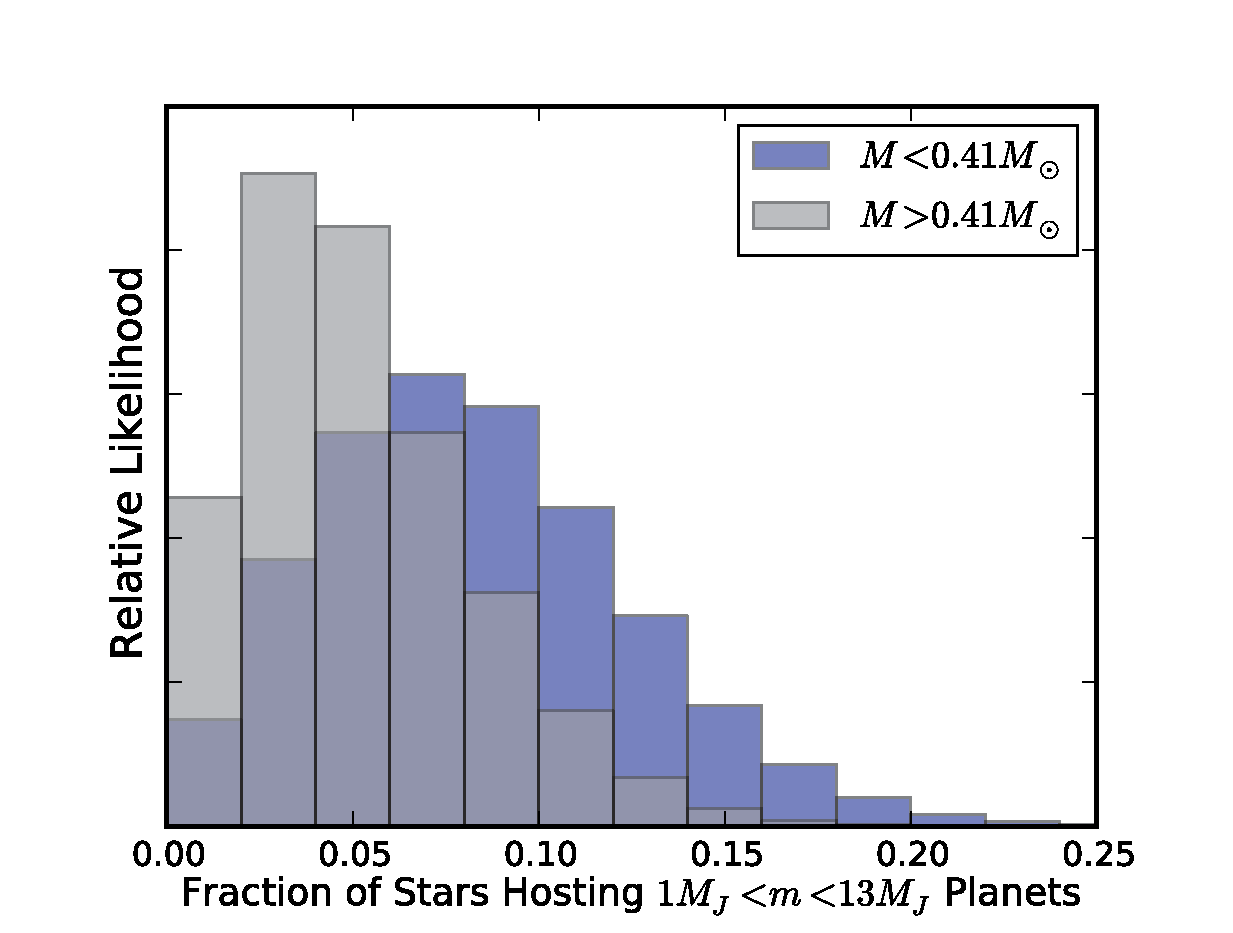
\includegraphics[width=0.75\textwidth]{chapter3/f10.eps}}
\caption[Posterior planet occurrence for a high-mass and low-mass
subpopulation of M dwarfs]{Planet occurrence for a low mass subsample (blue) and a high mass subsample (gray) of M dwarfs. Both subsets have nearly similar giant planet occurrence rates, suggesting planet occurrence may not depend strongly on stellar mass within the M spectral class. A larger sample is required to determine if the lack of difference in occurrence rates is astrophysical or statistical variance.
  }
\label{Mass}
\end{figure}



\subsection{Dependence on Metallicity}
\label{MetalDep}
Previous RV studies of giant planets have also found evidence for a correlation between planet occurrence and metallicity \citep{Fischer05, Johnson10a}. To test if this correlation holds for more distant planets, we again split our sample into two, using the same method from the previous section. In this case, we use [Fe/H] $= -0.10$, the sample median metallicity, as the dividing line for our subsamples. We assume all stars have metallicity uncertainties of 0.17 dex, consistent with the scatter expected from the \citet{Neves12} empirical relation. Again, we assume Gaussian errors to determine the probability each star is in a specific subsample. We then repeat our analysis on both groups.

\begin{figure}[htbp]
\centerline{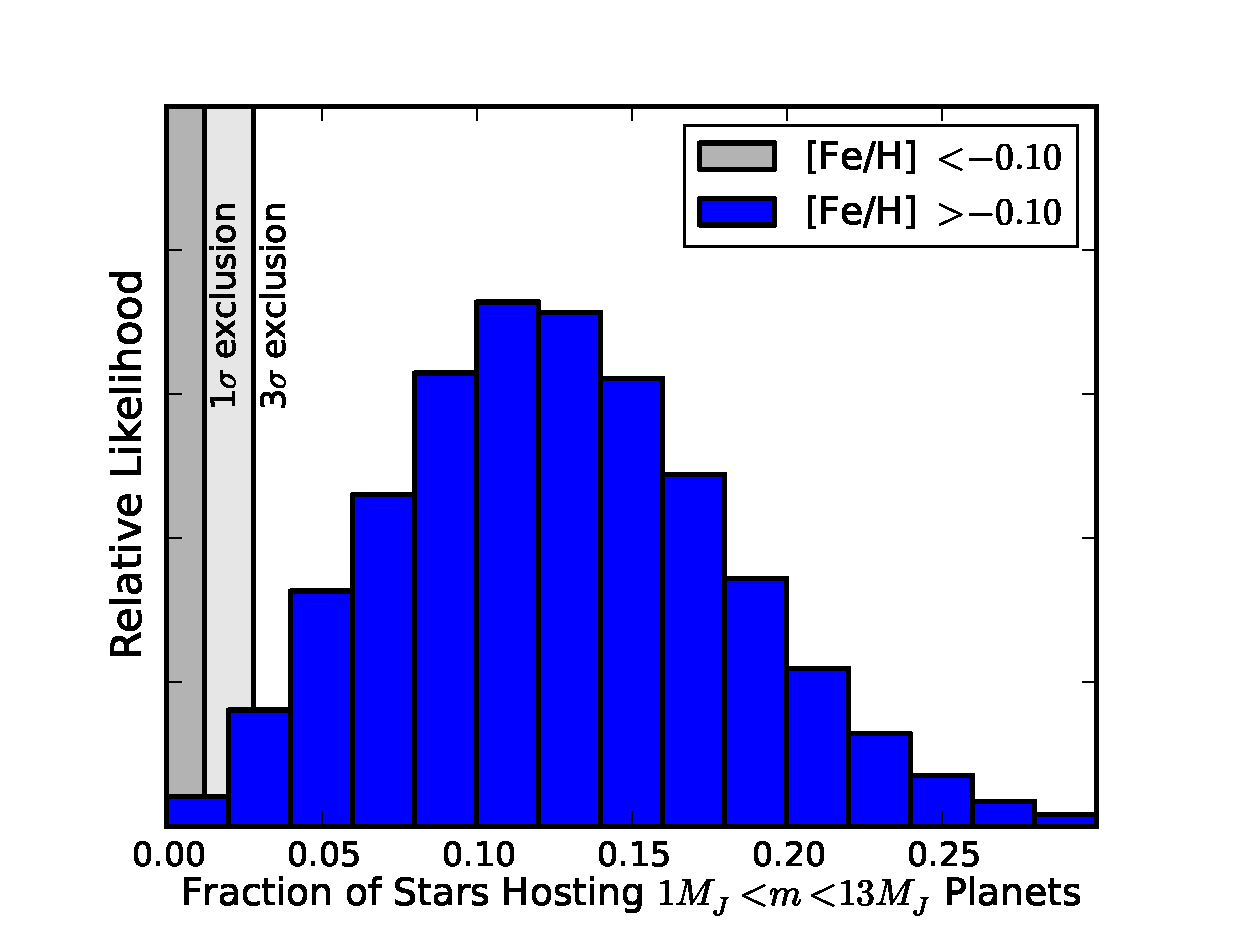
\includegraphics[width=0.75\textwidth]{chapter3/f11.eps}}
\caption[Posterior planet occurrence for a high-metallicity and low-metallicity
subpopulation of M dwarfs]{ Planet occurrence for a high metallicity subsample (blue) and 1$\sigma$ and 3$\sigma$ exclusion regions for a low metallicity subsample (gray) of M dwarfs. In the low metallicity subsample, we are able to rule out planet occurrence rates larger than 1.2\% at $1\sigma$ and 2.8\% at $3\sigma$, represented by the labeled vertical lines. The high metallicity sample has a significantly higher occurrence rate than the low metallicity sample, similar to the phenomenon observed for RV-detected planets at smaller separations. 
  }
\label{Metals}
\end{figure}
In the high-metallicity subsample, we find an occurrence rate such that $12.4 \pm 5.4\%$ of M-dwarfs host giant planets. In the low metallicity sample the occurrence rate drops to $0.96 \pm 0.51\%$. In Figure \ref{Metals} we plot a histogram of our posterior distribution of planet occurrence for our high-metallicity subsample. Vertical lines represent (from left to right) 1$\sigma$ and 3$\sigma$ upper limits on the planet occurrence rate for the low-metallicity subsample. From these distributions, the giant planet occurrence rate for metal-rich stars has only a $2.4\%$ probability of being lower than the $3\sigma$ upper limit on the planet occurrence rate for metal-poor stars. The difference between these subsamples may be suggestive of the same effect seen for RV-confirmed planets within 2.5 AU \citep{JohnsonApps09, KOI254}. 


An increase in the planet occurrence rate with metallicity for planets beyond a few AU may suggest giant planets in wide orbits are commonly formed by the same processes as the RV giant planet population. This study will be facilitated by the development of reliable spectroscopic metallicity measurements \citep{RA10}.


\subsection{The Stellar Mass-Metallicity Plane}
We can quantify our giant planet occurrence rate with respect to stellar mass and metallicity. Such an approach has been undertaken for planets with $a < 2.5$ AU orbiting stars of all spectral types previously \citep{Johnson10a}; we follow the techniques of these authors but confine ourselves to strictly giant planets in the range $0 < a < 20$ AU orbiting stars of the M-dwarf spectral class.

We assume that stellar mass and metallicity produce separate effects on the giant planet occurrence rate, so that the fraction of stars with planets as a function of mass and metallicity can be written as a double power-law,
\begin{equation}
f(M,F) = CM^a10^{bF},
\end{equation}
where $C$, $a$, and $b$ are constants, $M \equiv M/M\odot$, and $F \equiv$ [Fe/H].

In this analysis, we have a binary result: a star either has a giant planet, detectable as an RV acceleration or closed orbit, or it does not. Therefore, each of the $N$ stars in our sample represents a Bernoulli trial. Given $T$ total observed giant planets, if we assume the probability of a Doppler detection of a giant planet around any given star $i$ is $f(M_i, F_i)$, then by Bayes' theorem, the probability of a given model $X$ given our data $d$ is
\begin{equation}
P(X|d) \propto P(X) \prod_i^T f(M_i,F_i) \times \prod_j^{N-T} [1- f(M_j,F_j)].
\label{Likeli}
\end{equation}

Our measurements of stellar masses and metallicities are imperfect. Therefore, we treat the masses and metallicities of these stars as probability distributions. We consider each star's mass and metallicity distribution to be a two-dimensional Gaussian with mean {$M_i,F_i$} and standard deviation {$\sigma_{M,i},\sigma_{F,i}$ and call this term $p$. In this case, the predicted planet fraction for a star with mass $M_i$ and metallicity $F_i$ is
\begin{equation}
f(M_i,F_i) = \int \int p(M_i, F_i)f(M,F)dM dF.
\end{equation}
We can thus apply Eq. \ref{Likeli} with varying parameters, $X = {C, a, b}$, to maximize $\mathcal{L}$ conditioned on the data. We elect to use uniform priors, instead of applying the results of previous studies as a prior. \citet{Johnson10a} and \citet{Mortier13} study a sample of stars including all stellar types F to M, so their results may not represent our population well. More recent studies, such as \citet{Neves13}, are restricted to M-dwarfs. However, while their techniques are similar, they only attempt to constrain metallicity, implicitly assuming $a=0$. Additionally on of the three detected planets in their sample is a planet smaller than Jupiter around a metal-poor star. As our sample is limited to planets larger than Jupiter, the resultant distribution found by these authors may not be representative of the population of giant planets ($m > 1 M_J$).}

We find our giant planet fraction is described by the distribution function
\begin{equation}
f(M,F) = 0.039^{+0.056}_{-0.028} M^{0.8^{+1.1}_{-0.9}} 10^{(3.8 \pm 1.2)F}.
\end{equation}
The $1\sigma$ confidence interval for $C$ is highly skewed, while the other two parameters are approximately normally distributed. In Figure \ref{Covar}, we plot the marginal posterior probability distribution functions for each pair of parameters. Perhaps not surprisingly, we find a covariance between $C$ and $b$. Because our metallicity parameter $b$ is so steep, small changes in $b$ must cause changes in $C$ to keep the giant planet fraction consistent at a given metallicity.

\begin{figure}[htbp]
\centerline{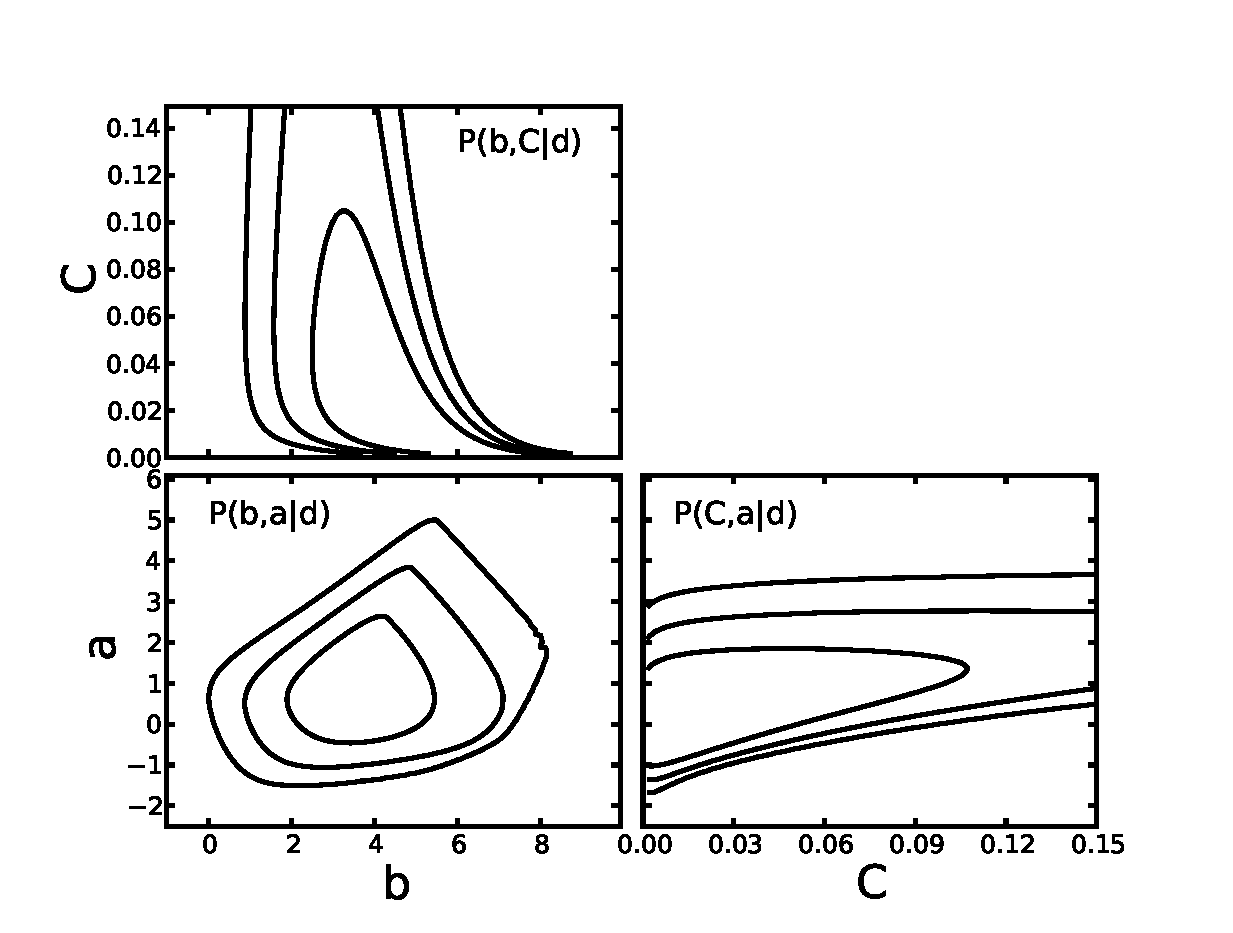
\includegraphics[width=0.75\textwidth]{chapter3/f12.eps}}
\caption[Marginal posterior distributions for the planet population model as a function of allowed power-law parameters]{Marginal posterior pdfs for the planet population model conditioned on our M-dwarf data. We find, as by other methods in previous sections, that giant planet occurrence is a strong function of stellar metallicity, but may not depend strongly on stellar mass inside of the M spectral class. 
  }
\label{Covar}
\end{figure}

Our results are steeper in $b$ than \citet{Neves13}, although the giant planet occurrence rates at [Fe/H] $\sim 0.1$ are consistent between the two studies. This is likely due to the inclusion of a planet with a minimum mass of 0.7 Jupiter masses in the ``Jovian'' sample of these authors. This planet orbits a star with a metallicity [Fe/H] $= -0.19 \pm 0.08$, flattening the distribution with metallicity. The fact remains that, while the metallicity distribution of field stars is centered near [Fe/H] $=0.0$ with a standard deviation of 0.13 dex, there are presently no giant planets orbiting M-dwarfs with measured metallicities smaller than +0.08 in either the HARPS or HIRES sample. The giant planet distribution function must therefore be a strong function of stellar metallicity. Moreover, it is essential to develop improved methods to measure metallicities of low-mass stars, such as the techniques developed by \citet{RojasAyala12} and \citet{Mann13a}.


\subsection{The Effect of Distant Binary Companions}

In the above analysis, we neglect binary stars where a test particle at 30 AU would be in an unstable orbit, but include 14 binaries at wider separations. Although these systems formally allow stable orbits, \citet{Kaib13} suggest these orbits can change significantly over time. Because the binary pair is weakly bound, interactions with the galactic tidal field or nearby passing stars can vary the binary orbit. The binary can then strongly perturb formerly stable planetary companions, potentially resulting in the ejection of planets from the system within 5 Gyr, our estimated age for the M-dwarfs in our sample. None of our 10 wide binary systems show evidence for an RV acceleration, providing weak but tantalizing evidence in favor of this theory. If we repeat our analysis but neglect these stars as potential hosting systems, we find that $7.4\% \pm 3.3\%$ of single stars host giant planets, compared to $6.5\% \pm 3.0\%$ of our full sample. With zero detections in a sample of 14 wide binaries, we can only place an upper limit of $f_{pl} \leq 0.20$ at $95\%$ confidence on the occurrence rate of giant planets in wide binary systems. With more observations of stars with wide binary companions, the occurrence rate of planets orbiting true field stars can be compared to the rate for wide binaries.



\subsection{Sensitivity to Power-Law Parameters}
\label{PL}
The result for $f_{pl}$ is dependent on the exact parameters of the planetary distribution function, as that function determines the number of missed (false negative) planets in our sample. To quantify the dependence of the planetary occurrence rate on our choice of $\alpha$ and $\beta$ we repeat our analysis over a grid of values for $\alpha$ and $\beta$. The giant planet occurrence rate as a function of these two parameters is shown in Figure \ref{AlpBetOcc}. We find that there is only a weak relation between $\alpha$ and $f_{pl}$ in the range $-2.0 < \alpha < 0.5$, where we might reasonably expect $\alpha$ to reside. $f_{pl}$ depends more strongly on $\beta$, but our overall result does not change by more than $1\sigma$ by selecting any $\beta$ in the range $-1.0 < \beta < 1.0$ for a given $\alpha$. Selecting any $\alpha$ or $\beta$ over this range affects our final result by less than a factor of two.

\begin{figure}[htbp]
\centerline{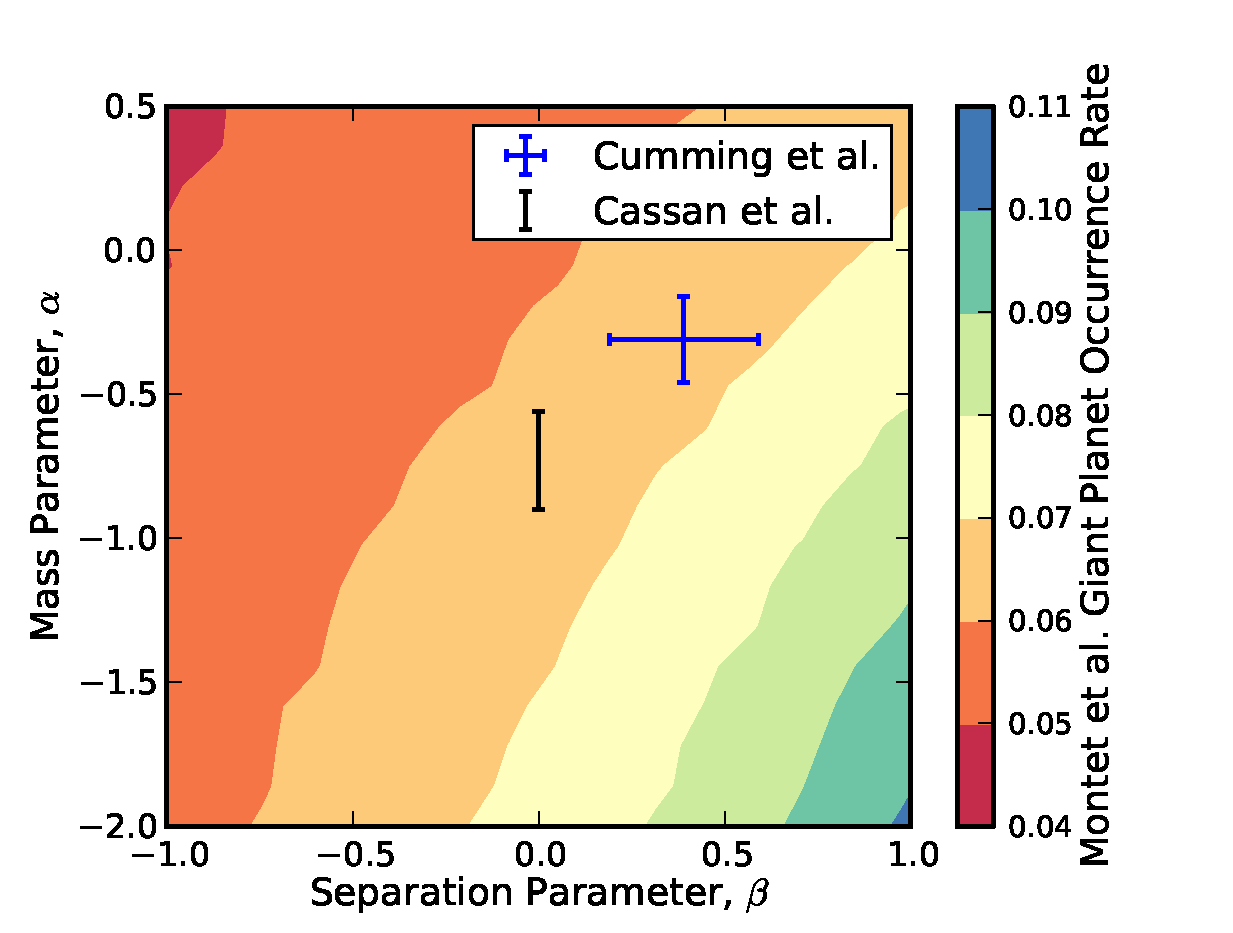
\includegraphics[width=0.75\textwidth]{chapter3/f13.eps}}
\caption[Calculated giant planet occurrence rate, $f_{pl}$, as a function of the mass parameter index $\alpha$ and separation parameter index $\beta$]{Calculated giant planet occurrence rate, $f_{pl}$, as a function of the mass parameter index $\alpha$ and separation parameter index $\beta$. There is not a strong dependence on $\alpha$ or $\beta$; selecting $\alpha < -1.0$ and $\beta > 0.5$ is required to affect our result at more than the $1\sigma$ level. Labeled points include the \citet{Cumming08} result for FGK stars, with $\alpha = -0.31 \pm 0.15$ and $\beta = 0.39 \pm 0.15$, and the microlensing result of \citet{Cassan12}, who find $\alpha = -0.73 \pm 0.17$ and assume $\beta \equiv 0$.
  }
\label{AlpBetOcc}
\end{figure}


From our sample of targets alone, we are unable to place constraints on acceptable values of $\alpha$ and $\beta$. To constrain $\alpha$ and $\beta$, the occurrence rate of giant planets at a given mass or separation is required. We have determined the bulk occurrence rate of planets, but cannot uniquely determine their properties. With continued observations, as our RV accelerations ``turn over'' and become closed orbits, we will be able to determine the exact locations of giant planets around M-dwarfs and constrain the power-law parameters. Alternatively, we can constrain $\alpha$ and $\beta$ by combining our results with those from microlensing observations.


\subsection{Comparison with Microlensing Results}
\label{muL}
 
In \textsection\ref{PL}, we showed that our bulk occurrence rate is not a strong function of $\alpha$ and $\beta$. However, the types and locations of our planets is a function of these parameters: if $\alpha$ is large, then most of our observed trends must be caused by large planets in wide orbits. Since microlensing results are most sensitive at projected separations corresponding to the Einstein radius, where $R_E \sim 3.5 \textrm{AU} (M_\star/M_\odot)^{1/2}$, we can compare our results to microlensing planet occurrence studies. As our results will only be consistent with microlensing estimates of the planet occurrence rate at the Einstein radius for specific values of $\alpha$ and $\beta$, comparisons between the two methods will enable us to constrain $\alpha$ and $\beta$. 

To compare the two sets of results, we assume the population of M-dwarfs observed by microlensing studies is similar to that targeted by RV surveys in the local neighborhood.  We find evidence for a correlation between giant planet frequency and metallicity in our sample, similar to that found by previous RV analyses of planets with $a < 2.5$ AU \citep{Fischer05, JohnsonApps09}. M-dwarfs studied by microlensing are at distances larger than 1 kpc and in the direction of the galactic bulge, along the galactic metallicity gradient \citep{Rolleston00}. Measurements of the metallicity of Cepheids suggest the iron content in the disk varies such that $d\textrm{[Fe/H]}/dr = -0.051 \pm 0.004$ dex kpc$^{-1}$ between 5 and 17 kpc from the galactic center \citep{Pedicelli09}. Thus, the microlensing M-dwarfs may be more metal-rich than stars in the local neighborhood, so $f_{pl}$ may be larger for the microlensing population than the RV population. Without spectra of galactic stellar planet-hosting lenses their true stellar properties are unknown. Programs dedicated to collecting spectra of galactic stellar planet-hosting lenses would greatly inform our knowledge of these stars and their planets.

If we assume the planet mass distribution function of \citet{Cumming08}, then from our analysis we would expect microlensing studies to measure a planet occurrence rate $f_{pl} = 0.056 \pm 0.023$ bound Jupiter-mass planets per star by analyzing signals from planets near the Einstein radius. \citet{Cassan12} claim an occurrence rate of $10^{-0.62\pm0.22}$ ($0.24^{+0.16}_{-0.10}$) Saturn-mass planets at this separation. If we scale this occurrence rate to Jupiter-mass planets following the mass index observed in microlensing studies, $\alpha = -0.73 \pm 0.17$, then the observed microlensing density of Jupiter mass planets would be $0.101 \pm 0.016$ planets per star, different from our expectation at $1.6\sigma$.  If (and only if) the two populations have intrinsically similar occurrence rates of giant planets, then the difference between the number of planets found must be due to a planet distribution different from the one used by \citet{Cumming08}. As the RV planet distribution was developed from an analysis of FGK stars, while the microlensing population generally consists of M dwarfs that may be preferentially metal-rich compared to stars in the local neighborhood, it may not be surprising if the RV planet population is intrinsically different from the microlensing planet population.

\subsubsection{Joint Constraints on $\alpha$}

We depart from our previously assumed values of $\alpha$ and $\beta$ to determine what values of $\alpha$ and $\beta$ satisfy both our observed RV accelerations and the results of \citet{Cassan12}. We assume the planet occurrence rate presented by \citet{Cassan12} is representative of the planet population at the Einstein radius. Moreover, we assume planet orbital semimajor axes are distributed uniformly in logarithmic space following \"Opik's Law ($\beta = 0$), as microlensing studies assume. This is slightly shallower than what is observed in the RV planet population ($\beta = 0.39 \pm 0.15$), but since the RV population of giant planets likely underwent considerable migration this may be a reasonable assumption. We then vary $\alpha$, and for each value determine the space density of planets at 2.5 AU. We then compare our expected result to the result from \citet{Cassan12}, which we scale to Jupiter-mass planets according to our $\alpha$ parameter. We finally require $\alpha < 0$: despite the uncertainties in this mass parameter, previous studies agree that around M dwarfs, small planets are more common than massive planets \citep{Swift13, Morton14}. 

We find microlensing results agree with our result for $f_{pl}$ when $\alpha = -0.94 \pm 0.56$ (Figure \ref{alphaopik}). This result is consistent with the best-fitting values for $\alpha$ found by \citet{Gould10} and \citet{Cassan12}. If we include the \citet{Cassan12} result as a prior in our analysis, we find $\alpha = -0.77 \pm 0.22$. However, while our result agree with microlensing studies, our result for $\alpha$ is different from the \citet{Cumming08} result for FGK stars at $1.1 \sigma$ and significantly different from the \citet{Bowler10} constraints for A stars, which rule out all $\alpha < 0.25$ with 90\% confidence and all $\alpha < 1.75$ with 50\% confidence. Since microlensing predicts a larger number of planets found at the Einstein radius relative to that expected by RV extrapolations, it is not surprising that we find a smaller value for $\alpha$ is required for our result to be consistent with the microlensing results: if the two populations are the same, there must be many low-mass giant planets below the simultaneous RV and imaging detectability limits than high-mass planets above the limits.

\begin{figure}[htbp]
\centerline{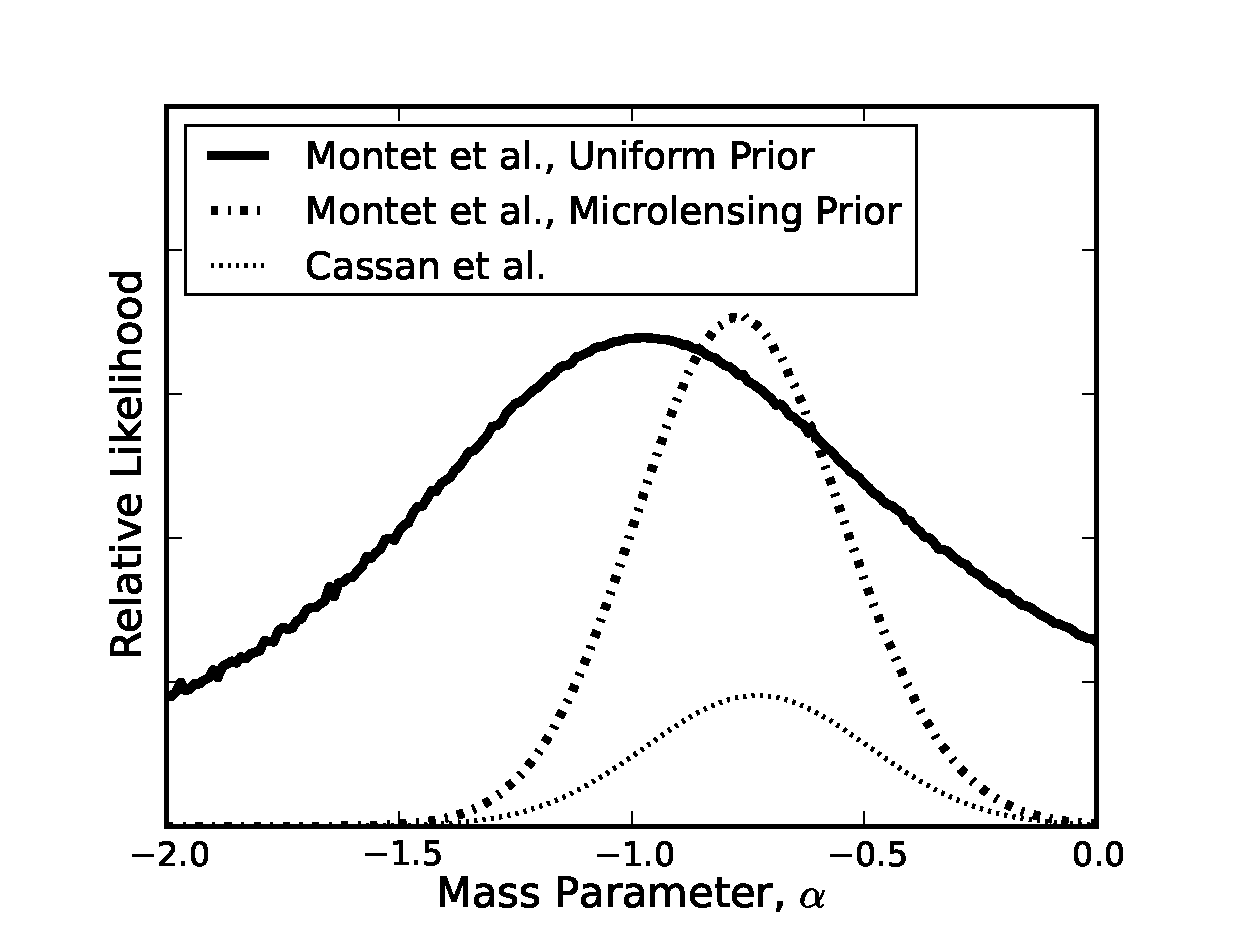
\includegraphics[width=0.75\textwidth]{chapter3/f14.eps}}
\caption[Relative likelihood values for the mass parameter $\alpha$, assuming the planets in our sample and microlensing systems are members of the same population]{Relative likelihood values for the mass parameter $\alpha$, assuming the planets in our sample and microlensing systems are members of the same population. We find a maximum likelihood value of $\alpha = -0.94 \pm 0.56$, consistent with values of $\alpha$ found from analyses of microlensing planets but steeper than previous RV results for FGK stars at $1.1 \sigma$. This result may suggest the planet distribution function is different for M stars as compared to higher mass stars. When we include the \citet{Cassan12} result as a prior on our measurement, we find $\alpha=-0.77 \pm 0.22$.
  }
\label{alphaopik}
\end{figure}

\subsubsection{Simultaneous Constraints on $\alpha$ and $\beta$}

We are not restricted to \"Opik's Law. We can allow both $\alpha$ and $\beta$ to vary, and compare the normalization of \citet{Cassan12} for Saturn-mass objects at 2.5 AU to our projected planet density at that mass and separation (Figure \ref{alphabeta}). Performing this exercise, we find the most acceptable values of $\alpha$ and $\beta$ are correlated approximately along the line $\alpha - \beta = -1$. That is, for every 1 dex increase in $\alpha$, $\beta$ must decrease by 1 dex to maintain a reasonable fit to both our result and the microlensing results. 

\begin{figure}[htbp]
\centerline{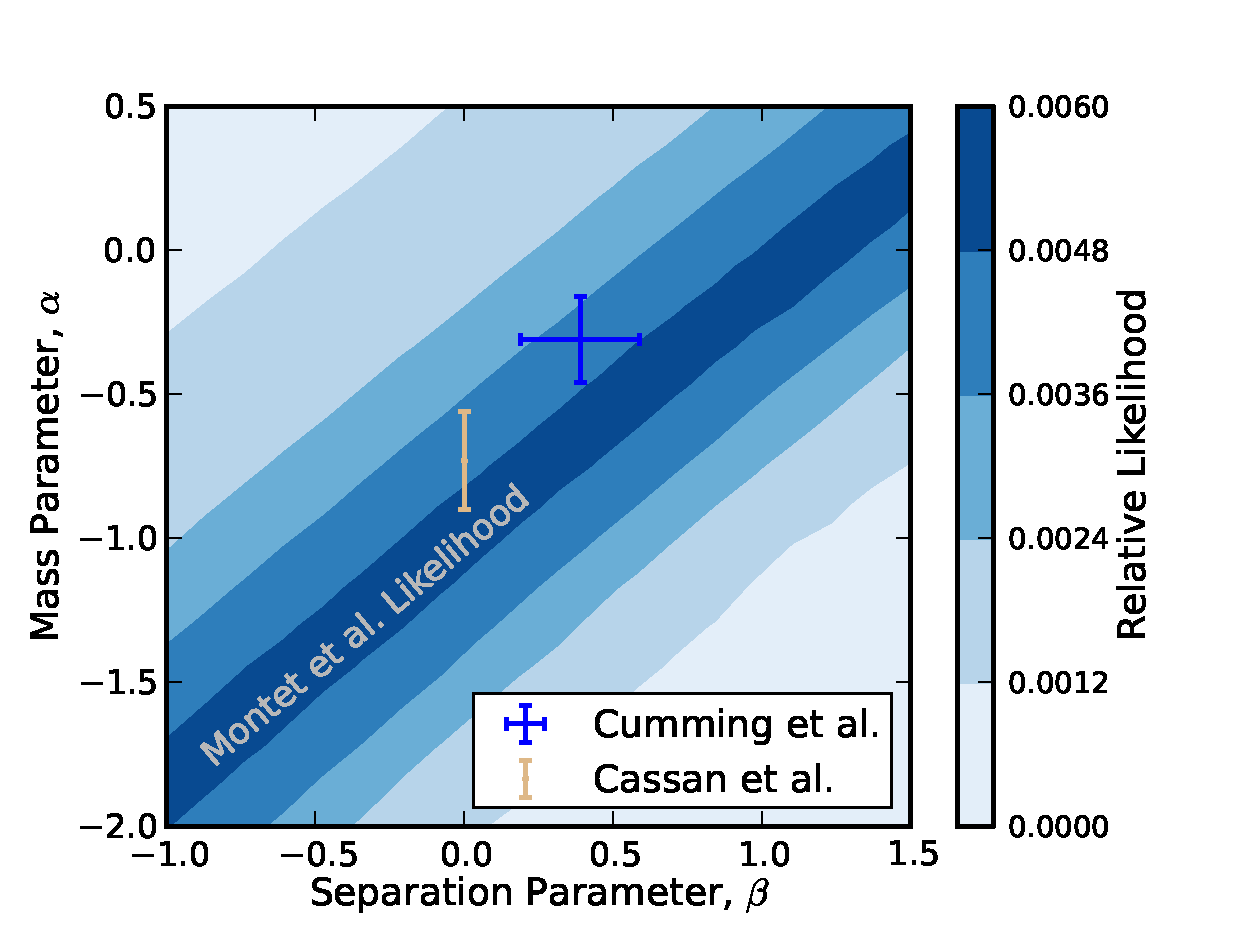
\includegraphics[width=0.75\textwidth]{chapter3/f15.eps}}
\caption[Relative likelihood values for the mass parameter $\alpha$ and separation parameter $\beta$]{Relative likelihood values for the mass parameter $\alpha$ and separation parameter $\beta$. There is a maximum likelihood contour approximately along the line $\alpha - \beta = -1$, suggesting a relationship between the two parameters required to fit both our result and the microlensing results, assuming the local planets in our sample and microlensing systems are members of the same population. Points included in the plot are the \citet{Cumming08} RV result (blue) and the \citet{Cassan12} microlensing result (cyan), the latter of which assumes an \"Opik's Law value of $\beta = 0$. The small discrepancy between our result and the \citet{Cumming08} result may suggest the planet distribution function may differ between M-dwarfs and FGK stars.
}
\label{alphabeta}
\end{figure}

\subsubsection{A Model-Independent $f_{pl}$}
We can apply these relative likelihood values as priors to the occurrence rate as a function of $\alpha$ and $\beta$ shown in Figure \ref{AlpBetOcc} to determine an occurrence rate independent of our choices of $\alpha$ and $\beta$, but dependent on the RV and microlensing stars both being representative of similar populations. We assume our separation parameter must be in the range $-1.0 < \beta < 1.0$, consistent with the assumptions from previous microlensing studies, and allow our mass parameter to be any value subject to the constraints of Figure \ref{alphabeta}. By weighting our occurrence rates found in \textsection\ref{PL} in this manner, we find a most likely occurrence rate of $7.2 \pm 3.1\%$, consistent with that found by assuming the power-law distribution of \citet{Cumming08}. As the measured planet frequency depends on the distribution function parameters, an improved value of the planet occurrence rate, either by this method, microlensing, or through astrometry measured by \textit{Gaia} \citep{Casertano08}, will provide immediate constraints on the distribution function of giant planets. Similarly, improved constraints on the distribution parameters will enable an immediate improvement of the determination of the giant planet occurrence rate.

The \citet{Cumming08} power-law parameters $\alpha$ and $\beta$ are less consistent with our results. This may suggest the planet distribution function around FGK stars is systematically different from the planet distribution function around M-dwarfs. As \citet{Bowler10} find an even larger value for $\alpha$ in their study of retired A stars (excluding all $\alpha < 0$), which matches comparison studies between RV surveys and high-contrast imaging searches \citep{Crepp11}, this possibility is certainly plausible. With additional M-dwarfs targeted by a combination of RV observations with longer time baselines and high-contrast imaging to improve the estimate of the occurrence rate, we will be able to directly probe this possibility.




\section{Summary and Conclusion}
\label{SC}
We have analyzed a collection of 111 nearby M-dwarfs observed in RV surveys with a median time baseline of 11.8 years in a search for long-term RV accelerations. We have developed a new technique to determine the incidence of giant planets in which we target systems with such accelerations using adaptive optics imaging to ``peer beyond the horizon'' set by Doppler time baselines. With a relatively short exposure image using the Keck AO system, we can eliminate the possibility of binary stellar companions and massive brown dwarfs. We conclude with high statistical confidence that accelerations without a directly imaged companion are likely caused by a planet in a wide orbit. 

Accounting for false positive and false negative rates, we find that $6.5 \pm 3.0\%$ of M-dwarfs host a giant planet with mass $1 < m / M_J < 13 $ and semimajor axis $0 < a < 20$ AU, assuming such planets are distributed following the power-law parameters estimated by \citet{Cumming08}. The exact integrated planet occurrence rate does not depend strongly on the distribution function parameters chosen. We find evidence for a correlation between giant planet frequency and stellar metallicity, similar to that observed in the RV-detected planet population. Additional follow-up work confirming this result would suggest giant planets in wide orbits may form in the same way as the RV-detected giant planets. Observations of more stars are needed to determine if a correlation exists between planet occurrence at wide separations and stellar mass inside of the M-dwarf spectral class. 

Our overall occurrence rate is consistent with what might be expected based on the results of microlensing planet search surveys. However, if the giant planet distribution is given as a double power law similar to that found by \citet{Cumming08}, such that $d^2N \propto M^\alpha a^\beta d\ln M d\ln a$, with $\alpha = -0.31 \pm 0.20$ and $\beta = 0.39 \pm 0.15$, where $\alpha$ and $\beta$ are planet distribution power-law indices defined in Eq. \ref{DPL}, then microlensing studies overestimate the giant planet occurrence rate. From our bulk occurrence rate, we determine an expected planet detection rate for microlensing studies which depends on our chosen planet distribution function. By assuming an \"Opik's Law distribution (i.e., flat in $\log a$), the microlensing planet occurrence rate is consistent with our result if the planet population is represented by the power-law $dN \propto m^{-0.94 \pm 0.56} d\log m$. This value for $\alpha$ is consistent with previous M-dwarf studies conducted by microlensing planet search teams \citep{Gould10, Cassan12}. We also find other non-\"Opik distributions can be chosen to simultaneously explain our results and the microlensing results; these fall approximately on the line $\alpha - \beta = -1$. Moreover, an improved estimate of the giant planet occurrence rate, as measured by \textit{Gaia}, can be combined with our results to provide enhanced constraints on $\alpha$ and $\beta$.  

Our knowledge of planets around M-dwarfs has significantly improved in the last few years thanks to both targeted RV searches and high contrast imaging campaigns \citep{Apps10, Bowler12a}. As such surveys continue, they will begin to confirm and characterize planets in wider orbits, pushing into the domain currently only studied by microlensing studies. To directly compare these populations, understanding the properties of host stars to planets found by microlensing will be extremely important; when possible, every effort should be made to collect spectroscopic followup data on microlensing events to determine the physical properties of lens host stars to better understand both the planet population around M-dwarfs and how it changes across the galaxy.

The method developed in this paper can be extended to higher-mass stars with little difficulty. For example, a large sample of K-dwarfs has been observed by the CPS collaboration. This sample is larger, has more observations, and exhibits less astrophysical jitter than our M-dwarf sample; all of these factors improve our ability to detect RV accelerations. However, the stars are more luminous and on average more distant, complicating adaptive optics searches. Care must be taken to ensure low-mass stellar companions are accounted for, as adaptive optics imaging may not be sensitive to all M-dwarf companions to K-dwarfs without longer observations or the use of ADI. In the future, we intend to apply this technique to the CPS K-dwarfs to determine the planet occurrence rate around higher mass stars and compare to the M-dwarfs.

\begin{landscape}
{\footnotesize
\begin{longtable}{l|cccccccccccc} 
\hline
Star & RA & Dec & Mass ($M_\odot$) & [Fe/H] & Spectral Type & $V$ & $V$ Source & d (pc) \\
\hline
    Hip 428 & 00:05:10.9 & +45:47:11.6 & 0.53 & -0.07 & M1 &  9.93 & \citet{Gliese91} & 11.25  \\ 
    HD 225213 & 00:05:24.4 & -37:21:26.5 & 0.39 & -0.42 & M1.5 &  8.57 & \citet{Koen10} &  4.34  \\ 
   Hip 1734 & 00:21:56.0 & -31:24:21.8 & 0.55 & 0.09 & M1.5 &  11.1 & \citet{Koen10} & 17.98    \\ 
      Gl 26 & 00:38:59.0 & +30:36:58.5 & 0.43 & 0.02 & M2.5 & 11.2 & \citet{Hog00} &  12.6  \\ 
   Hip 3143 & 00:39:58.8 & -44:15:11.6 & 0.55 & -0.09 & M0.5 &  11.4 & \citet{Koen10} & 23.99 \\ 
      Gl 48 & 01:02:32.2 & +71:40:47.3 & 0.48 & 0.06 & M3 & 10.0 & \citet{Hog00} &  8.24   \\ 
      Gl 49 & 01:02:38.9 & +62:20:42.2 & 0.58 & 0.06 & M1.5 & 9.56 & \citet{Hog00} & 9.96    \\ 
   Hip 5643 & 01:12:30.6 & -16.59.56.3 & 0.13 & -0.43 & M4.5 & 12.1 & \citet{Koen10} & 3.69  \\
   Hip 8051 & 01:43:20.2 & +04:19:18.0 & 0.41 & -0.16 & M2 &  10.9 & \citet{Koen10} & 11.41  \\ 
   Gl 83.1 & 02:00:13.0 & +13:03:07.0 & 0.15 & -0.31 & M4.5 & 12.3 & \citet{Landolt92} & 4.50    \\
  G244-047 & 02:01:35.3 & +63:46:12.1 & 0.48 & 0.07 & M3 & 11.0 & \citet{Hog00} & 12.76    \\ 
      Gl 87 & 02:01:35.3 & +63:46:12.1 & 0.45 & -0.32 & M1.5 & 10.0 & \citet{Koen10} & 10.41 \\ 
  Hip 11048 & 02:22:14.6 & +47:52:48.1 & 0.62 & -0.08 & M0.5 & 9.41 & \citet{Gliese91} & 11.94   \\ 
    Gl 105B & 02:36:15.3 & +06:52:19.1 & 0.27 & -0.10 & M4 & 11.6 & \citet{Jenkins09} & 7.73 \\ 
     Gl 109 & 02:44:15.6 & +25:31:24.1 & 0.35 & -0.18 & M3 & 10.6 & \citet{Koen10} &  7.51    \\ 
  Hip 21556 & 04:37:42.9 & -11:02:19.9 & 0.48 & -0.11 & M1.5 &  10.3 & \citet{Koen10} & 11.10    \\ 
  Gl 179 & 04:52:05.7 & +06:28:35.6 & 0.36 & 0.13 & M3.5 &  12.0 & \citet{Koen10} & 12.29  \\
  Hip 22762 & 04:59:50.0 & -17:46:24.3 & 0.42 & -0.20 & M2 & 10.9 & \citet{Koen10} & 12.12  \\ 
  Hip 23512 & 05:03:20.1 & -17:22:24.7 & 0.27 & -0.25 & M3 & 11.7 & \citet{Koen10} & 9.21   \\
    HD 33793 & 05:11:40.6 & -45:01:06.3 & 0.27 & -0.81 & M1 &  8.85 & \citet{Koen10} &  3.91   \\ 
 Hip 24284 & 05:12:42.2 & +19.39.56.4 & 0.45 & -0.16 & M2 & 10.7 & \citet{Koen10} & 12.29  \\ 
    HD 36395 & 05:31:27.4 & -03:40:38.0 &  0.60 & -0.05 & M1.5 &  7.92 & \citet{Koen10} & 5.66  \\ 
  G097-054 & 05:34:52.1 & +13:52:47.2 & 0.37 & 0.05 & M3.5 &  11.9  & \citet{Kharchenko01} &  12.39  \\ 
  HD 233153 & 05:41:30.7 & +53:29:23.3 & 0.60 & 0.05 & M0.5 &  9.75 & \citet{Gliese91} & 12.44  \\
  Hip 26857 & 05:42:09.3 & +12.29:21.6 & 0.22 & -0.24 & M4 & 11.5 & \citet{Landolt92} & 5.83    \\
   G192-13 & 06:01:11.1 & +59:35:50.8 &  0.27 & -0.11 & M3.5 &  11.7 & \citet{VanAltena95} &  7.93   \\ 
  Hip 29052 & 06:07:43.7 & -25:44:41.5 & 0.30 & -0.22 & M4 & 11.9 & \citet{Koen10} & 11.35   \\ 
     Gl 226 & 06:10:19.8 & +82.06:24.3 & 0.41 & -0.14 & M2 & 10.5 & \citet{Gliese91} & 9.37   \\ 
     Gl 229B & 06:10:34.6 & -21:51:52.7 & 0.58 & -0.07 & M1 & 8.13 & \citet{Koen10} &  5.75  \\
    Gl 250B & 06:52:18.1 & -05:11:24.2 & 0.45 & -0.12 & M2 & 10.1 & \citet{Gliese91}  &  8.71  \\
    HD 265866 & 06:54:49.0 & +33:16:05.4 & 0.35 & -0.03 & M3 & 10.11 & \citet{Hog00} &  5.59  \\ 
     Gl 273 & 07:27:24.5 & +05:13:32.8 & 0.29 & -0.07 & M3.5 & 9.87 & \citet{Koen10} &  3.80   \\ 
  Hip 36338 & 07:28:45.4 & -03:17:53.4 & 0.40 & 0.03 & M3 & 11.4 & \citet{Koen10} & 12.29 \\ 
  Hip 36834 & 07:34:27.4 & +62:56:29.4 & 0.40 & -0.50 & M0.5 & 10.4 & \citet{Hog00} & 11.47   \\ 
 Hip 37217 & 07:38:41.0 & -21:13:28.5 & 0.29 & -0.27 & M3 & 11.7 & \citet{Koen10} & 10.60   \\
  Hip 37766 & 07:44:40.2 & +03:33:08.8 & 0.31 & 0.27 & M4.5 & 11.2 & \citet{Koen10} & 5.96  \\
    GJ 2066 & 08:16:08.0 & +01:18:09.3 & 0.46 & -0.10 & M2 & 10.1 & \citet{Koen10} & 9.12   \\ 
     Gl 317 & 08:40:59.2 & -23:27:23.3 & 0.43 & 0.20 & M3.5 &  12.0 & \citet{VanAltena95} &  15.31   \\ 
    HD 75732B & 08:52:40.8 & +28:18:59.0 & 0.27 & 0.15 & M4 & 13.1 & \citet{Gliese91} & 13.02  \\
  Hip 46655 & 09:30:44.6 & +00:19:21.6 & 0.29 & -0.17 & M3.5 & 11.7 & \citet{Koen10} & 9.67  \\
  Hip 46769 & 09:31:56.3 & +36.19:12.8 & 0.53 & -0.27 & M0 & 10.1 & \citet{Hog00} & 13.91   \\ 
     Gl 357 & 09:36:01.6 & -21:39:38.9 & 0.33 & -0.31 & M2.5 &  10.9 & \citet{Koen10} &  9.02  \\ 
  Hip 47513 & 09:41:10.4 & +13:12:34.4 &  0.48 & -0.12 & M1.5 & 10.4 & \citet{Koen10} & 11.26  \\ 
  Hip 47650 & 09:42:51.7 & +70:02:21.9 & 0.41 & 0.13 & M3 & 11.4 & \citet{Hog00} & 11.35    \\
  Hip 48714 & 09:56:08.7 & +62:47:18.5 & 0.64 & -0.03 & M0 &  9.00 & \citet{Gliese91} & 10.56   \\ 
     Gl 382 & 10:12:17.7 & -03:44:44.4 & 0.54 & 0.02 & M1.5 &  9.26 & \citet{Koen10} & 7.87  \\  
     Gl 388 & 10:19:36.3 & +19:52:10.1 & 0.41 & 0.10 & M3.5 & 9.46 & \citet{Hog00} & 4.69  \\
  Hip 51007 & 10:25:10.8 & -10:13:43.3 & 0.54 & -0.07 & M1 & 10.1 & \citet{Koen10} & 12.35 \\ 
     Gl 393 & 10:28:55.6 & +00:50:27.6 & 0.44 & -0.14 & M2 & 9.65 & \citet{Landolt09} &  7.07   \\
 Hip 53020 & 10:50:52.0 & +06:48:29.2 & 0.26 & 0.00 & M4 & 11.7 & \citet{Landolt92} & 6.76  \\
  Gl 406 & 10:56:28.9 & +07:00:52.8 & 0.10 & 0.22 & M5.5 & 13.5 & \citet{Landolt92} & 2.39   \\
     Gl 408 & 11:00:04.3 & +22:49:58.6 &  0.38 & -0.15 & M2.5 & 10.0 & \citet{Koen10} &  6.66 \\ 
    HD 95650 & 11:02:38.3 & +21:58:01.7 &  0.59 & -0.10 & M0 & 9.57 & \citet{Koen10} & 11.77   \\ 
    HD 95735 & 11:03:20.2 & +35.58:11.6 & 0.39 & -0.32 & M2 & 7.52 & \citet{Oja85} &  2.55  \\ 
  Hip 54532 & 11:09:31:3 & -24:35:55.1 & 0.46 & -0.08 & M2 & 10.4 & \citet{Koen10} & 10.75  \\ 
   HD 97101B & 11:11:01.9 & +30:26:44.4 & 0.58 & 0.52 & M1.5 & 10.7 & \citet{Hog00} & 11.87 \\
  Hip 55360 & 11:20:04.8 & +65:50:47.3 & 0.49 & -0.35 & M0 &  9.30 & \citet{Hog00} & 8.92  \\ 
     Gl 433 & 11:35:26.9 & -32:32:23.9 & 0.47 & -0.15 & M1.5 &  9.81 & \citet{Koen10} &  8.88    \\ 
  Hip 57050 & 11:41:44.6 & +42:45:07.1 & 0.35 & 0.08 & M4 & 11.9 & \citet{Kharchenko01} & 11.10  \\ 
  Gl 436 & 11:42:11.2 & +26:42:22.6 &  0.44 & -0.03 & M2.5 & 10.6 & \citet{Hog00} & 10.14   \\ 
     Gl 445 & 11:47:41.4 & +78:41:28.2 & 0.25 & -0.27 & M3.5 & 10.8 & \citet{Hog00} &  5.35  \\ 
 Hip 57548 & 11:47:44.4 & +00:48:16.4 & 0.17 & -0.23 & M4 & 11.1 & \citet{Landolt92} & 3.36 \\
     Gl 450 & 11:51:07.3 & +35:16:19.3 & 0.46 & -0.21 & M1 & 9.72 & \citet{Hog00} &  8.59  \\ 
  Hip 59406 & 12:11:11.8 & -19:57:38.1 & 0.35 & -0.13 & M3 & 11.7 & \citet{Koen10} & 12.59 \\ 
  Hip 59406b & 12:11:17.0 & -19:58:21.4 & 0.25 & -0.25 & M4 & 12.6 & \citet{Gliese91}  & 12.59  \\
  Hip 60559 & 12:24:52.5 & -18:14:32.2 & 0.26 & -0.56 & M4 & 11.3 & \citet{Koen10} & 8.85  \\
     Gl 486 & 12:47:56.6 & +09:45:05.0 & 0.32 & 0.01 & M3.5 &  11.4 & \citet{Koen10} &  8.37  \\ 
  Hip 63510 & 13:00:46.6 & +12:22:36.6 & 0.594 & 0.04 & M0.5 & 9.76 & \citet{Koen10} & 11.4  \\ 
     Gl 514 & 13:29:59.8 & +10:22:37.8 & 0.53 & -0.15 & M0.5 & 9.03 & \citet{Koen10} &  7.66  \\ 
   HD 119850 & 13:45:43.8 & +14:53:29.5 & 0.50 & -0.16 & M1.5 & 8.50 & \citet{VanBelle09} &  5.39 \\
  Hip 67164 & 13:45:50:7 & -17:58:05.6 & 0.31 & -0.06 & M3.5 & 11.9 & \citet{Koen10} & 10.24  \\ 
   HD 122303 & 14:01:03.2 & -02:39:17.5 & 0.52 & -0.16 & M1 & 9.71 & \citet{Koen10} & 10.03    \\ 
  Hip 70865 & 14:29:29.7 & +15:31:57.5 & 0.52 & 0.00 & M2 & 10.7 & \citet{Koen10} & 14.00 \\
  Hip 70975 & 14:31:01.2 & -12:17:45.9 & 0.32 & -0.05 & M3.5 & 11.9 & \citet{Koen10} & 10.82  \\ 
  Hip 71253 & 14:34:16.8 & -12:31:10.4 & 0.28 & 0.11 & M4 &  11.3 & \citet{Koen10} &  6.06 \\ 
  Hip 71898 & 14:42:21.6 & +66:03:20.9 & 0.361 & -0.35 & M3 & 10.8 & \citet{Hog00} &  9.87  \\ 
  Gl 569A & 14:54:29.2 & +16:06:03.8 & 0.48 & -0.03 & M2.5 & 10.2 & \citet{Koen10} & 9.65  \\
  Gl 581 & 15:19:27.5 & -07:43:19.4 & 0.30 & -0.18 & M3 & 10.6 & \citet{Hog00} & 6.21 \\
   HD 147379B & 16:16:45.3 & +67:15:22.5 & 0.47 & 0.09 & M3 & 10.7 & \citet{Gliese91} & 10.74 \\
     Gl 625 & 16:25:24.6 & +54:18:14.7 & 0.32 & -0.39 & M1.5 & 10.2 & \citet{Hog00} &  6.52  \\ 
  Gl 649 & 16:58:08.9 & +25:44:39.0 & 0.54 & -0.10 & M1 & 9.66 & \citet{Hog00} & 10.34  \\
  Hip 83762 & 17:07:07.5 & +21:33:14.5 & 0.38 & -0.10 & M3 & 11.7 & \citet{Koen10} & 13.4   \\
  Hip 84099 & 17:11:34.7 & +38:26:33.9 & 0.38 & -0.05 & M3.5 & 11.5 & \citet{Hog00} & 12.00   \\ 
  Hip 84790 & 17:19:52.7 & +41:42:49.7 & 0.37 & -0.21 & M2.5 & 11.4 & \citet{Gliese91} & 12.38  \\ 
     Gl 687 & 17:36:25.9 & +68:20:20.9 & 0.40 & -0.06 & M3 & 9.15 & \citet{Hog00} & 4.53  \\
     Gl 686 & 17:37:53.3 & +18:35:30.2 & 0.44 & -0.31 & M1 & 9.58 & \citet{Koen10} & 8.09   \\ 
     Gl 694 & 17:43:56.0 & +43:22:43.0 & 0.44 & -0.02 & M2.5 & 10.5 & \citet{Hog00} &  9.48   \\ 
     Gl 699 & 17:57:48.5 & +04:41:36.2 & 0.16 & -0.61 & M4 & 9.51 & \citet{Koen10} & 1.82   \\ 
   HD 165222 & 18:05:07.6 & -03:01:52.8 & 0.48 & -0.22 & M1 &  9.36 & \citet{Koen10} &  7.76 \\ 
 G205-028 & 18:31:58.4 & +40:41:10.4 & 0.31 & -0.14 & M3.5 & 12.0 & \citet{Gliese91} & 11.9 \\
    GJ 4063 & 18:34:36.6 & +40:07:26.4 & 0.19 & -0.61 & M3.5 & 11.8 & \citet{Hog00} &  7.25    \\ 
  Hip 91699 & 18:41:59.0 & +31:49:49.8 & 0.37 & -0.13 & M3 & 11.3 & \citet{Kharchenko01} & 11.45  \\
  Hip 92403 & 18:49:49.4 & -23:50:10.4 & 0.17 & -0.43 & M3.5 & 10.5 & \citet{Koen10} & 2.97  \\
    Gl 745A & 19:07:05.6 & +20:53:17.0 & 0.30 & -0.48 & M1.5 & 10.8 & \citet{Koen10} &  8.51  \\
    Gl 745B & 19:07:13.2 & +20:52:37.2 & 0.31 & -0.45 & M1.5 & 10.7 & \citet{Koen10} & 8.75  \\
 G207-019 & 19:08:30.0 & +32:16:52.0 & 0.34 & -0.10 & M3 & 11.8 & \citet{Kharchenko01} & 12.39   \\
   HD 180617 & 19:16:55.3 & +05:10:08.1 & 0.48 & 0.02 & M2.5 &  9.12 & \citet{Koen10} &  5.87  \\
     Gl 793 & 20:30:32.0 & +65:26:58.4 & 0.38 & -0.03 & M2.5 & 10.7 & \citet{Hog00} &  8.00  \\ 
     Gl 806 & 20:45:04.1 & +44:29.56.7 & 0.44 & -0.16 & M1.5 & 10.8 & \citet{Hog00} & 12.32    \\ 
 Hip 103039 & 20:52:33.0 & -16:58:29.0 & 0.23 & -0.10 & M4 & 11.4 & \citet{Koen10} & 5.71  \\
   HD 199305 & 20:53:19.8 & +62:09:15.8 &  0.58 & -0.02 & M0.5 &  8.60 & \citet{Hog00} &  7.05   \\ 
 Hip 104432 & 21:09:17.4 & -13:18:09.0 & 0.36 & -0.51 & M1 & 10.9 & \citet{Landolt09} & 12.17   \\ 
   HD 209290 & 22:02:10.3 & +01:24:00.8 & 0.60 & -0.10 & M0 & 9.15 & \citet{Koen10} & 10.24  \\ 
 Gl 849 & 22:09:40.3 & -04:38:26.6 & 0.49 & 0.22 & M3.5 & 10.4 & \citet{Koen10} &  9.10  \\
 Hip 109555 & 22:11:30.1 & +18:25:34.3 & 0.55 & 0.13 & M2 & 10.2 & \citet{Koen10} & 11.62   \\
     Gl 876 & 22:53:16.7 & -14:15:49.3 & 0.34 & 0.13 & M4 & 10.2 & \citet{Landolt09} &  4.69 \\
   HD 216899 & 22:56:34.8 & +16:33:12.4 & 0.58 & 0.03 & M1.5 & 8.64 & \citet{Koen10} & 6.84 \\
   HD 217987 & 23:05:52.0 & -35:51:11.0 & 0.47 & -0.33 & M0.5 & 7.34 & \citet{Gliese91} & 3.28  \\ 
 Hip 114411 & 23:10:15.7 & -25:55:52.7 & 0.46 & -0.13 & M2 & 11.3 & \citet{Koen10} & 16.08   \\ 
 Hip 115332 & 23:21:37.4 & +17:17:25.4 & 0.40 & 0.27 & M4 & 11.7 & \citet{Koen10} & 10.99  \\ 
 Hip 115562 & 23:24:30.5 & +57:51:15.5 & 0.59 & 0.08 &  M1 & 10.0 & \citet{Gliese91} & 12.96\\ 
 Gl 905 & 23:41:55.0 & +44:10:40.8 & 0.14 & 0.05 & M5 & 12.3 & \citet{Jenkins09} & 3.16 \\
     Gl 908 & 23:49:12.5 & +02:24:04.4 & 0.42 & -0.39 & M1 & 8.99 & \citet{Landolt09} &  5.98\\
\hline
\caption[M-dwarf stars analyzed in this study]{M-dwarf stars analyzed in this study. Metallicity uncertainties are taken to be 0.17 dex, while mass uncertainties are taken as $10\%$, following the method of \citet{Delfosse00}}
\label{T1}
\end{longtable}
}
\end{landscape}

\clearpage

\begin{landscape}
{\footnotesize
\begin{longtable}{l|ccccccc} 
\hline
Star & N$_\textrm{obs}$ & Baseline (yr) & 
Med. $\sigma_{\gamma}$ (m s$^{-1}$) & Jitter (m s$^{-1}$) & RMS (m s$^{-1}$) & RV Planets & Binary Companion \\
     \hline
Hip 428 &  41 &  12.2 &   1.6 &   4.2 &   4.8 & 0 & K6 \citep{Bidelman54}  \\ 
HD 225213  &  67 &   9.9 &   1.1 &   3.2 &   3.1 & 0 & -  \\ 
Hip 1734  &   8 &   8.1 &   2.6 &   4.7 &   7.6 & 0 & -  \\ 
Gl 26  &  40 &  11.6 &   2.8 &   2.9 &   7.7 & 0 & -  \\ 
Hip 3143  &   8 &   9.8 &   5.6 &   2.6 &  11.6 & 0 & -  \\ 
Gl 48  &  41 &  15.2 &   1.3 &   2.5 &   3.5 & 0 & -  \\ 
Gl 49  &  22 &  14.2 &   1.4 &   7.9 &   5.0 & 0 & -  \\ 
Hip 5643  &  15 &   7.1 &   3.4 &  13.2 &   7.8 & 0 & -  \\ 
Hip 8051  &  33 &  12.7 &   1.5 &   3.0 &   5.0 & 0 & -  \\ 
Gl 83.1  &  21 &   8.2 &   3.3 &  12.5 &  20.2 & 0 & -  \\ 
G244-047  &  10 &   7.5 &   2.8 &   3.6 &   4.0 & 0 & -  \\ 
Gl 87 &  62 &  13.0 &   1.3 &   2.5 &   7.4 & 0 & -  \\ 
Hip 11048  &  44 &  12.6 &   1.1 &   4.8 &   5.4 & 0 & -  \\ 
Gl 105B &  12 &   9.1 &   2.7 &   3.7 &  13.0 & 0 & K3 \citep{Gray06}  \\ 
Gl 109  &  32 &  13.1 &   1.4 &   2.8 &   4.4 & 0 & -  \\ 
Hip 21556  &  31 &  12.7 &   1.3 &   2.5 &   4.3 & 0 & -  \\ 
Gl 179 &  42 &  12.2 &   2.5 &   4.4 &  19.7 & 1 & -  \\ 
Hip 22762  &  39 &  12.6 &   1.6 &   2.7 &   4.6 & 0 & -  \\ 
Hip 23512  &  11 &   6.7 &   4.1 &   5.0 &   6.7 & 0 & -  \\ 
HD 33793  &  36 &  13.8 &   1.4 &   2.9 &   3.2 & 0 & -  \\ 
Hip 24284  &  30 &   9.1 &   1.4 &   2.3 &   5.4 & 0 & -  \\ 
HD 36395  &  33 &  15.8 &   1.7 &   5.7 &   7.8 & 0 & -  \\ 
G097-054  &  11 &   6.6 &   3.6 &   3.4 &   8.7 & 0 & -  \\ 
HD 233153 &  11 &   6.7 &   2.3 &   5.8 &   6.6 & 0 & K1 \citep{Montes01}  \\ 
Hip 26857  &  10 &   6.7 &   4.7 &   4.6 &  11.8 & 0 & -  \\ 
G192-13  &  16 &   7.8 &   4.3 &   4.1 &  11.4 & 0 & -  \\ 
Hip 29052  &  16 &   7.7 &   4.6 &   3.5 &  10.5 & 0 & -  \\ 
Gl 226  &  35 &  14.7 &   1.6 &   2.3 &  8.7 & 0 & -  \\ 
Gl 229B &  33 &  15.9 &   1.2 &   4.5 &   5.1 & 0 & T7 \citep{Faherty09}  \\ 
Gl 250B &  29 &   8.0 &   1.3 &   3.7 &   3.4 & 0 & K3 \citep{Gliese91}  \\ 
HD 265866  &  61 &  14.8 &   1.3 &   2.6 &   4.6 & 0 & -  \\ 
Gl 273  &  41 &  14.8 &   2.1 &   2.3 &  5.0 & 0 & -  \\ 
Hip 36338  &  10 &  10.7 &   2.9 &   2.3 &   5.8 & 0 & -  \\ 
Hip 36834  &  22 &   6.4 &   2.7 &   5.8 &  14.6 & 0 & -  \\ 
Hip 37217  &  11 &  11.8 &   3.4 &  25.7 &   5.3 & 0 & -  \\ 
Hip 37766  &  22 &  11.1 &   3.1 &  87.9 &  95.2 & 0 & -  \\ 
GJ 2066  &  37 &  14.8 &   1.5 &   2.5 &   5.3 & 0 & -  \\ 
Gl 317 &  45 &  12.1 &   2.2 &   4.5 &  56.9 & 1 & -  \\ 
HD 75732B &  21 &   9.1 &   5.2 &   4.9 &  17.1 & 0 & G8 \citep{Montes01}  \\ 
Hip 46655  &  11 &   6.0 &   3.9 &   2.9 &  18.6 & 0 & -  \\ 
Hip 46769  &  23 &   8.0 &   1.4 &   3.5 &   6.3 & 0 & -  \\ 
Gl 357  &  36 &  14.2 &   1.8 &   2.1 &   6.1 & 0 & -  \\ 
Hip 47513  &  29 &  12.1 &   1.4 &   3.8 &   6.1 & 0 & -  \\ 
Hip 47650  &  10 &   6.2 &   3.2 &  16.2 &  11.0 & 0 & -  \\ 
Hip 48714  &  16 &  11.2 &   1.4 &   6.3 &   9.6 & 0 & -  \\ 
Gl 382  &  29 &  12.9 &   1.5 &   5.3 &   6.4 & 0 & -  \\ 
Gl 388  &  39 &   5.7 &   1.8 &  24.0 &  17.9 & 0 & -  \\ 
Hip 51007  &  19 &  11.1 &   2.2 &   4.2 &   6.1 & 0 & -  \\ 
Gl 393  &  42 &  14.4 &   1.2 &   3.3 &   3.9 & 0 & -  \\ 
Hip 53020  &  12 &   6.3 &   3.4 &   6.5 &  13.0 & 0 & -  \\ 
Gl 406  &  21 &  13.0 &   6.8 & 20.1 &  15.0 & 0 & -  \\ 
Gl 408  &  39 &  14.8 &   1.4 &   3.1 &   4.2 & 0 & -  \\ 
HD 95650  &  30 &  11.1 &   1.8 &  10.8 &  14.8 & 0 & -  \\ 
HD 95735  & 211 &  15.2 &   1.0 &   2.7 &   3.9 & 0 & -  \\ 
Hip 54532  &  26 &  12.2 &   2.6 &   2.9 &  12.9 & 0 & -  \\ 
HD 97101B &  25 &  10.5 &   1.4 &   4.7 &   4.7 & 0 & K8 \citep{Gliese91}  \\ 
Hip 55360  &  30 &  11.9 &   2.4 &   2.2 &   8.2 & 0 & -  \\ 
Gl 433  &  27 &  13.1 &   2.4 &   2.4 &   6.8 & 0 & -  \\ 
Hip 57050 &  40 &  11.8 &   3.1 &   3.4 &  25.9 & 1 & -  \\ 
Gl 436 & 257 &  12.0 &   1.7 &   2.2 &  12.0 & 1 & -  \\ 
Gl 445  &  48 &  13.3 &   1.7 &   2.4 &   7.0 & 0 & -  \\ 
Hip 57548  &  17 &  12.8 &   2.8 &   9.2 &   5.9 & 0 & -  \\ 
Gl 450  &  31 &  14.1 &   2.0 &   4.7 &   7.0 & 0 & -  \\ 
Hip 59406 &  11 &   7.0 &   4.4 &   2.2 &  11.4 & 0 & M4 (Table \ref{T1}) \\ 
Hip 59406b &  12 &   6.2 &   6.1 &   3.2 &  13.2 & 0 & M3 (Table \ref{T1}) \\ 
Hip 60559  &  14 &   6.3 &   3.4 &   3.1 &   8.9 & 0 & -  \\ 
Gl 486  &  20 &   8.2 &   3.0 &   2.5 &  11.3 & 0 & -  \\ 
Hip 63510  &  41 &  11.3 &   3.4 &   6.0 & 1011.0 & 0 & M7 \citep{Beuzit04}  \\ 
Gl 514  &  50 &  13.9 &   1.4 &   3.5 &   6.0 & 0 & -  \\ 
HD 119850  &  42 &  13.9 &   1.3 &   2.2 &   3.2 & 0 & -  \\ 
Hip 67164  &  14 &   6.2 &   4.0 &   2.2 &   8.3 & 0 & -  \\ 
HD 122303  &  37 &  11.8 &   1.3 &   3.4 &   6.9 & 0 & -  \\ 
Hip 70865 &  21 &   8.5 &   1.8 &   2.7 &   7.5 & 0 & -  \\ 
Hip 70975  &  15 &  11.3 &   2.9 &   2.8 &   8.5 & 0 & -  \\ 
Hip 71253  &  21 &   7.9 &   2.7 &   4.2 &   8.1 & 0 & -  \\ 
Hip 71898  &  30 &  14.1 &   2.4 &   2.9 &  41.0 & 0 & L0 \citep{Faherty09}  \\ 
Gl 569A &  13 &   5.1 &   2.5 &  14.7 &   6.6 & 0 & M8.5+M9 \citep{Mason01}  \\ 
Gl 581 & 197 &  12.5 &   1.3 &   2.8 &   9.9 & 4 & -  \\ 
HD 147379B &  14 &   5.9 &   2.2 &   4.1 &   4.8 & 0 & M1 \citep{Herbig07}  \\ 
Gl 625  &  48 &  14.0 &   1.7 &   2.7 &   3.6 & 0 & -  \\ 
Gl 649 &  50 &  12.6 &   1.4 &   5.6 &   9.4 & 1 & -  \\ 
Hip 83762  &   8 &   2.9 &   1.3 &   2.8 &   7.1 & 0 & -  \\ 
Hip 84099  &  16 &   6.2 &   2.8 &   2.6 &   6.6 & 0 & -  \\ 
Hip 84790  &  17 &   4.9 &   3.0 &   2.2 &   5.6 & 0 & -  \\ 
Gl 687 & 100 &  13.8 &   1.2 &   2.3 &   5.9 & 0 & M3.5 \citep{Jenkins09}  \\ 
Gl 686  &  60 &  14.4 &   1.1 &   2.4 &   3.4 & 0 & -  \\ 
Gl 694  &  38 &  14.4 &   2.2 &   3.1 &   4.6 & 0 & -  \\ 
Gl 699  & 230 &  15.3 &   1.3 &   7.0 &   4.1 & 0 & -  \\ 
HD 165222  & 142 &  14.4 &   1.2 &   3.1 &   3.4 & 0 & -  \\ 
G205-028  &  12 &   6.2 &   3.8 &  27.6 &   8.1 & 0 & -  \\ 
GJ 4063  &  14 &   6.9 &   2.7 &   2.5 &   6.1 & 0 & -  \\ 
Hip 91699 &  17 &  12.0 &   2.9 &   3.4 &  11.6 & 0 & -  \\ 
Hip 92403  &  27 &   8.1 &   2.8 &   7.7 &  18.8 & 0 & -  \\ 
Gl 745A &  26 &  13.3 &   1.5 &   2.9 &   3.9 & 0 & M1.5 (Table \ref{T1})  \\ 
Gl 745B &  21 &  10.4 &   2.5 &   2.9 &   5.5 & 0 & M1.5 (Table \ref{T1})  \\ 
G207-019  &  12 &   6.2 &   3.3 &   9.7 &   7.9 & 0 & -  \\ 
HD 180617 & 143 &   9.8 &   1.3 &   3.3 &   4.7 & 0 & M8 \citep{Jenkins09}  \\ 
Gl 793  &  30 &  14.2 &   1.6 &   4.9 &  5.0 & 0 & -  \\ 
Gl 806  &  63 &  15.3 &   1.6 &   3.1 &   6.5 & 0 & -  \\ 
Hip 103039  &  19 &   8.2 &   3.4 &   5.5 &   6.7 & 0 & -  \\ 
HD 199305  &  45 &  15.3 &   1.1 &   4.5 &   3.3 & 0 & -  \\ 
Hip 104432  &  34 &  12.3 &   1.7 &   3.1 &   5.0 & 0 & -  \\ 
HD 209290  &  56 &  11.0 &   1.0 &   4.6 &   3.7 & 0 & -  \\ 
Gl 849 &  84 &  14.4 &   1.6 &   3.1 &  21.5 & 1 & -  \\ 
Hip 109555  &  16 &  11.1 &   2.5 &  12.5 &   8.4 & 0 & -  \\ 
Gl 876 & 207 &  14.4 &   2.1 &   4.0 & 150.4 & 4 & -  \\ 
HD 216899 &  50 &  15.1 &   1.1 &   4.2 &   4.6 & 0 & M2 \citep{Zakhozhaj02}  \\ 
HD 217987  &  69 &  14.3 &   1.2 &   3.3 &   4.9 & 0 & -  \\ 
Hip 114411  &  11 &   8.9 &   2.7 &   3.3 &   7.2 & 0 & -  \\ 
Hip 115332  &  14 &   6.7 &   3.4 &   3.2 &   9.2 & 0 & -  \\ 
Hip 115562  &  10 &   8.8 &   1.6 &   6.2 &   9.0 & 0 & -  \\ 
Gl 905  &  17 &   8.0 &   3.8 &  8.6 &   8.8 & 0 & -  \\ 
Gl 908  &  89 &  16.0 &   1.2 &   2.6 &   2.9 & 0 & -  \\ 
\hline
\caption{RV observations for all stars in the sample}
\label{T1b}
\end{longtable}
}
\end{landscape}
\clearpage

\begin{landscape}
\begin{table}[hbt!]
\footnotesize
\begin{center}
\begin{tabular}{l|cccc}
\hline
Star & Planet $m \sin i$ ($M_J$) & Period (days) & Discovery & Updated Parameters \\
\hline
     Gl\,179 & $0.82 \pm 0.07$ & $2288 \pm 59$ & \citet{Howard10} & \citet{Howard10} \\
     Gl\,317 & $1.80 \pm 0.05$ & $691.8 \pm 4.7$ & \citet{Johnson07} & \citet{Anglada-Escude12a}   \\
  Hip 57050 & $0.298 \pm 0.025$ & $41.397 \pm 0.016$ & \citet{Haghighipour10} & \citet{Haghighipour10} \\ 
  Gl 436 & $0.0737 \pm 0.0052$ & $2.643899 \pm 0.000001$ & \citet{Butler04} & \citet{Southworth10}  \\
 Gl 581 & $0.049 \pm 0.001$ & $5.369 \pm 0.002$ & \citet{Bonfils05} & \citet{TadeuDosSantos12} \\
        & $0.017 \pm 0.001$ & $12.931 \pm 0.002$ & \citet{Udry07} & \citet{TadeuDosSantos12} \\
        & $0.006 \pm 0.003$ & $1.0124 \pm 0.0001$ & \citet{Udry07} & \citet{TadeuDosSantos12} \\
        & $0.006 \pm 0.003$ & $2.149 \pm 0.002$ & \citet{Mayor09} & \citet{TadeuDosSantos12} \\
 Gl 649 & $0.328 \pm 0.032$ & $598.3 \pm 4.2$ & \citet{Johnson10b} & \citet{Johnson10b} \\
 Gl 849 & $0.82 \pm 0.07$ & $1890 \pm 130$ & \citet{Butler06} & \citet{Butler06}  \\ 
     Gl 876 & $1.9506 \pm 0.0039$ & $61.1166 \pm 0.0086$ & \citet{Marcy98} & \citet{Rivera10} \\ 
        & $0.612 \pm 0.003$ & $30.0881 \pm 0.0082$ & \citet{Marcy01} & \citet{Rivera10} \\
        & $0.018 \pm 0.001$  & $1.93778 \pm 0.00002$ & \citet{Rivera05}& \citet{Rivera10} \\
        & $0.039 \pm 0.005$  & $124.26 \pm 0.70$ & \citet{Rivera10}& \citet{Rivera10} \\
        \hline
\end{tabular}
\caption{Previously published RV planets}
\end{center}
\label{knownpl}
\end{table}

\begin{table}[hbt!]
\footnotesize
\centering
\begin{tabular}{lcccccc}
\hline
Star & RV Slope (m s$^{-1}$ yr$^{-1}$) & AO Obseration Date & Instrument & Filter & ADI & Cause of Acceleration \\
 \hline
     Gl\,317 & $2.51 \pm 0.62$ & 2010 October 13 & NIRC2  & $K^\prime$ & Yes & Presumed Companion  \\
  Gl\,179 & $-1.17 \pm 0.29$ &  2012 February 2 & NIRC2 &  $K^\prime$ & Yes & Presumed Companion \\ 
  Hip\,57050 & $1.39 \pm 0.39$ & 2012 December 27 & NIRC2 & $Ks$ &  No & Presumed Companion \\
 Gl\,849 & N/A$^1$ & 2011 June 24 &  NIRC2 &  $L$ &  Yes & Identified Companion \\ 
  Hip\,63510 & N/A$^{1}$ & N/A & N/A &  N/A & N/A & Brown Dwarf$^2$  \\ 
  Hip\,71898 & $8.6 \pm 0.4$ &  N/A & N/A &  N/A & N/A & Brown Dwarf$^3$ \\
\hline
 $^1$Curvature in RV & & & & & & \\
 $^2$\citet{Beuzit04} & & & & & & \\
 $^3$\citet{Golimowski04} & & & & & &
\end{tabular}
\caption{Stars with measured RV accelerations and imaging nondetections}
\label{T2}
\end{table}
\end{landscape}
\clearpage

\section{Notes on Individual Targets}
\label{Notes}

\subsection{Gl\,849}
The RV data for Gl\,849 exhibits a clear planetary signal from the known companion Gl\,849b. The residuals to the best-fitting orbit for this planet exhibit strong curvature, motivating our two-planet fit. Moreover, there is no correlation between this long period signal and stellar magnetic activity, suggesting the planet is not the result of an apparent velocity change during the star's magnetic cycle. To determine the orbital parameters of both planets, we utilize emcee, an affine invariant MCMC ensemble sampler \citep{Foreman-Mackey12}. For both planets, we fit five orbital parameters: the eccentricity $e$, argument of periapsis $\omega$, time at which a transit would occur $t_{\varpi=90}$, Doppler semiamplitude $K$ (or the product of the planet mass and the inclination $m \sin i$), and planet orbital period $P$. We also include the systemic radial velocity $\gamma$ as a free parameter, as well as a velocity offset between observations taken before August 18, 2004 and after that date, corresponding to an upgrade of the HIRES CCD detector \citep{Wright11}.

Due to the curvature in the outer planet's orbit, we are able to constrain the mass and period of both companions. As shown in Figure \ref{849}, the orbit of the outer planet is only weakly constrained. Nevertheless, the data can rule out orbits with $m \sin i > 2.5 M_J$. Moreover, we refine the inner planet's parameters: we find the ``b'' component's best-fitting mass and period increase slightly, but the disributions for each are consistent with those found by \citet{Butler06}. Our parameters for each planet are included in Table \ref{T849}.

\begin{table}[hbt!]
\footnotesize
\centering
\begin{tabular}{lcccc}
\hline
Parameter & Mean & 50\% & 15.8\%$^2$ & 84.2\%$^2$ \\
    \hline
     \textit{Planet b} &   \\
  Orbital period \textit{P} (yr) & $5.241$ & 5.243 & -0.067 & +0.064  \\ 
  Planet mass$^{1}$ \textit{$m \sin i$} ($M_J$) & .899 & 0.900 & -0.045 & +0.043 \\
  Time of potential transit \textit{t$_{\varpi=90}$} (JD-2440000) & 537.3 & 536.9 & -161.3 & +164.7 \\
  $e^{1/2} \cos{\omega}$ & -0.048 & -0.059 & -0.105 & +0.122 \\
  $e^{1/2} \sin{\omega}$ & 0.099 & 0.116 & -0.161 & +0.114 \\
     \textit{Planet c} & \\
  Orbital period \textit{P} (yr) & $24.04$ & 19.35 & -5.93 & +17.20  \\ 
  Planet mass$^{1}$ \textit{$m \sin i$} ($M_J$) & 0.773 & 0.702 & -0.203 & +0.344 \\
  Time of potential transit \textit{t$_{\varpi=90}$} (JD-2440000) & 3586.3 & 5660.3 & -7356.0 & +2387.6\\
  $e^{1/2} \cos{\omega}$ & -0.311 & -0.346 & -0.185 & +0.260 \\
  $e^{1/2} \sin{\omega}$ & -0.348 & -0.361 & -0.234 & +0.253 \\
     \textit{System Parameters} & \\
  HIRES detector upgrade offset (m s$^{-1}$) & 17.07 & 17.18 & -5.25 & +5.01 \\
\hline
 $^1$Assuming a stellar mass of 0.49 $M_{\odot}$ \\
 $^2$Values given relative to the 50\% data point 
\end{tabular}
\caption{Orbital Parameters for Gl\,849}

\label{T849}
\end{table}

\begin{figure}[htbp]
%\begin{landscape}
\centerline{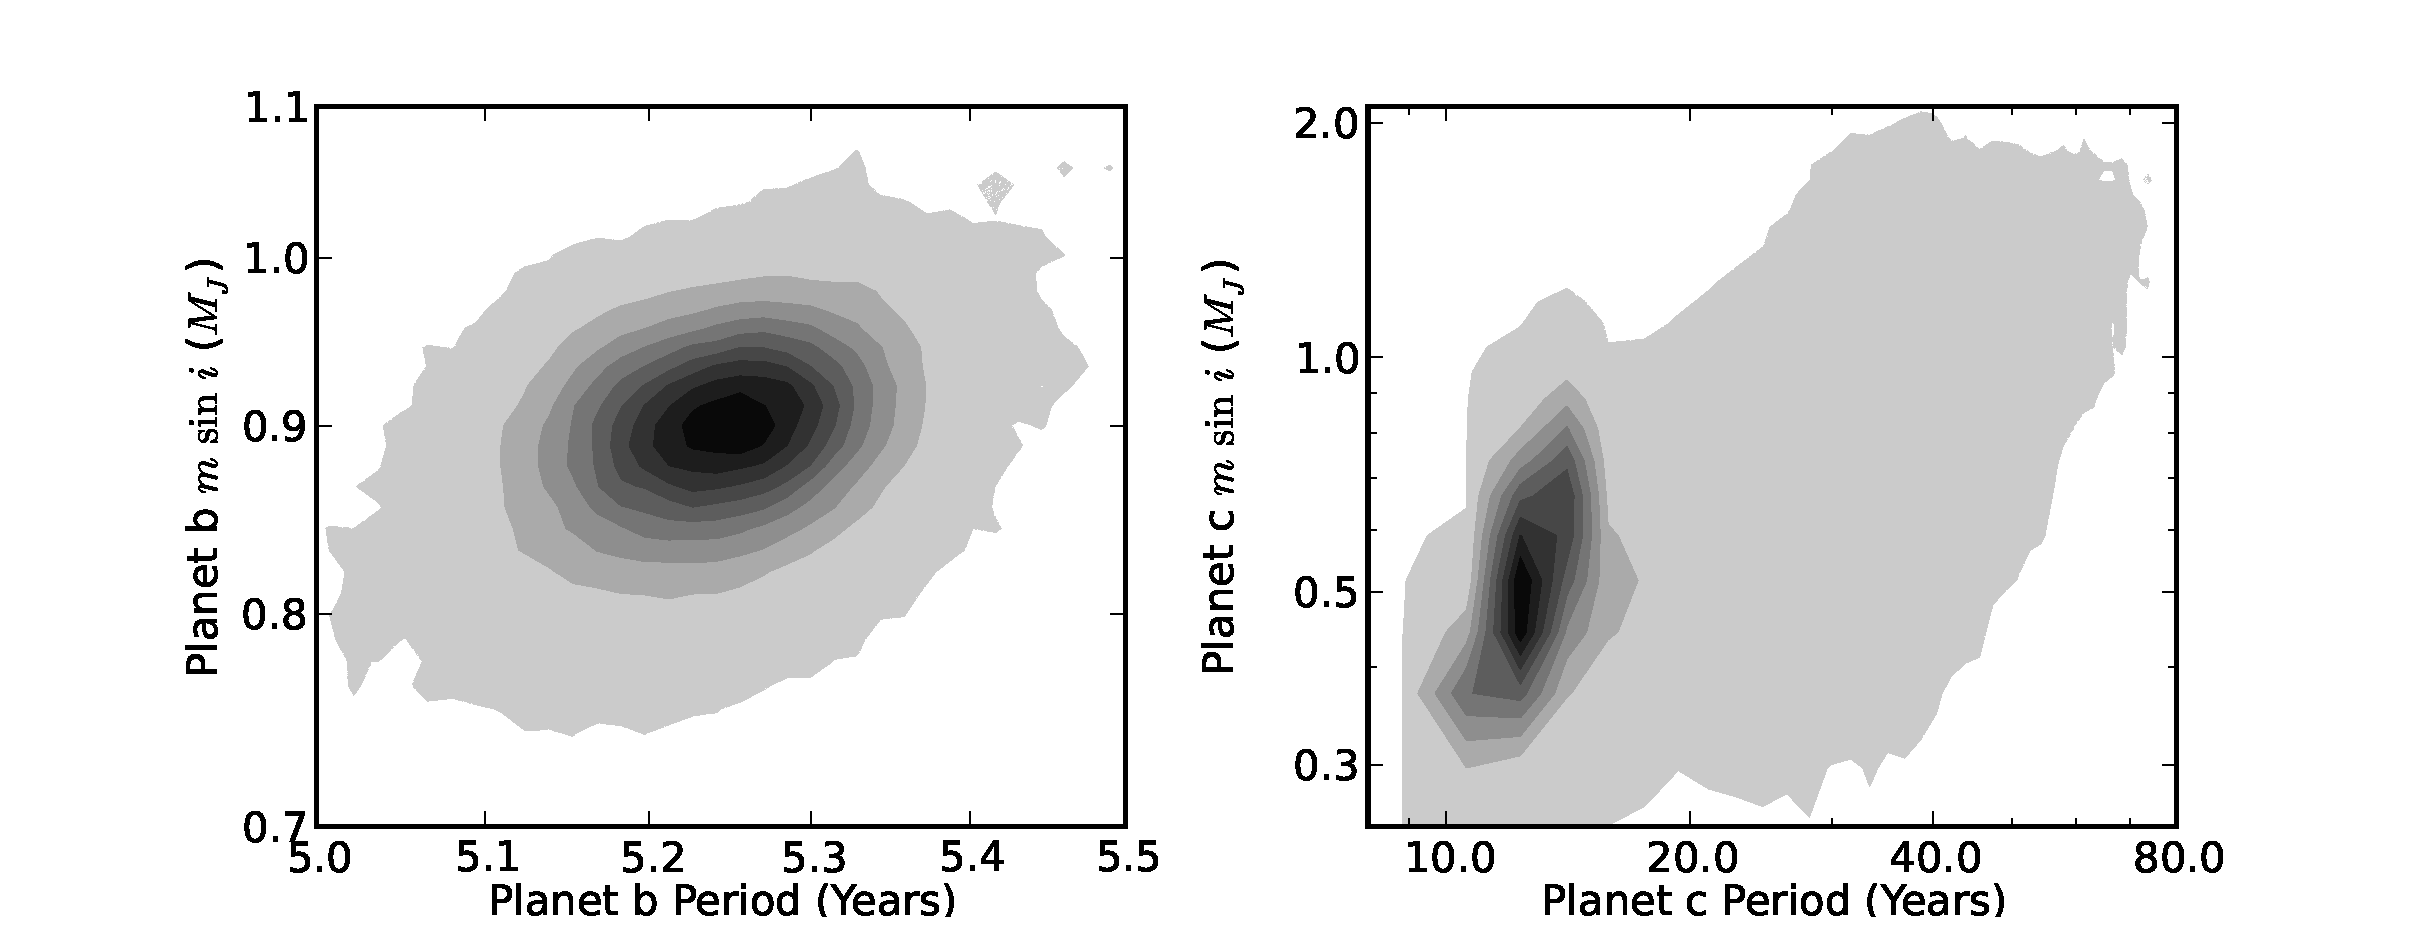
\includegraphics[width=1.0\textwidth]{chapter3/f16.eps}}
\caption[Posterior distributions of allowed masses and periods of 
Gl\,849\,b and Gl\,849\,c]{Position of (left) Gl\,849b and (right) Gl\,849c in the mass-period plane. The orbital parameters for the inner planet are much more tightly constrained than the outer planet. Depending on the exact shape of the planet distribution function, the inner planet may have more than a 50\% probability of being more massive than Jupiter when orientation uncertainties are taken into account.
  }
\label{849}
%\end{landscape}
\end{figure}



\subsection{HIP\,109555}
When observing HIP\,109555 we detected a possible faint companion object located tens of arcseconds away. To prove this companion is not associated with the primary but is instead unrelated, we compare the proper motion of both objects by identifying them in the 2MASS catalog \citep{Skrutskie06} and the Palomar Observatory Sky Survey \citep{Abell59}. Comparing the POSS data collected 16 July 1950 to the 2MASS observation, we detect a proper motion for HIP\,109555 of 0.36 arcsec/yr, consistent with previously published results \citep{vanLeeuwen07}. The hypothetical companion motion, however, is only 5 milliarcseconds per year. Additionally, the companion is bluer in colors derived using the 2MASS J, H, and K filters than HIP\,109555. These are both consistent with the companion being a distant background object, and we neglect its presence in our analysis.

\subsection{HIP\,57050}
\label{HIP57050}
We observed HIP\,57050 (=GJ1148) on December 27, 2012 using the $K_s$ filter on NIRC2. Our imaging is only complete at separations smaller than 1 arcsecond, corresponding to a projected separation of 11 AU. This does not enable us to rule out most stellar companions that could cause our observed RV trends, as shown in Figure \ref{Wright57050}.
\begin{figure}[htbp]
\centerline{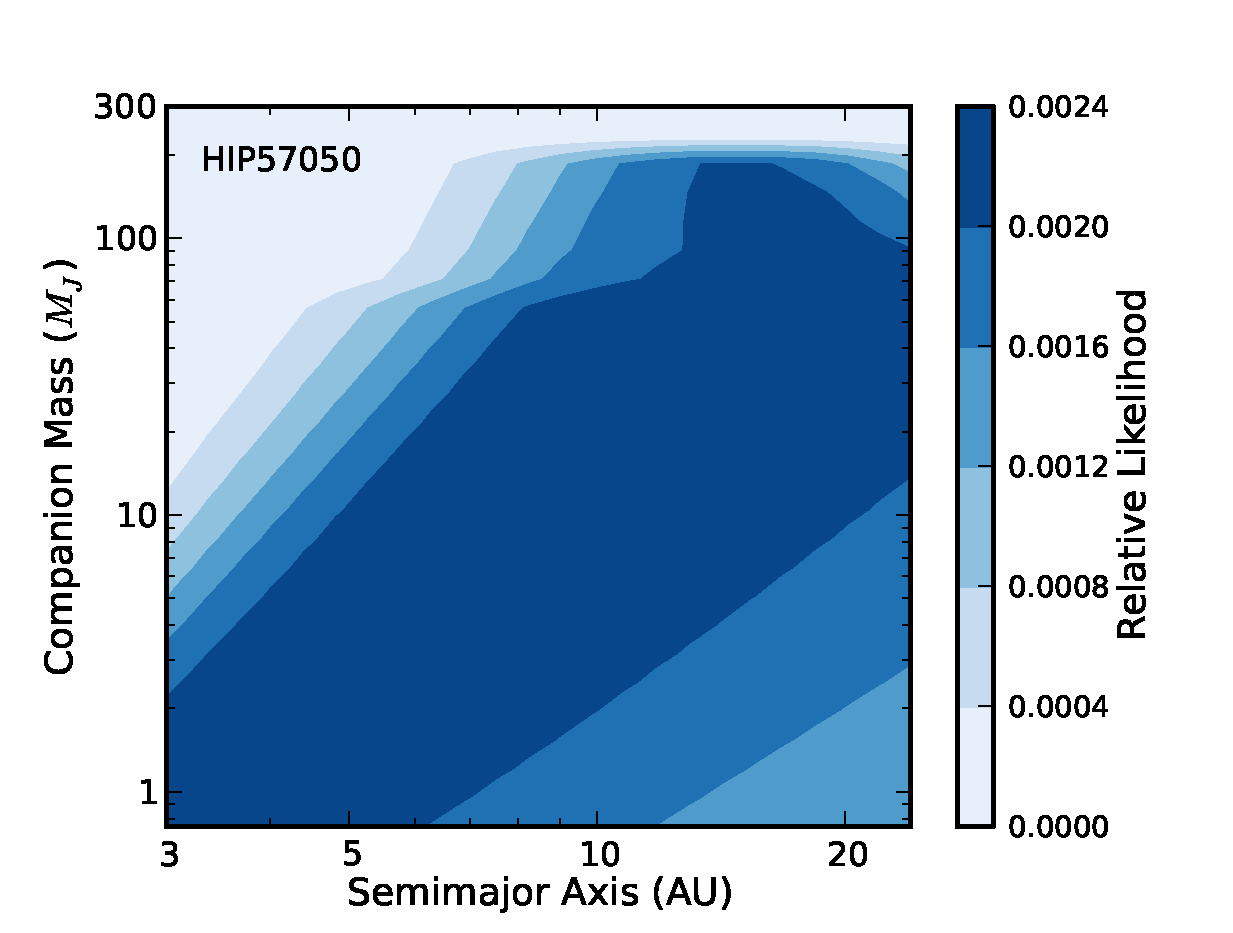
\includegraphics[width=0.75\textwidth]{chapter3/f17.eps}}
\caption[Probability contours displaying the location of a giant companion orbiting HIP\,57050, given that exactly one such planet exists]{Probability contours displaying the location of a giant companion orbiting HIP\,57050, given that exactly one such planet exists, when the RV data is combined with adaptive optics imaging and 2MASS data. Because the AO imagery only extends to 11 AU, there is a small region of parameter space where a low-mass M-dwarf companion could reside. Additional AO observations with a wider field of view would be required to rule out this possibility. Lower-mass companions are allowed in shorter orbital periods due to possible curvature in the radial velocity data.
}
\label{Wright57050}
\end{figure}
If the observed trend is caused by a stellar-mass companion, the companion is likely beyond 10 AU, which corresponds to a separation of 0.9 arcseconds. Thus any stellar companions at their maximum separation that could cause this trend would be expected to be found in a seeing-limited survey. We find no evidence for such a companion. While unlikely, additional AO observations with a wider field of view are required to fully eliminate the possibility that a low-mass star exists. 


\subsection{HIP\,63510}
HIP\,63510B (Ross 458) is an M7 brown dwarf orbiting an M0.5 dwarf at approximately 3 AU \citep{Beuzit04}. Twelve years of RV observations suggest an orbit with a period of 13.9 years, an eccentricity of 0.32, and a minimum mass $m\sin i = 67.9 M_J$, suggesting a nearly edge-on orbit. We estimate a detection efficiency of 1.000 in an RV survey, which is not surprising considering the stellar RV semiamplitude is $K = 1.24$ km s$^{-1}$. This system contains a second companion which is separated from the host star by 1100 AU \citep{Goldman10, Scholz10}

\subsection{HIP\,71898}
HIP\,71898B is an L0 dwarf in a wide orbit around an M3.5 dwarf. \citet{Golimowski04} report a projected separation of $30.01 \pm 3.78$ AU. This target has an RV baseline of 14 years, over which 30 observations were collected. From these observations we measure an acceleration of $8.6 \pm 0.4$ m s$^{-1}$ yr$^{-1}$. At 30 AU, this would suggest a minimum dynamical mass $m \sin i > 45 M_J$, consistent with an L0 dwarf. A detectability plot for companions to HIP\,71898 is shown in Figure \ref{71898}. The observed acceleration lies near a contour representing a 0.9 probability of RV detection, so it is not surprising this companion was detected by CPS. 

\begin{figure}[htbp]
\centerline{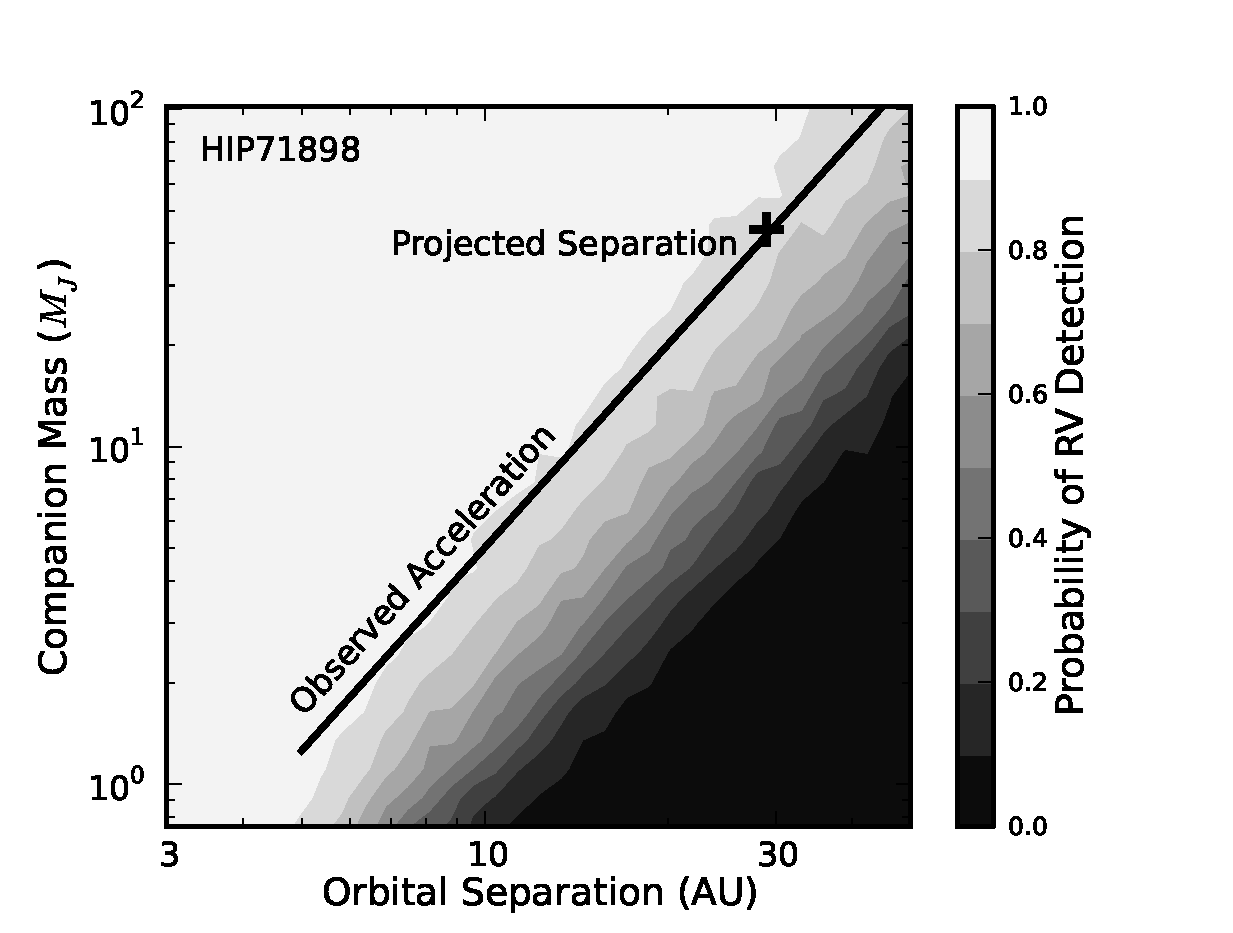
\includegraphics[width=0.75\textwidth]{chapter3/f18.eps}}
\caption[Probability contours displaying the likelihood that a planet of a given mass and semimajor axis would be detected around HIP\,71898 in the CPS RV survey]{ Probability contours displaying the likelihood that a planet of a given mass and semimajor axis would be detected around HIP\,71898 in the CPS RV survey. The diagonal line represents companions that would produce an acceleration of $8.6 \pm 0.4$ m s$^{-1}$ yr$^{-1}$ in an edge on system when the companion was moving along the observer's line of sight. The $+$ marks the spot at which a $45 M_J$ companion at 30 AU would reside; this is the minimum mass and semimajor axis expected from this companion. 
  }
\label{71898}
\end{figure}

\subsection{Gl569}
Gl\,569B is a brown dwarf binary, with an M8.5+M9 pair orbiting each other every $870 \pm 9$ days. The system has a combined mass of $0.140^{+0.009}_{-0.008} M_\odot$ \citep{Dupuy10} and is separated from the primary, an M3.5 dwarf, by a projected separation of 5 arcsec, or 47 AU \citep{Femenia11}. The maximum RV acceleration from such a companion is 3.7 m s$^{-1}$ yr$^{-1}$. For this star, we have a 5.1 year baseline and the median $\sigma$ is 15 m s$^{-1}$. By injecting simulated companions, we estimate an RV detection efficiency near zero for these companions. Thus it is not surprising that it is missed in our sample. 

\subsection{Gl\,229B}
Gl\,229B (HD\,42581) is a T7 dwarf at a projected separation of 44 AU \citep{Faherty09}. This companion has been directly imaged \citep{Nakajima95} but not detected as a strong acceleration through RV variations. As with Gl\,569, this object is beyond our range for efficient brown dwarf detection through RV observations. If we assume a mass of 40 $M_J$, we would expect a maximal RV acceleration of 1.1 m s$^{-1}$ yr$^{-1}$. Thus, again we should not be surprised it is not detected.

\section{A Brief Note on Radial Velocities and Magnetic Activity}
We account for the possibility that any apparent RV accelerations may be induced by magnetic activity statistically, as described in \textsection\ref{FP}. Often, the $S_\textrm{HK}$ value, a measure of the ratio of flux in the Ca II line cores to flux in nearby continuum regions, is taken as a proxy for chromospheric activity \citep{Wilson68, Henry96}. While not a perfect measure, it is comforting to note that the observed radial velocities do not correlate with $S_\textrm{HK}$ in any of our stars with long-term RV accelerations. The RVs for our systems with detected accelerations as well as $S_\textrm{HK}$ for observations after the HIRES detector upgrade are included in Figure \ref{Trendplot} and Table \ref{Txx}. 

\begin{figure}[htbp]
%\begin{landscape}
\centerline{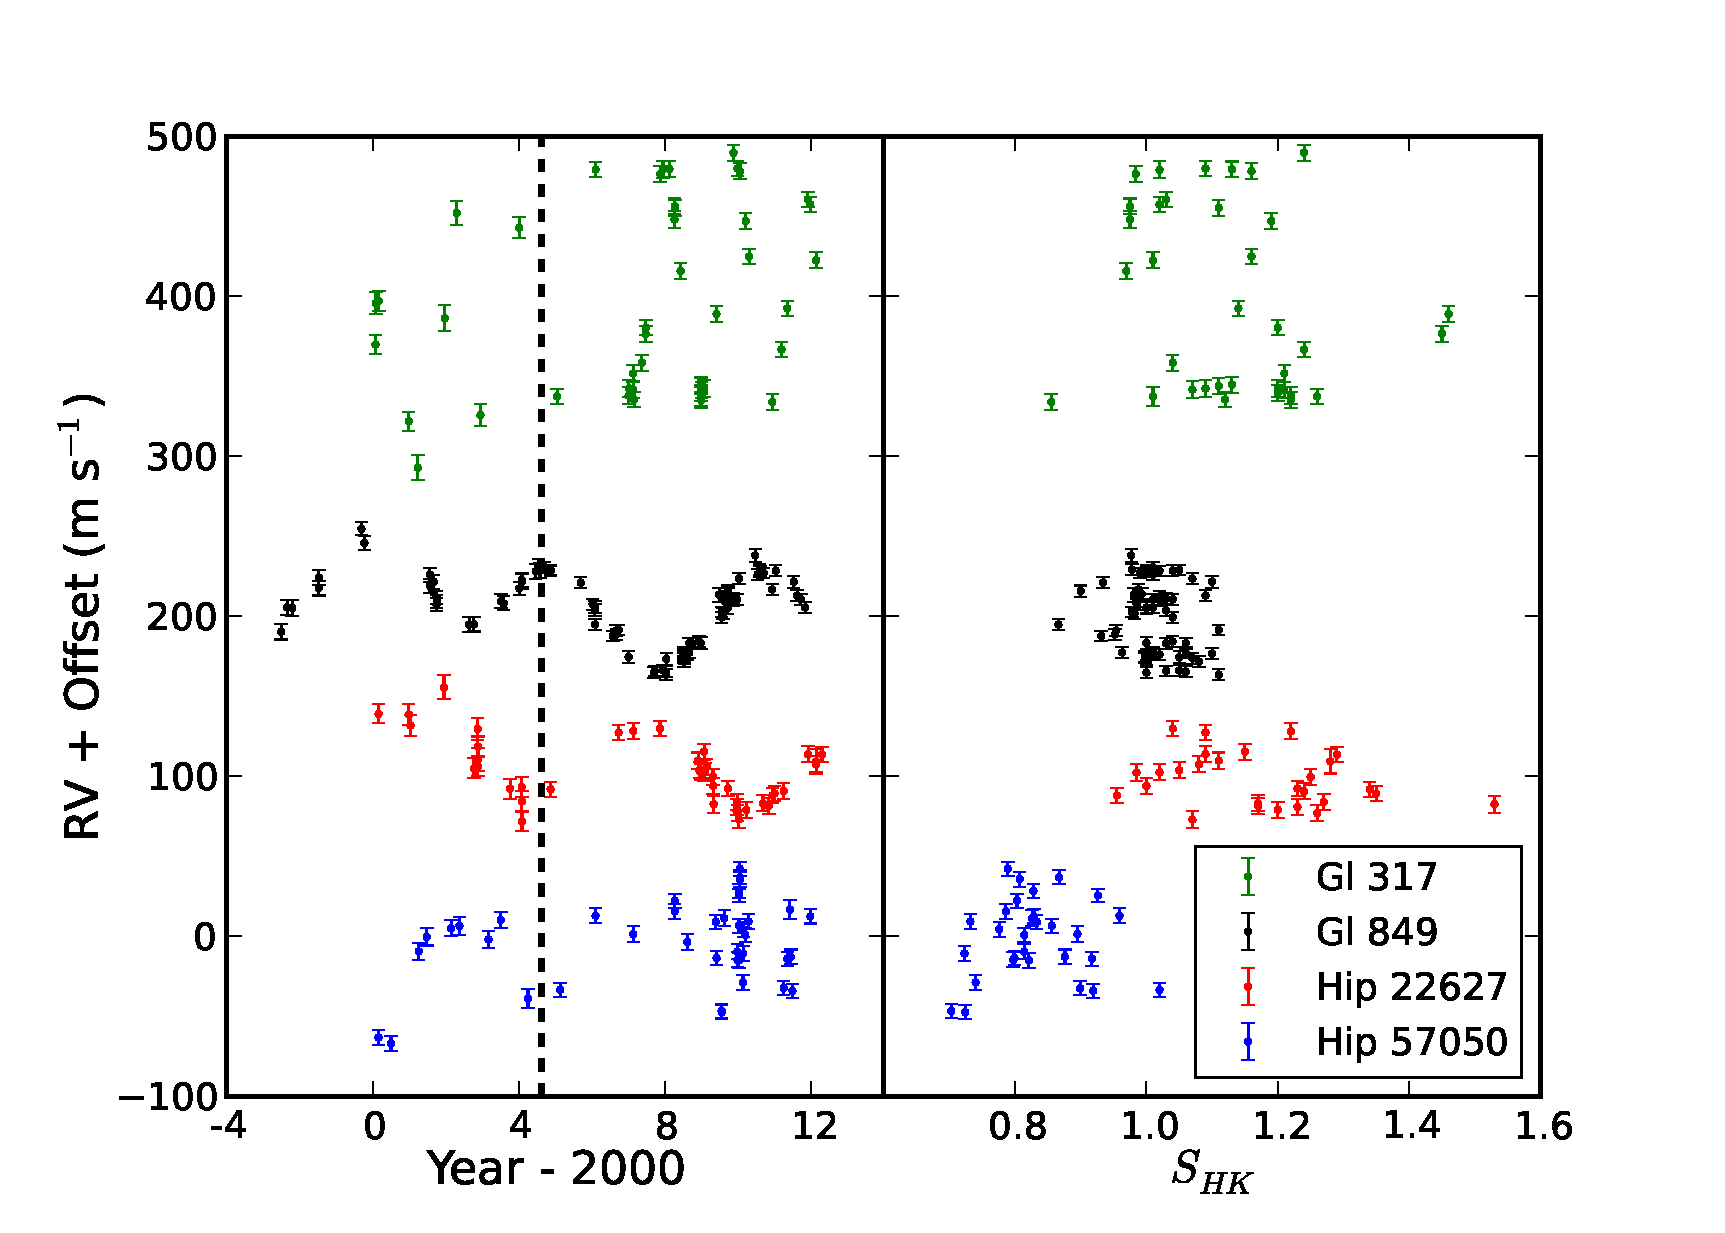
\includegraphics[width=1.0\textwidth]{chapter3/f19.eps}}
\caption[RV time series for our four systems exhibiting long-term RV accelerations and RVs as a function of $S_\textrm{HK}$]{(left) RV time series for our four systems exhibiting long-term RV accelerations. The vertical line in 2004 represents the HIRES detector upgrade in August of that year. (right) RVs as a function of $S_\textrm{HK}$. All four RV accelerations are visible, but none of the RV data appear to correlate with $S_\textrm{HK}$, commonly used as a proxy for stellar chromospheric activity.
  }
\label{Trendplot}
%\end{landscape}
\end{figure}

{\scriptsize
\begin{longtable}{l|ccc||l|ccc} 
\hline
JD-2440000 & RV (m s$^{-1}$) & $\sigma_{\textrm{RV}}$ (m s$^{-1}$) & $S_{\textrm{HK}}$ & JD-2440000 & RV (m s$^{-1}$) & $\sigma_{\textrm{RV}}$ (m s$^{-1}$ & $S_{\textrm{HK}}$ \\
\hline
Gl 317 & & & & & & & \\ 
11550.993 & 369.80 & 5.83 & N/A & 14544.905 & 456.22 & 4.92 & 0.97 \\  
11552.990 & 395.68 & 6.74 & N/A & 14545.894 & 455.37 & 4.96 & 1.11 \\  
11582.891 & 397.16 & 6.08 & N/A & 14603.777 & 415.82 & 5.00 & 0.97 \\  
11883.101 & 321.88 & 5.83 & N/A & 14806.029 & 344.83 & 5.02 & 1.13 \\  
11973.795 & 292.84 & 7.74 & N/A & 14807.069 & 337.39 & 5.70 & 1.01 \\  
12243.073 & 386.34 & 7.95 & N/A & 14808.138 & 343.93 & 4.94 & 1.11 \\  
12362.949 & 451.96 & 7.50 & N/A & 14809.059 & 335.15 & 4.95 & 1.22 \\  
12601.045 & 325.69 & 6.93 & N/A & 14810.161 & 339.65 & 4.87 & 1.20 \\  
12989.125 & 442.81 & 6.64 & N/A & 14811.128 & 341.51 & 4.93 & 1.21 \\  
13369.016 & 337.48 & 4.90 & 1.26 & 14839.107 & 342.36 & 5.26 & 1.09 \\  
13753.983 & 479.22 & 4.85 & 1.13 & 14963.795 & 388.95 & 4.98 & 1.46 \\  
14084.001 & 337.88 & 5.29 & 1.22 & 15134.090 & 489.75 & 4.90 & 1.24 \\  
14086.141 & 342.52 & 5.21 & 1.20 & 15173.079 & 479.92 & 4.79 & 1.09 \\  
14130.082 & 351.80 & 5.37 & 1.21 & 15199.017 & 478.18 & 4.98 & 1.16 \\  
14131.014 & 341.73 & 5.11 & 1.07 & 15255.869 & 447.15 & 4.89 & 1.19 \\  
14138.932 & 335.57 & 4.86 & 1.12 & 15289.857 & 424.86 & 4.82 & 1.16 \\  
14216.733 & 358.57 & 4.95 & 1.04 & 15522.057 & 333.93 & 4.97 & 0.85 \\  
14255.743 & 376.54 & 4.92 & 1.45 & 15613.960 & 366.70 & 4.92 & 1.24 \\  
14255.749 & 380.38 & 4.79 & 1.20 & 15672.848 & 392.45 & 4.92 & 1.14 \\  
14400.110 & 476.46 & 4.91 & 0.98 & 15878.127 & 460.49 & 4.81 & 1.03 \\  
14428.062 & 479.05 & 5.29 & 1.02 & 15903.017 & 457.41 & 4.79 & 1.02 \\  
14492.901 & 479.46 & 5.05 & 1.13 & 15960.986 & 422.57 & 4.98 & 1.01 \\  
14543.948 & 448.01 & 5.34 & 0.97 &  &  &  &  \\  
\hline
Gl 849 & & & & & & & \\ 
10606.068 & 190.31 & 4.78 & N/A & 14455.744 & 165.29 & 3.45 & 1.06 \\  
10666.001 & 205.60 & 4.69 & N/A & 14456.733 & 163.51 & 3.48 & 1.11 \\  
10715.957 & 205.19 & 4.99 & N/A & 14460.742 & 173.41 & 3.53 & 1.00 \\  
10983.038 & 217.69 & 4.67 & N/A & 14634.083 & 176.64 & 3.34 & 1.10 \\  
10984.084 & 224.23 & 4.55 & N/A & 14635.042 & 173.89 & 3.32 & 1.00 \\  
11410.021 & 254.67 & 4.08 & N/A & 14636.051 & 176.71 & 3.33 & 1.01 \\  
11439.865 & 245.85 & 4.30 & N/A & 14637.116 & 176.23 & 3.31 & 1.00 \\  
12095.081 & 225.97 & 4.52 & N/A & 14638.059 & 177.42 & 3.41 & 0.96 \\  
12096.046 & 219.06 & 4.38 & N/A & 14639.067 & 174.78 & 3.42 & 1.00 \\  
12133.013 & 221.49 & 4.39 & N/A & 14640.115 & 171.70 & 3.36 & 1.08 \\  
12160.909 & 211.60 & 4.10 & N/A & 14641.117 & 173.84 & 3.38 & 1.07 \\  
12161.846 & 207.39 & 4.19 & N/A & 14644.113 & 177.39 & 3.40 & 1.01 \\  
12162.887 & 209.34 & 4.22 & N/A & 14674.936 & 176.17 & 3.40 & 1.02 \\  
12486.968 & 194.80 & 4.66 & N/A & 14688.952 & 177.11 & 3.40 & 1.06 \\  
12535.852 & 194.96 & 4.43 & N/A & 14690.005 & 183.22 & 3.51 & 1.06 \\  
12807.011 & 209.44 & 4.30 & N/A & 14721.949 & 183.11 & 3.52 & 1.03 \\  
12834.013 & 208.07 & 4.39 & N/A & 14790.752 & 184.27 & 3.43 & 1.04 \\  
12989.720 & 217.41 & 4.08 & N/A & 14807.793 & 183.33 & 3.47 & 1.00 \\  
13014.710 & 222.75 & 4.27 & N/A & 14989.063 & 213.37 & 4.17 & 0.98 \\  
13015.711 & 221.97 & 4.60 & N/A & 15015.047 & 199.35 & 3.42 & 1.04 \\  
13016.706 & 222.33 & 4.07 & N/A & 15016.074 & 202.71 & 3.36 & 0.98 \\  
13154.080 & 228.16 & 4.76 & N/A & 15029.019 & 201.72 & 3.52 & 0.98 \\  
13180.108 & 231.43 & 4.45 & N/A & 15043.042 & 212.32 & 3.40 & 1.02 \\  
13196.931 & 228.82 & 4.63 & N/A & 15048.996 & 209.45 & 3.39 & 0.98 \\  
13238.929 & 230.55 & 3.44 & 1.01 & 15075.082 & 205.14 & 3.55 & 1.00 \\  
13301.838 & 228.44 & 3.39 & 1.00 & 15080.084 & 215.78 & 3.50 & 0.90 \\  
13302.742 & 228.98 & 3.32 & 1.05 & 15082.073 & 213.97 & 3.44 & 0.99 \\  
13303.798 & 228.40 & 3.27 & 1.02 & 15134.922 & 210.04 & 3.41 & 1.02 \\  
13603.939 & 221.04 & 3.43 & 0.93 & 15135.876 & 210.90 & 3.37 & 1.03 \\  
13724.712 & 207.52 & 3.39 & 0.98 & 15169.797 & 210.64 & 3.55 & 1.01 \\  
13746.715 & 205.70 & 3.60 & 1.01 & 15188.725 & 223.58 & 3.42 & 1.07 \\  
13746.721 & 203.74 & 3.72 & 1.03 & 15352.082 & 238.03 & 4.18 & 0.98 \\  
13749.698 & 194.88 & 3.51 & 0.87 & 15376.032 & 226.26 & 3.36 & 1.01 \\  
13927.015 & 187.71 & 3.42 & 0.93 & 15395.958 & 229.16 & 3.32 & 0.98 \\  
13959.087 & 191.03 & 3.34 & 1.90 & 15397.048 & 227.85 & 3.36 & 1.00 \\  
13960.955 & 188.72 & 3.31 & 0.95 & 15436.111 & 227.10 & 3.40 & 0.99 \\  
13960.962 & 191.05 & 3.32 & 0.95 & 15521.801 & 216.77 & 3.53 & 0.99 \\  
13983.000 & 191.46 & 3.36 & 1.11 & 15555.792 & 228.55 & 3.38 & 1.04 \\  
14083.750 & 174.45 & 3.67 & 1.05 & 15736.122 & 221.64 & 3.86 & 1.10 \\  
14337.074 & 164.82 & 3.45 & 1.00 & 15770.878 & 212.94 & 3.41 & 1.09 \\  
14343.872 & 165.90 & 3.35 & 1.03 & 15807.063 & 210.62 & 3.40 & 1.04 \\  
14429.742 & 166.12 & 3.44 & 1.05 & 15851.759 & 205.57 & 3.33 & 1.00 \\  
\hline
Hip 22627 & & & & & & & \\ 
11580.831 & 139.11 & 6.00 & N/A & 14838.995 & 115.36 & 5.10 & 1.15 \\  
11882.888 & 138.64 & 6.58 & N/A & 14846.957 & 102.80 & 5.28 & 2.81 \\  
11901.002 & 131.80 & 6.77 & N/A & 14864.957 & 105.69 & 5.05 & 1.97 \\  
12235.849 & 155.64 & 7.57 & N/A & 14928.732 & 99.68 & 4.86 & 1.25 \\  
12536.088 & 105.11 & 6.31 & N/A & 14929.726 & 94.02 & 5.14 & 1.00 \\  
12572.991 & 129.52 & 6.78 & N/A & 14934.731 & 82.53 & 5.28 & 1.53 \\  
12573.950 & 118.58 & 6.32 & N/A & 15077.110 & 92.45 & 4.91 & 1.23 \\  
12575.047 & 106.25 & 6.29 & N/A & 15170.784 & 80.88 & 5.08 & 1.23 \\  
12575.991 & 110.57 & 7.00 & N/A & 15170.791 & 84.01 & 5.07 & 1.27 \\  
12898.116 & 92.25 & 6.13 & N/A & 15174.093 & 77.01 & 5.12 & 1.26 \\  
13014.818 & 93.28 & 6.34 & N/A & 15187.837 & 72.99 & 5.07 & 1.07 \\  
13015.832 & 84.39 & 6.15 & N/A & 15261.771 & 79.05 & 5.15 & 1.20 \\  
13016.832 & 71.79 & 5.78 & N/A & 15429.120 & 83.25 & 5.07 & 1.17 \\  
13302.975 & 91.91 & 4.79 & 1.34 & 15487.096 & 81.47 & 4.81 & 1.17 \\  
13984.089 & 127.34 & 4.92 & 1.09 & 15522.938 & 88.05 & 4.89 & 0.95 \\  
14130.853 & 128.24 & 5.10 & 1.22 & 15545.819 & 89.25 & 4.89 & 1.35 \\  
14397.938 & 129.88 & 4.87 & 1.04 & 15636.775 & 90.74 & 4.87 & 1.24 \\  
14778.991 & 109.83 & 5.06 & 1.11 & 15879.984 & 113.81 & 4.90 & 1.09 \\  
14790.995 & 103.81 & 5.07 & 1.05 & 15960.761 & 109.29 & 7.51 & 1.28 \\  
14807.917 & 102.51 & 4.97 & 1.02 & 15960.765 & 107.53 & 4.93 & 1.08 \\  
14838.988 & 102.33 & 5.11 & 0.98 & 16019.733 & 113.58 & 4.78 & 1.29 \\  
\hline
Hip 57050 & & & & & & & \\ 
11581.046 & -63.25 & 4.53 & N/A & 15172.138 & -9.58 & 4.64 & 0.81 \\  
11705.827 & -67.09 & 4.79 & N/A & 15174.138 & -14.72 & 4.67 & 0.80 \\  
11983.009 & -9.42 & 5.27 & N/A & 15188.151 & -14.99 & 4.64 & 0.82 \\  
12064.864 & -0.39 & 5.34 & N/A & 15189.155 & 6.60 & 4.25 & 0.86 \\  
12308.077 & 4.98 & 5.01 & N/A & 15190.153 & 25.56 & 4.11 & 0.93 \\  
12391.034 & 6.53 & 5.63 & N/A & 15191.133 & 28.40 & 4.36 & 0.83 \\  
12681.050 & -1.92 & 5.15 & N/A & 15197.136 & 42.23 & 4.28 & 0.79 \\  
12804.885 & 10.26 & 5.05 & N/A & 15198.054 & 35.70 & 4.59 & 0.81 \\  
13077.104 & -38.83 & 5.83 & N/A & 15199.170 & 36.95 & 4.42 & 0.87 \\  
13398.975 & -33.44 & 4.33 & 1.02 & 15229.114 & -28.84 & 4.45 & 0.74 \\  
13753.068 & 12.88 & 4.64 & 0.96 & 15229.958 & -10.72 & 4.71 & 0.72 \\  
14131.092 & 1.32 & 4.96 & 0.90 & 15232.054 & 4.35 & 4.63 & 0.78 \\  
14545.002 & 15.61 & 4.55 & 0.79 & 15251.997 & 0.76 & 4.38 & 0.81 \\  
14546.007 & 22.29 & 4.29 & 0.80 & 15284.858 & 9.29 & 4.64 & 0.73 \\  
14671.811 & -3.54 & 5.13 & 5.32 & 15636.023 & -32.36 & 4.31 & 0.90 \\  
14955.894 & 9.12 & 4.47 & 0.83 & 15671.915 & -13.93 & 4.34 & 0.92 \\  
14963.930 & -13.66 & 4.43 & 0.80 & 15698.820 & 16.56 & 5.97 & 7.95 \\  
15014.782 & -46.65 & 4.50 & 0.70 & 15707.812 & -12.89 & 4.66 & 0.88 \\  
15015.804 & -47.40 & 4.41 & 0.72 & 15723.769 & -34.04 & 4.41 & 0.92 \\  
15041.758 & 11.31 & 5.04 & 0.83 & 15903.064 & 12.42 & 4.40 & 0.83  \\
\hline
\caption{RVs and $S_{\textrm{HK}}$ values for systems with long-term RV accelerations}
\label{Txx}
\end{longtable}
}






\chapter{This is the Fourth Chapter}
\label{chap:lhs1}

\btmtodo{This is LHS Part 1}
\chapter{This is the Fifth Chapter}

\btmtodo{This is LHS Part II}
\label{chap:lhsspitz}

\chapter{This is the Sixth Chapter}
\label{chap:Mbinaries}

\btmtodo{This is the M+M binary work}

\chapter{This is the Seventh Chapter}
\label{chap:k2}

\btmtodo{This is the K2 planet catalog}

\chapter{This is the Eighth Chapter}
\label{chap:wfirst}

\begin{figure}[hbt!]
\centering

\includegraphics[width=.3\textwidth]{caltech.png}
\caption[Example Figure]{This is a figure}
\label{fig:logo}
\end{figure}

\subsection{This is a subsection}

\begin{table}[hbt!]
\centering
\begin{tabular}{ll}
\hline
Area & Count\\
\hline
North & 100\\
South & 200\\
East & 80\\
West & 140\\
\hline
\end{tabular}
\caption[Table]{This is a table}
\label{tab:sample}
\end{table}

\btmtodo{This is WFIRST}
\btmtodo{Replace arXiv listings in bibliography that are old}

\chapter{Summary and Future Directions}
\label{chap:summary}

This thesis has focused on the study of low-mass stars and their companions,
whether these companions are planets, brown dwarfs, or themselves other M dwarfs.
While this work has been able to advance the study of all three of these classes of
objects, there is more that can be done in the future as new data are collected and new
instruments are built at new facilities.
Let us consider each of these classes of objects in turn.

In Chapter \ref{chap:trends}, I developed a method to measure the occurrence rate of giant
planets out to 20 AU through a combination of high-contrast direct imaging and 
detections of long-term RV trends.
The planets inferred in this work form a unique region of parameter space as yet 
inaccessible to searches via other methods:
they are too far from their host stars to be detectable through transit searches,
but too near and too faint to be detectable through direct imaging campaigns alone.
The method developed here is directly applicable to higher-mass host stars, and the
process can be extended to directly measure the occurrence rate of planets around K and G
stars.
With the larger number of G and K dwarfs observed in RV surveys and the longer observational
time baseline, it is possible that we will be able to measure the occurrence rate of 
giant planets around these stars to an even higher precision.
Some of this work is ongoing, while the \textit{Gaia} telescope will provide more  information about Jupiter-like planets in the Solar neighborhood in the second half of
this decade.
In Chapter \ref{chap:k2} I presented a method to understand the stellar and planetary parameters of candidate systems uncovered by \KT, a process that can also be applied to the systems detected by \textit{WFIRST} (Chapter \ref{chap:wfirst}. 
\KT\ will enable us to better understand the population of planets orbiting M dwarfs 
in the Solar neighborhood. 
By the end of the mission, \KT\ will search for transit signals
around as many as 50,000 M dwarfs, while the original \kep\ mission observed 5,000.
Moreover, \KT\ will observe mid-M dwarfs, where the original \kep\ mission largely eschewed
stars later than M1.
Both \KT\ and \textit{WFIRST} will target higher mass stars in vastly different galactic
environments: \KT\ has targeted young clusters, stars in and well out of the galactic 
plane, and stars at varied galactocentric distances.
\textit{WFIRST} will similarly be able to detect transits around solar-type stars
more than 2 kiloparsec away in the direction of the galactic bulge. 
Following the galactic metallicity gradient of \citep{Rolleston00}, in which the 
metallicity of stars decreases at $0.07 \pm 0.01$ dex kpc$^{-1}$, we might expect
these stars to host Jupiter-sized planets 50\% more frequently than stars
near the Sun.
\textit{WFIRST} will enable us to test theories of planet formation and the relation
between stellar metallicity and planet formation with unprecendented detail.

Next, we turn our attention to brown dwarfs.
In Chapters \ref{chap:lhs1} and \ref{chap:lhsspitz} I presented LHS\,6343\,C, the
brown dwarf with the most precise radius measurement and the only brown dwarf with a
direct mass, radius, and luminosity measurement.
LHS\,6343\,C can provide a single test of brown dwarf models, but more similar
brown dwarfs are required.
Fortunately, more similar brown dwarfs are being discovered. 
In 2016, \citet{Bayliss16} presented radial velocity data on EPIC\,201702477\,b,
one of the objects of interest characterized in Chapter \ref{chap:k2}. 
I was not able to confirm or rule out the planetary nature of this system;
with radial velocities, these authors were able to confirm the system as a transiting
brown dwarf with a period of 40.74 days.
Similarly, other work has discovered a transiting brown dwarf in the 3 Gyr Ruprecht 147
cluster (Curtis et al.\ \textit{in prep}). 
As more systems like these are discovered, especially systems with known ages, 
we will be able to fill the brown dwarf mass-radius diagram and connect the transiting
brown dwarf population to the field brown dwarf population, for which direct measurements
of masses and radii are impossible.


Finally, we consider M+M binaries. 
Throughout the M dwarf spectral class, more objects with direct mass measurements are
needed.
Nearly all mass measurements come from eclipsing binaries in short periods, which may
cause inflated radii due to magnetic activity \citep{Chabrier07, Jackson09}.
\KT\ and \textit{WFIRST} will enable the discovery of more M dwarf eclipsing binaries 
on longer periods, which are less likely to be inflated.
In Chapter \ref{chap:ttvs}, I describe a method to measure masses of single stars
with transiting planets by combining RV and TTV observations of the planetary system,
avoiding the potential complications of binary stars entirely.

Very young stars rotate rapidly and are photometrically very active, complicating both
the detection of transiting planets and the precision RVs required to confirm them 
directly.
The problems with stellar models at these ages are even worse, with only a handful of
M dwarfs younger than 100 Myr having directly measured masses.
In Chapter \ref{chap:Mbinaries} I presented GJ\,3305\,AB, a binary M+M system in the
$\beta$ Pictoris young moving group. 
I measured the mass of both components, comparing them to stellar models.
This is only one binary system of the dozens I am monitoring astrometrically and through
RV observations with collaborators. There are more than 20 more stars in more than 
10 systems with orbits that have closed or will close in the next few years in the same
mass and age range.
As these orbits close, we will develop a population of stars with measured masses to
compare against models, enabling the development of the next generation of stellar models.

Of course, much of the future work will rely on future instruments and future telescopes
both in the ground and in space. 
In this thesis I discuss the ongoing \KT\ and future \textit{WFIRST} missions.
beyond these, the study of M dwarfs can look forward to contributions from future 
transit search missions like \textit{TESS} \citep{Ricker14} and \textit{PLATO} \citep{Catala10}, as well as the 
development and construction of the next generation of 30-meter class telescopes.
Moreover, RV instruments that are optimized for observations in the near-IR, such as
\textit{iLocator} \citep{Crepp14} and \textit{MAROON-X} \citep{Seifahrt16}, will enable
later, more distant M dwarfs to be more easily targeted in RV surveys.
While the equations of stellar structure force M dwarfs to be faint, their future
is very bright indeed.



\printbibliography[]
%\bibliography{exopapers}

%\appendix

%\chapter{Questionnaire}
%\chapter{Consent Form}

%\printindex

%\theendnotes

%% Pocket materials at the VERY END of thesis
%\pocketmaterial
%\extrachapter{Pocket Material: Map of Case Study Solar Systems} 


\end{document}
